\documentclass{memoir}
\usepackage[dvipsnames]{xcolor} % Required for specifying custom colors
\usepackage[showframe=false]{geometry} % Required for adjusting page dimensions and margins
\usepackage[colorlinks=true, linkcolor=blue, citecolor=blue, urlcolor=blue]{hyperref}
% Packages for custom shapes and boxes
\usepackage{tikz} % Required for drawing custom shapes
\usepackage[framemethod=TikZ]{mdframed} % Required for creating the theorem, definition, exercise and corollary boxes
% \newcounter{theo}[section]\setcounter{theo}{0}

% THEOREM BOXES
\newcounter{theo}[section]\setcounter{theo}{0}
\renewcommand{\thetheo}{\arabic{section}.\arabic{theo}}

\newenvironment{theo}[2][]{%
    \refstepcounter{theo}

    \ifstrempty{#1}%
    % if condition (without title)
    {\mdfsetup{%
            frametitle={%
                    \tikz[baseline=(current bounding box.east),outer sep=0pt]
                    \node[anchor=east,rectangle,fill=black,text=white]
                    {\strut Theorem~\thetheo};}
        }%
        % else condition (with title)
    }{\mdfsetup{%
            frametitle={%
                    \tikz[baseline=(current bounding box.east),outer sep=0pt]
                    \node[anchor=east,rectangle,fill=black,text=white]
                    {\strut Theorem~\thetheo:~#1};}%
        }%
    }%
    % Both conditions
    \mdfsetup{%
        innertopmargin=6pt,innerbottommargin=12pt,linecolor=black,%
        linewidth=2pt,topline=true,%
        frametitleaboveskip=\dimexpr-\ht\strutbox\relax%
    }

    \begin{mdframed}[]\relax}{
    \end{mdframed}}

% DEFINITION BOXES
\newcounter{Def}[section]\setcounter{Def}{0}
\renewcommand{\theDef}{\arabic{section}.\arabic{Def}}

\newenvironment{Def}[2][]{%
    \refstepcounter{Def}

    \ifstrempty{#1}%
    % if condition (without title)
    {\mdfsetup{%
            frametitle={%
                    \tikz[baseline=(current bounding box.east),outer sep=0pt]
                    \node[anchor=east,rectangle,fill=black,text=white]
                    {\strut Definition~\theDef};}
        }%
        % else condition (with title)
    }{\mdfsetup{%
            frametitle={%
                    \tikz[baseline=(current bounding box.east),outer sep=0pt]
                    \node[anchor=east,rectangle,fill=black,text=white]
                    {\strut Definition~\theDef:~#1};}%
        }%
    }%
    % Both conditions
    \mdfsetup{%
        innertopmargin=6pt,
        innerbottommargin=12pt,
        linecolor=black,%
        linewidth=2pt,topline=true,%
        frametitleaboveskip=\dimexpr-\ht\strutbox\relax%
    }

    \begin{mdframed}[]\relax}{%
    \end{mdframed}}


% TIP BOXES
\newcounter{Tip}[section]\setcounter{Tip}{0}
\renewcommand{\theTip}{\arabic{section}.\arabic{Tip}}

\newenvironment{Tip}{%
    \refstepcounter{Tip}
    \mdfsetup{%
        backgroundcolor=OliveGreen!10,
        innertopmargin=12pt,
        innerbottommargin=12pt,
        linecolor=black,
        linewidth=0pt,
        topline=false,
        frametitleaboveskip=\dimexpr-\ht\strutbox\relax
    }
    \begin{mdframed}[]\relax
        \textbf{Tip:}
        }{%
    \end{mdframed}
}

% GREEN BOXES
\newenvironment{greenbox}{%
    \mdfsetup{%
        backgroundcolor=OliveGreen!10,
        innertopmargin=12pt,
        innerbottommargin=12pt,
        linecolor=black,
        linewidth=0pt,
        topline=false,
        frametitleaboveskip=\dimexpr-\ht\strutbox\relax
    }
    \begin{mdframed}[]\relax

        }{%
    \end{mdframed}
}

% GRAY BOXES
\newenvironment{graybox}{%
    \mdfsetup{%
        backgroundcolor=black!10,
        innertopmargin=12pt,
        innerbottommargin=12pt,
        linecolor=black,
        linewidth=0pt,
        topline=false,
        frametitleaboveskip=\dimexpr-\ht\strutbox\relax
    }
    \begin{mdframed}[]\relax

        }{%
    \end{mdframed}
}

% NOTE BOXES
\newcounter{Note}[section]\setcounter{Note}{0}
\renewcommand{\theNote}{\arabic{section}.\arabic{Note}}

\newenvironment{Note}{%
    \refstepcounter{Note}
    \mdfsetup{%
        backgroundcolor=black!10,
        innertopmargin=10pt,
        innerbottommargin=8pt,
        linecolor=black,
        linewidth=0pt,
        topline=false,
        frametitleaboveskip=\dimexpr-\ht\strutbox\relax
    }
    \begin{mdframed}[]\relax
        }{%
    \end{mdframed}
}

% GENERIC BOXES

\newenvironment{gbox}{%
    \mdfsetup{%
        backgroundcolor=white,
        innertopmargin=12pt,
        innerbottommargin=6pt,
        linecolor=black,
        linewidth=1pt,
        topline=true,
        frametitleaboveskip=\dimexpr-\ht\strutbox\relax
    }
    \begin{mdframed}[]\relax
        % Your content goes here
        }{%
    \end{mdframed}
}

% PROOF BOXES

% \newcounter{theo}[section]\setcounter{theo}{0}

% PROOF BOXES

\newcounter{Proof}[section]\setcounter{Proof}{0}
\renewcommand{\theProof}{\arabic{section}.\arabic{Proof}}

\newenvironment{Proof}[1][]{%
    \refstepcounter{Proof}

    \ifstrempty{#1}%
    % if condition (without title)
    {\mdfsetup{%
            frametitle={%
                    \tikz[baseline=(current bounding box.east),outer sep=0pt]
                    \node[anchor=east,rectangle,fill=white,text=black]
                    {\strut Proof~\theProof};}
        }%
        % else condition (with title)
    }{\mdfsetup{%
            frametitle={%
                    \tikz[baseline=(current bounding box.east),outer sep=0pt]
                    \node[anchor=east,rectangle,fill=white,text=black]
                    {\strut Proof~\theProof:~#1};}%
        }%
    }%
    % Both conditions
    \mdfsetup{%
        innertopmargin=6pt,
        innerbottommargin=12pt,
        linecolor=black,%
        linewidth=1pt,topline=true,%
        frametitleaboveskip=\dimexpr-\ht\strutbox\relax%
    }

    \begin{mdframed}[]\relax}{
        \hfill$\blacksquare$
    \end{mdframed}
}

% EXAMPLE BOXES

\newcounter{Example}[section]\setcounter{Example}{0}
\renewcommand{\theExample}{\arabic{section}.\arabic{Example}}

\newenvironment{Example}[1][]{%
    \refstepcounter{Example}

    \ifstrempty{#1}%
    % if condition (without title)
    {\mdfsetup{%
            frametitle={%
                    \tikz[baseline=(current bounding box.east),outer sep=0pt]
                    \node[anchor=east,rectangle,fill=white,text=black]
                    {\strut Example~\theExample};}
        }%
        % else condition (with title)
    }{\mdfsetup{%
            frametitle={%
                    \tikz[baseline=(current bounding box.east),outer sep=0pt]
                    \node[anchor=east,rectangle,fill=white,text=black]
                    {\strut Example~\theExample:~#1};}%
        }%
    }%
    % Both conditions
    \mdfsetup{%
        innertopmargin=6pt,
        innerbottommargin=12pt,
        linecolor=black,%
        linewidth=1pt,topline=true,%
        frametitleaboveskip=\dimexpr-\ht\strutbox\relax%
    }

    \begin{mdframed}[]\relax}{
        \hfill$\blacksquare$
    \end{mdframed}
}

% Function Counter
\newcounter{Func}[section]
\renewcommand{\theFunc}{\arabic{section}.\arabic{Func}}

% Function Environment
\newenvironment{Func}[1][]{
    \refstepcounter{Func}
    \ifstrempty{#1}% 
    {% If no title is provided
        \mdfsetup{
            frametitle={
                \tikz[baseline=(current bounding box.east),outer sep=0pt]
                \node[anchor=east,rectangle,fill=black,text=white]
                {\strut Function~\theFunc};}
        }
    }{% If a title is provided
        \mdfsetup{
            frametitle={
                \tikz[baseline=(current bounding box.east),outer sep=0pt]
                \node[anchor=east,rectangle,fill=black,text=white]
                {\strut Function~\theFunc:~#1};}
        }
    }
    % Common settings for both cases
    \mdfsetup{
        innertopmargin=10pt,
        innerbottommargin=10pt,
        skipabove=\baselineskip,
        skipbelow=\baselineskip,
        linecolor=black,
        linewidth=1pt,
        topline=true,
        frametitleaboveskip=\dimexpr-\ht\strutbox\relax,
        frametitlealignment=\raggedright
    }
    \begin{mdframed}
}{
    \end{mdframed}
}

 % This file contains the code for the boxes
\usepackage{listings}

% Define OCaml language style
\lstdefinelanguage{OCaml}{
  morekeywords={let, rec, if, then, else, print_endline, in, match, with, type},
  sensitive=true,
  morecomment=[s]{(*}{*)},
  morestring=[b]",
}

% Define Python language style
\lstdefinelanguage{Python}{
  morekeywords={def, return, if, else, print},
  sensitive=true,
  morecomment=[l]{\#},
  morestring=[b]",
}

% Define Ubuntu Terminal style
\lstdefinelanguage{Bash}{
  morekeywords={ls, cd, mkdir, rm, mv, cp, touch, echo, sudo, pwd, cat, vim, nano, apt, apt-get, chmod, chown, bash},
  sensitive=true,
  morecomment=[l]{\#}, % Single-line comments start with #
  morestring=[b]",      % Strings are enclosed in double quotes
}

% Set up general style for the terminal
\lstset{
  basicstyle=\ttfamily\small\color{white},  % Text in white for visibility on black
  keywordstyle=\color{cyan}\bfseries,      % Commands in cyan
  commentstyle=\color{green},              % Comments in green
  stringstyle=\color{yellow},              % Strings in yellow
  frame=single,
  showstringspaces=false,
  breaklines=true,
  backgroundcolor=\color{black},           % Black background
  numbers=left,                             % Add line numbers on the left
  numberstyle=\tiny\color{gray},           % Line numbers in gray
}

\lstdefinelanguage{PlainText}{
  morekeywords={},
  sensitive=false,
  morecomment=[l]{\#},
  morestring=[b]"
}

% Command for dark background (!20)
\newcommand{\snippet}[1]{\colorbox{OliveGreen!20}{\texttt{#1}}}

\newcommand{\texttr}[1]{\texttt{\color{red}{#1}}}
\newcommand{\texttb}[1]{\texttt{\color{blue}{#1}}} % This file contains the code for the code listings
\usepackage{adjustbox} % Required for fitting tables into the page width


% Packages for math symbols and images
\usepackage{amssymb} % Math symbols such as \mathbb
\usepackage{amsmath} % Required for \begin{align}...\end{align}
\DeclareMathOperator{\lcm}{lcm}
\usepackage{mathtools}
\DeclarePairedDelimiter\ceil{\lceil}{\rceil}
\DeclarePairedDelimiter\floor{\lfloor}{\rfloor}
\usepackage{graphicx} % Required for including images

% Tables
\usepackage{multirow} % Required for creating multirow cells in tables
\usepackage{array} % Required for creating tables
\usepackage{colortbl} % Add this line to import the colortbl package
\setlength{\tabcolsep}{18pt} % Default value: 6pt
\renewcommand{\arraystretch}{1.5} % Default value: 1
\usepackage{changepage} % Required for adjusting the width of the table


% Package for customizing captions
\usepackage{caption}  % Required for customizing captions

\usepackage{setspace} % Required for adjusting line spacing
\usepackage{etoolbox} % For \ifstrempty

\usepackage{subcaption} % for subfigures

\usepackage[linesnumbered, noend]{algorithm2e}
\usepackage{algpseudocode}
\usepackage{makecell} % for line break in table cell

\usepackage{longdivision}% Package for long division algorithm
\usepackage{enumitem}
\usepackage{xlop} % For long addition
% commands

% Tikz
% \tikzset{
%     pics/machine/.style={
%             code={
%                     \coordinate (-in) at ({-0.5*\pgfkeysvalueof{/tikz/machine/width}},0);
%                     \coordinate (-out) at ({0.5*\pgfkeysvalueof{/tikz/machine/width}},0);
%                     \coordinate (-north) at (0,{0.5*\pgfkeysvalueof{/tikz/machine/height}});
%                     \coordinate (-south) at (0,{-0.5*\pgfkeysvalueof{/tikz/machine/height}});
%                     \path[/tikz/machine/filling]
%                     ([shift={(-0.75em,0.5em)}]-in)
%                     -- ([shift={(0,0.25em)}]-in)
%                     -- ([shift={(0,-5pt)}]-north -| -in)
%                     arc[start angle=180, end angle=90, radius=5pt]
%                     -- ([shift={(-5pt,0)}]-north -| -out)
%                     arc[start angle=90, end angle=0, radius=5pt]
%                     -- ([shift={(0,0.25em)}]-out)
%                     -- ([shift={(0.75em,0.5em)}]-out)
%                     -- ([shift={(0.75em,-0.5em)}]-out)
%                     -- ([shift={(0,-0.25em)}]-out)
%                     -- ([shift={(0,5pt)}]-south -| -out)
%                     arc[start angle=360, end angle=270, radius=5pt]
%                     -- ([shift={(5pt,0)}]-south -| -in)
%                     arc[start angle=270, end angle=180, radius=5pt]
%                     -- ([shift={(0,-0.25em)}]-in)
%                     -- ([shift={(-0.75em,-0.5em)}]-in)
%                     -- cycle;
%                     \draw[/tikz/machine/border]
%                     ([shift={(-0.75em,0.5em)}]-in)
%                     -- ([shift={(0,0.25em)}]-in)
%                     -- ([shift={(0,-5pt)}]-north -| -in)
%                     arc[start angle=180, end angle=90, radius=5pt]
%                     -- ([shift={(-5pt,0)}]-north -| -out)
%                     arc[start angle=90, end angle=0, radius=5pt]
%                     -- ([shift={(0,0.25em)}]-out)
%                     -- ([shift={(0.75em,0.5em)}]-out);
%                     \draw[/tikz/machine/border]
%                     ([shift={(0.75em,-0.5em)}]-out)
%                     -- ([shift={(0,-0.25em)}]-out)
%                     -- ([shift={(0,5pt)}]-south -| -out)
%                     arc[start angle=360, end angle=270, radius=5pt]
%                     -- ([shift={(5pt,0)}]-south -| -in)
%                     arc[start angle=270, end angle=180, radius=5pt]
%                     -- ([shift={(0,-0.25em)}]-in)
%                     -- ([shift={(-0.75em,-0.5em)}]-in);
%                     \node (-node) at (0,0) {#1};
%                 }
%         },
%     machine/width/.initial={10.5em},
%     machine/height/.initial={5em},
%     machine/filling/.style={
%             left color=cyan!50!OliveGreen!25,
%             right color=cyan!50!OliveGreen!25,
%             middle color=cyan!50!OliveGreen!10
%         },
%     machine/border/.style={
%             OliveGreen!50!cyan
%         }
% }

% Color Text
\definecolor{BlueText}{RGB}{0,51,204}
\newcommand{\bt}[1]{\textcolor{BlueText}{#1}}

\newcommand{\Div}{%
    \par\noindent\hrulefill\par
}

\renewcommand{\clearforchapter}{ \newpage}

\makeatletter
\NewCommandCopy\@@pmod\pmod
\DeclareRobustCommand{\pmod}{\@ifstar\@pmods\@@pmod}
\def\@pmods#1{\mkern4mu({\operator@font mod}\mkern 6mu#1)}
\makeatother

\definecolor{Wine}{RGB}{128,0,0}

\newcolumntype{g}{>{\columncolor{OliveGreen!10}}c}

\newcommand{\qres}{(\mathbb{Z}_p^*)^2}
\newcommand{\ires}{(\mathbb{Z}_n^*)^2}
\newcommand{\pres}{\mathbb{Z}_p^*}
\newcommand{\peres}{\mathbb{Z}_{p^{e}}^*}
\newcommand{\gres}{\mathbb{Z}_n}
\newcommand{\Z}{\mathbb{Z}}


\algnewcommand\algorithmicforeach{\textbf{for each}}
\algdef{S}[FOR]{ForEach}[1]{\algorithmicforeach\ #1\ \algorithmicdo}

\newcommand*{\carry}[1][1]{\overset{#1}}
\newcolumntype{B}[1]{r*{#1}{@{\,}r}}

% EXERCISE BOXES (BOLDED AND UNDERLINED)

\newcounter{Exercise}[section]\setcounter{Exercise}{0}
\renewcommand{\theExercise}{\arabic{section}.\arabic{Exercise}}

\newenvironment{Exercise}[1][]{%
    \refstepcounter{Exercise}

    \ifstrempty{#1}% 
    % if condition (without title)
    {\noindent\textbf{\underline{Exercise~\theExercise:} }}% 
    % else condition (with title)
    {\noindent\textbf{\underline{Exercise~\theExercise:~#1}}}% 
    % Both conditions
    \ignorespaces
}{%
    \par\noindent
}

% ANSWER BOXES

\newcounter{Answer}[section]\setcounter{Answer}{0}
\renewcommand{\theAnswer}{\arabic{section}.\arabic{Answer}}

\newenvironment{Answer}[1][]{%
    \refstepcounter{Answer}

    \ifstrempty{#1}% 
    % if condition (without title)
    {\noindent\textbf{\underline{Answer~\theAnswer:} }}% 
    % else condition (with title)
    {\noindent\textbf{\underline{Answer~\theAnswer:~#1} }}% 
    % Both conditions
    \ignorespaces
}{%
    \par\noindent
}

\title{Distributed Systems}
\author{Christian J. Rudder}
\date{January 2025}

\chapterstyle{dash} % Chatper style
\setlength{\beforechapskip}{-1em} % Adjusts space before the chapter heading


\begin{document}

\maketitle
\setcounter{secnumdepth}{2}
\setcounter{tocdepth}{3}

\tableofcontents

% Intentionally left blank
\newpage
\thispagestyle{empty}
\mbox{}
\vfill
\begin{center}
    \textit{This page is left intentionally blank.}
\end{center}
\vfill
\newpage
\thispagestyle{empty}
\mbox{}
\vfill
\begin{center}
    \Large{Big thanks to \textbf{Professor Ioannis Liagouris}}\\
    and \textbf{Dr. Anna Arpaci-Dusseau} 
    \normalsize 
    for teaching CS351: Distributed Systems\\
    at Boston University \cite{liagouris_cs351}.\\
\end{center}

\vfill

\begin{center}
    \noindent All illustration contain original assets.
\end{center}
    \begin{center}
        \textcolor{red}{\textit{Disclaimer: These notes are my personal understanding and interpretation of the course material. 
        They are not officially endorsed by the instructor or the university. Please use them as a supplementary resource and refer 
        to the official course materials for accurate information.}}
    \end{center}

    \chapter*{Prerequisites}
    \noindent
This text assumes the reader has a basic understanding of computer science and programming. It will also 
assume they are somewhat familiar with computer architecture and operating systems at a high level. The text 
will review these concepts briefly for completeness, but it will not try to teach them from scratch or provide a 
full understanding of these topics.\\

\noindent
The main focus will be on distributed systems, and will touch on:
\begin{itemize}
    \item \textbf{Concurrency and Parallelism}
    \begin{itemize}
        \item Concurrency, Parallelism, Threads
    \end{itemize}
    
    \item \textbf{Consistency and Fault Tolerance}
    \begin{itemize}
        \item Consistency, Fault-tolerance, Atomicity
    \end{itemize}
    
    \item \textbf{Distributed Systems and Coordination}
    \begin{itemize}
        \item Asynchrony, Coordination, Logical Time, Snapshots
    \end{itemize}
    
    \item \textbf{Consensus Algorithms}
    \begin{itemize}
        \item Raft, Paxos, Consensus
    \end{itemize}
    
    \item \textbf{Replication and Data Management}
    \begin{itemize}
        \item Replication, Sharding, Cluster
    \end{itemize}
    
    \item \textbf{Protocols and Computing Models}
    \begin{itemize}
        \item RPC, 2PC, Broadcast
    \end{itemize}
    
    \item \textbf{Technologies and Tools}
    \begin{itemize}
        \item MapReduce, Spanner, Dynamo, GFS, TLA+, Golang
    \end{itemize}
\end{itemize}
    
% \chapter{Introduction}
% \section{High-level Computer Architecture Overview}

\subsection{System Review}
To understand distributed systems, we must first review 
the architecture of a single computer.

\begin{Def}[Turing Machine]
    
    Conceptualized by Alan Turing in 1936, a Turing machine is a mathematical model of computation that defines an abstract machine 
    that manipulates symbols on a strip of tape according to a table of rules. Despite its simplicity, the machine can simulate the 
    logic of any computer algorithm.
\end{Def}

\begin{Def}[Vaun Neumann Architecture]
    
    The Von Neumann architecture, also known as the Princeton architecture, is a 
    design architecture for an electronic digital computer with these components:
    \begin{itemize}
        \item \textbf{A processing unit} that contains an arithmetic logic unit and a control unit.
        \item \textbf{A memory unit} that stores data and instructions.
        \item \textbf{Input and output mechanisms}.
    \end{itemize}
\end{Def}

\noindent
Fast forward, modern computers have the following components:
\begin{Def}[Modern Computer Components]

    \begin{itemize}
        \item \textbf{CPU:} Central Processing Unit. The brain of the computer that performs instructions.
        \item \textbf{Memory:} Stores data and instructions.
        \item \textbf{Storage:} Hard drives, SSDs, etc.
        \item \textbf{Network Interface:} Connects the computer to the network.
        \item \textbf{Input/Output Devices (I/O):} Keyboard, mouse, monitor, etc.
        \item \textbf{Motherboard:} The central printed circuit board that interconnects all of the computer's components, including the CPU, storage devices, and I/O devices.
    \end{itemize}
\end{Def}

\newpage 

\noindent 
Before diving deeper into the inner workings of a single computer, let's define a distrusted system:

\begin{Def}[Distributed System]
    
    A distributed system is a system whose components are located on different networked computers, which communicate and coordinate their actions by passing messages to one another. 
    The components interact with one another in order to achieve a common goal.
\end{Def}

\noindent
In the words of Andrew S. Tanenbaum,

\begin{gbox}

\begin{center}
    \textit{``A set of nodes, connected by a
    network, which appear to its users as
    \\a single coherent system.''}\\
\end{center}

\vspace{.5em}
\end{gbox}
\noindent
or in the words of Leslie Lamport,

\begin{gbox}
\begin{center}
    \textit{A distributed system is one in which
    the failure of a computer you didn't
    even know existed can render your
    own computer unusable.}
\end{center}

\vspace{.5em}
\end{gbox}

\begin{Tip}
    \textbf{Andrew S. Tanenbaum} is a computer scientist and professor emeritus at the Vrije Universiteit Amsterdam in the Netherlands who is best known for his books on computer science.
    \textbf{Leslie Lamport} is an American computer scientist known for his work in distributed systems and as the initial developer of the document preparation system \LaTeX.
\end{Tip}

\subsection{CPU and Memory Orchestration Review}
Now at a high-lever, we discuss how the a system interacts with all its components to perform tasks.

\begin{Def}[CPU (Central Processing Unit)]
    
    The CPU is made of the following components:
    \begin{itemize}
        \item \textbf{ALU (Arithmetic Logic Unit):} Performs arithmetic and logical operations.
        \item \textbf{Control Unit:} Manages the execution of instructions.
        \item \textbf{Registers:} Small, fast storage locations in the CPU that temporarily hold data and instructions.
    \end{itemize}
\end{Def}

\newpage

\begin{Def}[Memory Segments]

    A program's memory is typically divided into several segments:
\begin{itemize}
    \item \textbf{Text Segment:} Contains the executable code.
    \item \textbf{Data Segment:} Stores global and static variables.
    \item \textbf{System Stack:} A memory region that manages temporary data related to function calls in a first-in-last-out manner.
    \item \textbf{System Heap:} A memory region that dynamically allocates references to data from the stack memory. 
\end{itemize}
\end{Def}

\begin{Def}[Instruction Execution Cycle]

    The instruction execution cycle, also known as the \emph{fetch-decode-execute} cycle, is the process by which the CPU processes instructions. In each cycle:
\begin{enumerate}
    \item \textbf{Fetch:} The CPU retrieves an instruction from memory using the \emph{instruction pointer} (or program counter).
    \item \textbf{Decode:} The instruction is interpreted to determine what action is required.
    \item \textbf{Execute:} The CPU performs the instruction's operation, which may involve arithmetic calculations, memory accesses, or I/O operations.
\end{enumerate}
\end{Def}

\noindent
The CPU performs instructions via the following steps:
\begin{Def}[CPU Registers]

    Registers are small, high-speed storage locations within the CPU that temporarily hold data, instructions, and control information. Key registers include:
\begin{itemize}
    \item \textbf{Instruction Pointer (Program Counter):} Holds \textbf{addresses}, which are the locations of the next instruction to fetch.
    \item \textbf{Stack Pointer:} Points to the top of the current stack in memory.
    \item \textbf{General-Purpose Registers:} Used for arithmetic operations and temporary data storage.
\end{itemize}
\end{Def}


\newpage 
\begin{Def}[RAM and Volatile Memory]

    RAM (Random Access Memory) is a type of volatile memory used to store data and instructions that are actively used by the CPU. Since it is volatile, its contents are lost when the computer is powered off.
\end{Def}

\begin{Def}[Physical Storage and I/O Devices]

    Physical storage refers to non-volatile memory devices such as hard drives and SSDs, which retain data without power. Many of these devices are accessed via input/output (I/O) operations and are thus considered part of the system's I/O mechanism.
\end{Def}

\begin{Def}[Virtual Memory and Address Translation]

    Virtual memory is a memory management technique that provides an abstraction of a large, contiguous memory space. It works by mapping virtual addresses used by programs to physical addresses in RAM via structures such as page tables, which are managed by the Memory Management Unit (MMU).
\end{Def}

    
\begin{Def}[CPU Cores]

    A CPU core is a physical processing unit within a central processing unit (CPU) responsible for executing instructions and performing computations. Modern CPUs often contain multiple cores, enabling them to handle multiple tasks at the same time. 
\end{Def}

\begin{Def}[Task, Job, and Process]

    \begin{itemize}
        \item A \textbf{Task} is a single unit of work in various states (waiting, running, completed).
        \item A \textbf{Job} is a high-level operation comprising multiple tasks.
        \item A \textbf{Process} is an executing instance of a program that manages system resources instructing the CPU to execute tasks.
    \end{itemize}
\end{Def}

\newpage
\begin{Def}[Threads: Concurrency \& Parallelism]

    A \textbf{thread} is a unit of logic (a segment of code) to be executed by a CPU core. \textbf{A core can only run one thread at a time}.
    The core itself is called the \textbf{hardware-thread}, while our units of logic are called \textbf{software-threads} or \textbf{OS-threads}.

    The OS system scheduler manages the hardware-threads, and assigns software-threads to them. Switching between software-threads on a hardware-thread is called \textbf{context switching}.
    Context switching is expensive, as it requires saving the current state of the software-thread and loading the state of the new software-thread. Though it provides the illusion of tasks running simultaneously, 
    called \textbf{concurrency}.
    
    With multiple cores come \textbf{multi-threading}, where multiple threads run on other cores simultaneously.
    This true simultaneity is called \textbf{parallelism}.
\end{Def}
\begin{figure}[h]
    \centering
    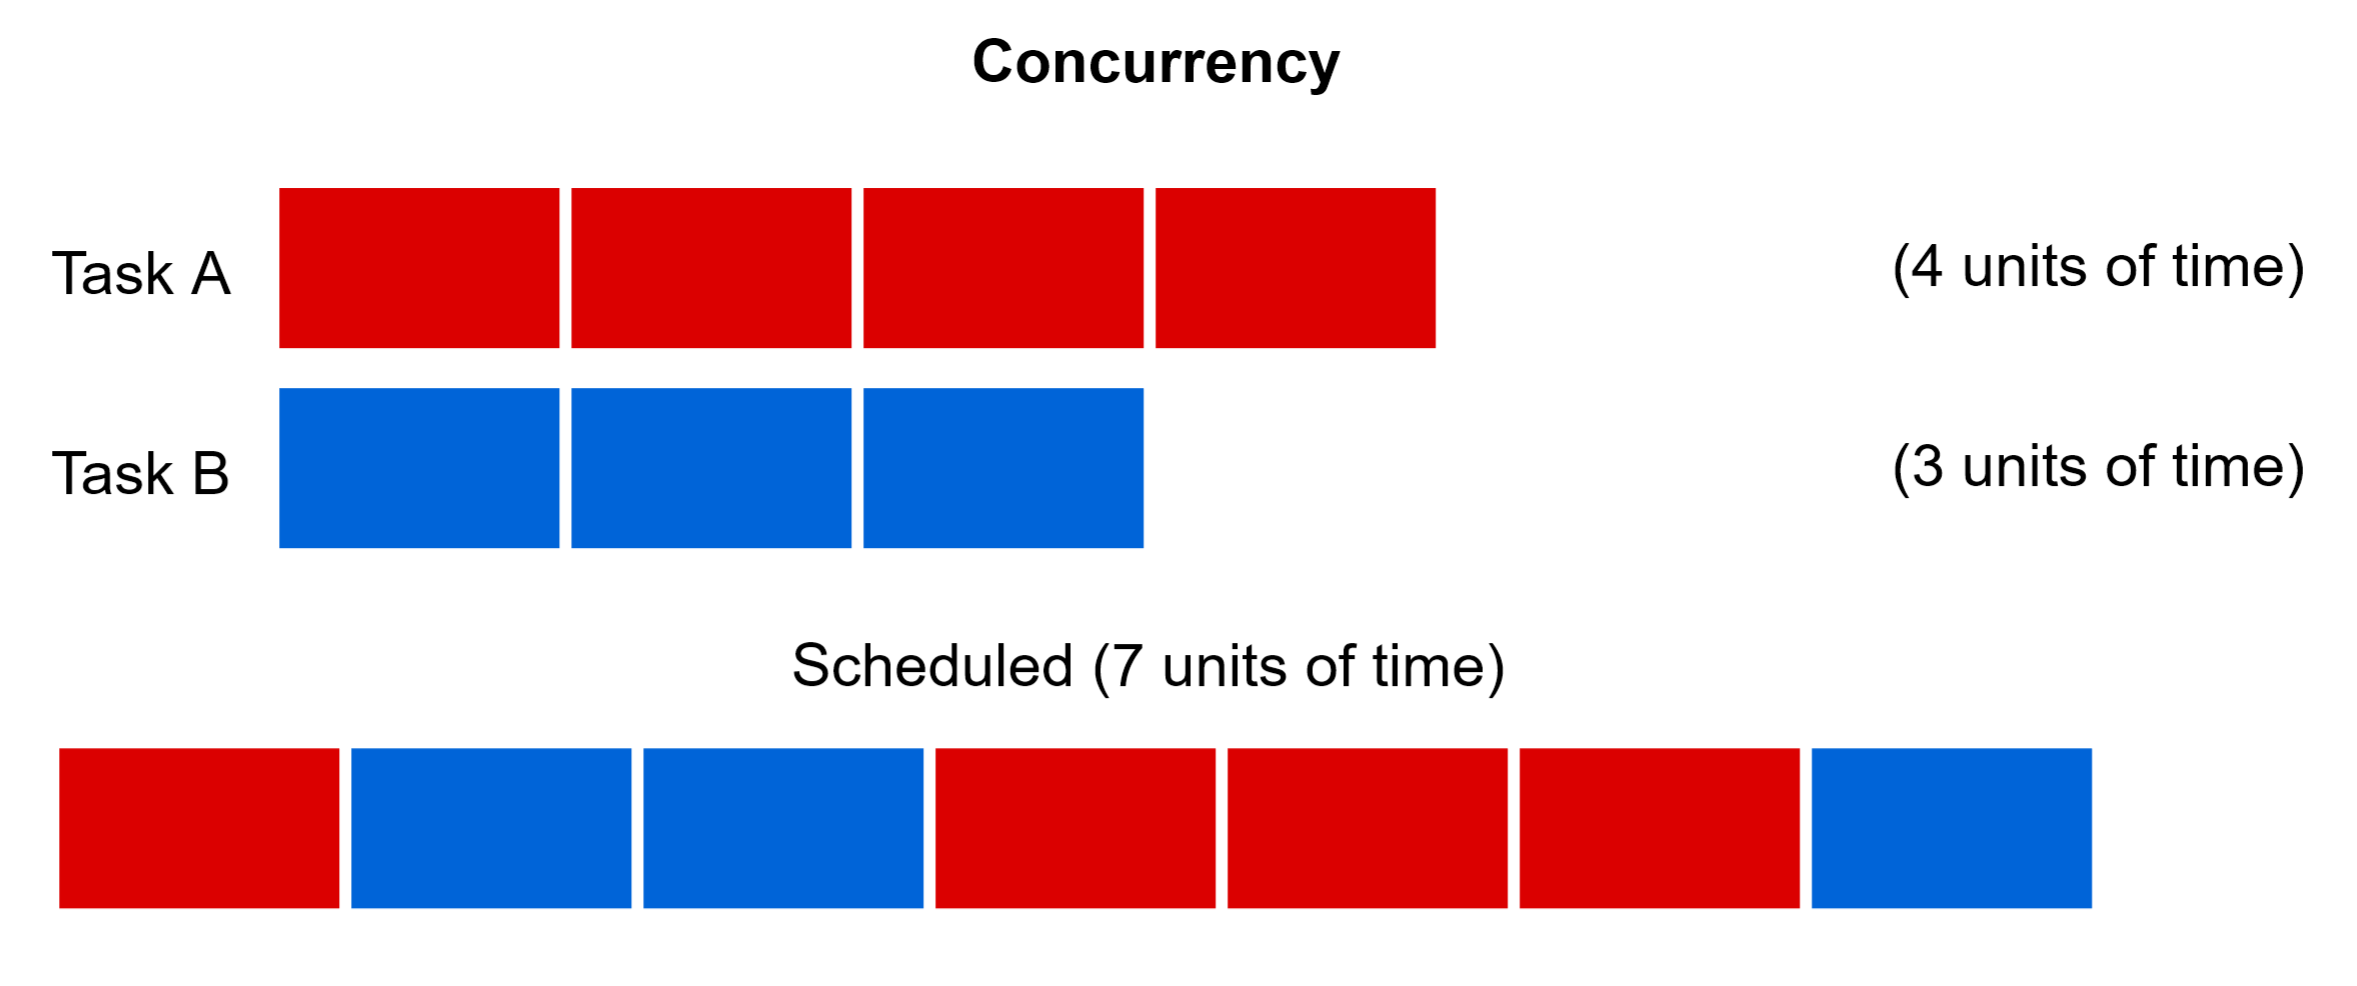
\includegraphics[width=.75\textwidth]{./Sections/high/concurrency.png}
    \caption{Concurrency: Multiple software-threads running on a single hardware-thread.}
\end{figure}

\noindent
In reality, many tasks preform I/O operations, which don't 
concern the CPU:
\begin{figure}[h]
    \centering
    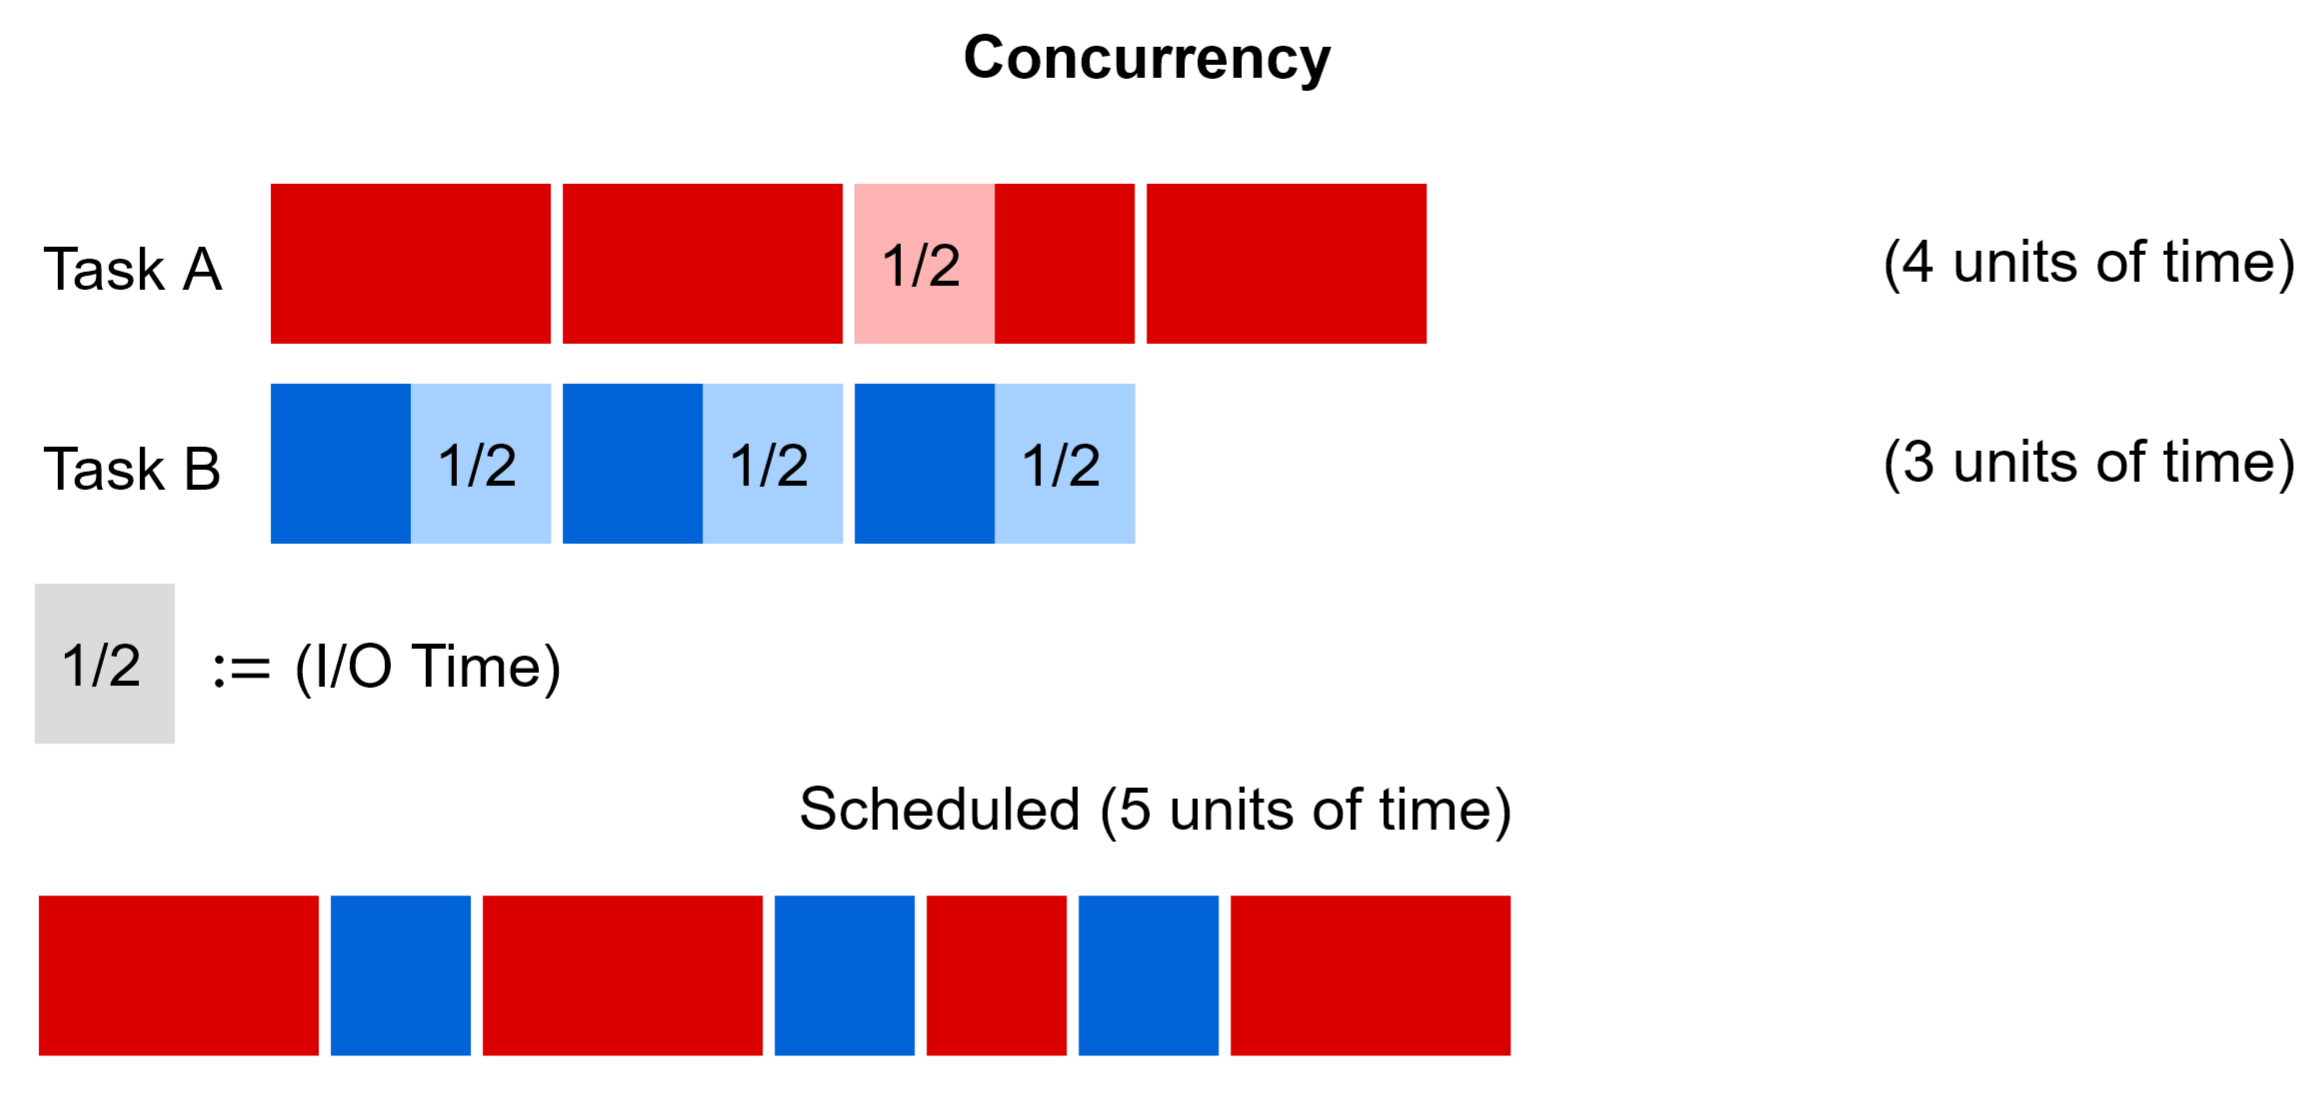
\includegraphics[width=.75\textwidth]{./Sections/high/concurrency_io.png}
    \caption{Concurrency with I/O: Multiple software-threads running on a single hardware-thread.}
\end{figure}

\noindent
Now since the CPU isn't idle on I/O operations, the overall time between tasks is cut significantly.

\newpage

\begin{Def}[Kernel]
    
    The kernel is the central component of the operating system. It manages hardware resources—including the CPU, memory, and I/O devices—and provides core services such as process management, memory management, and device control.
\end{Def}

\begin{figure}[h]
    \centering
    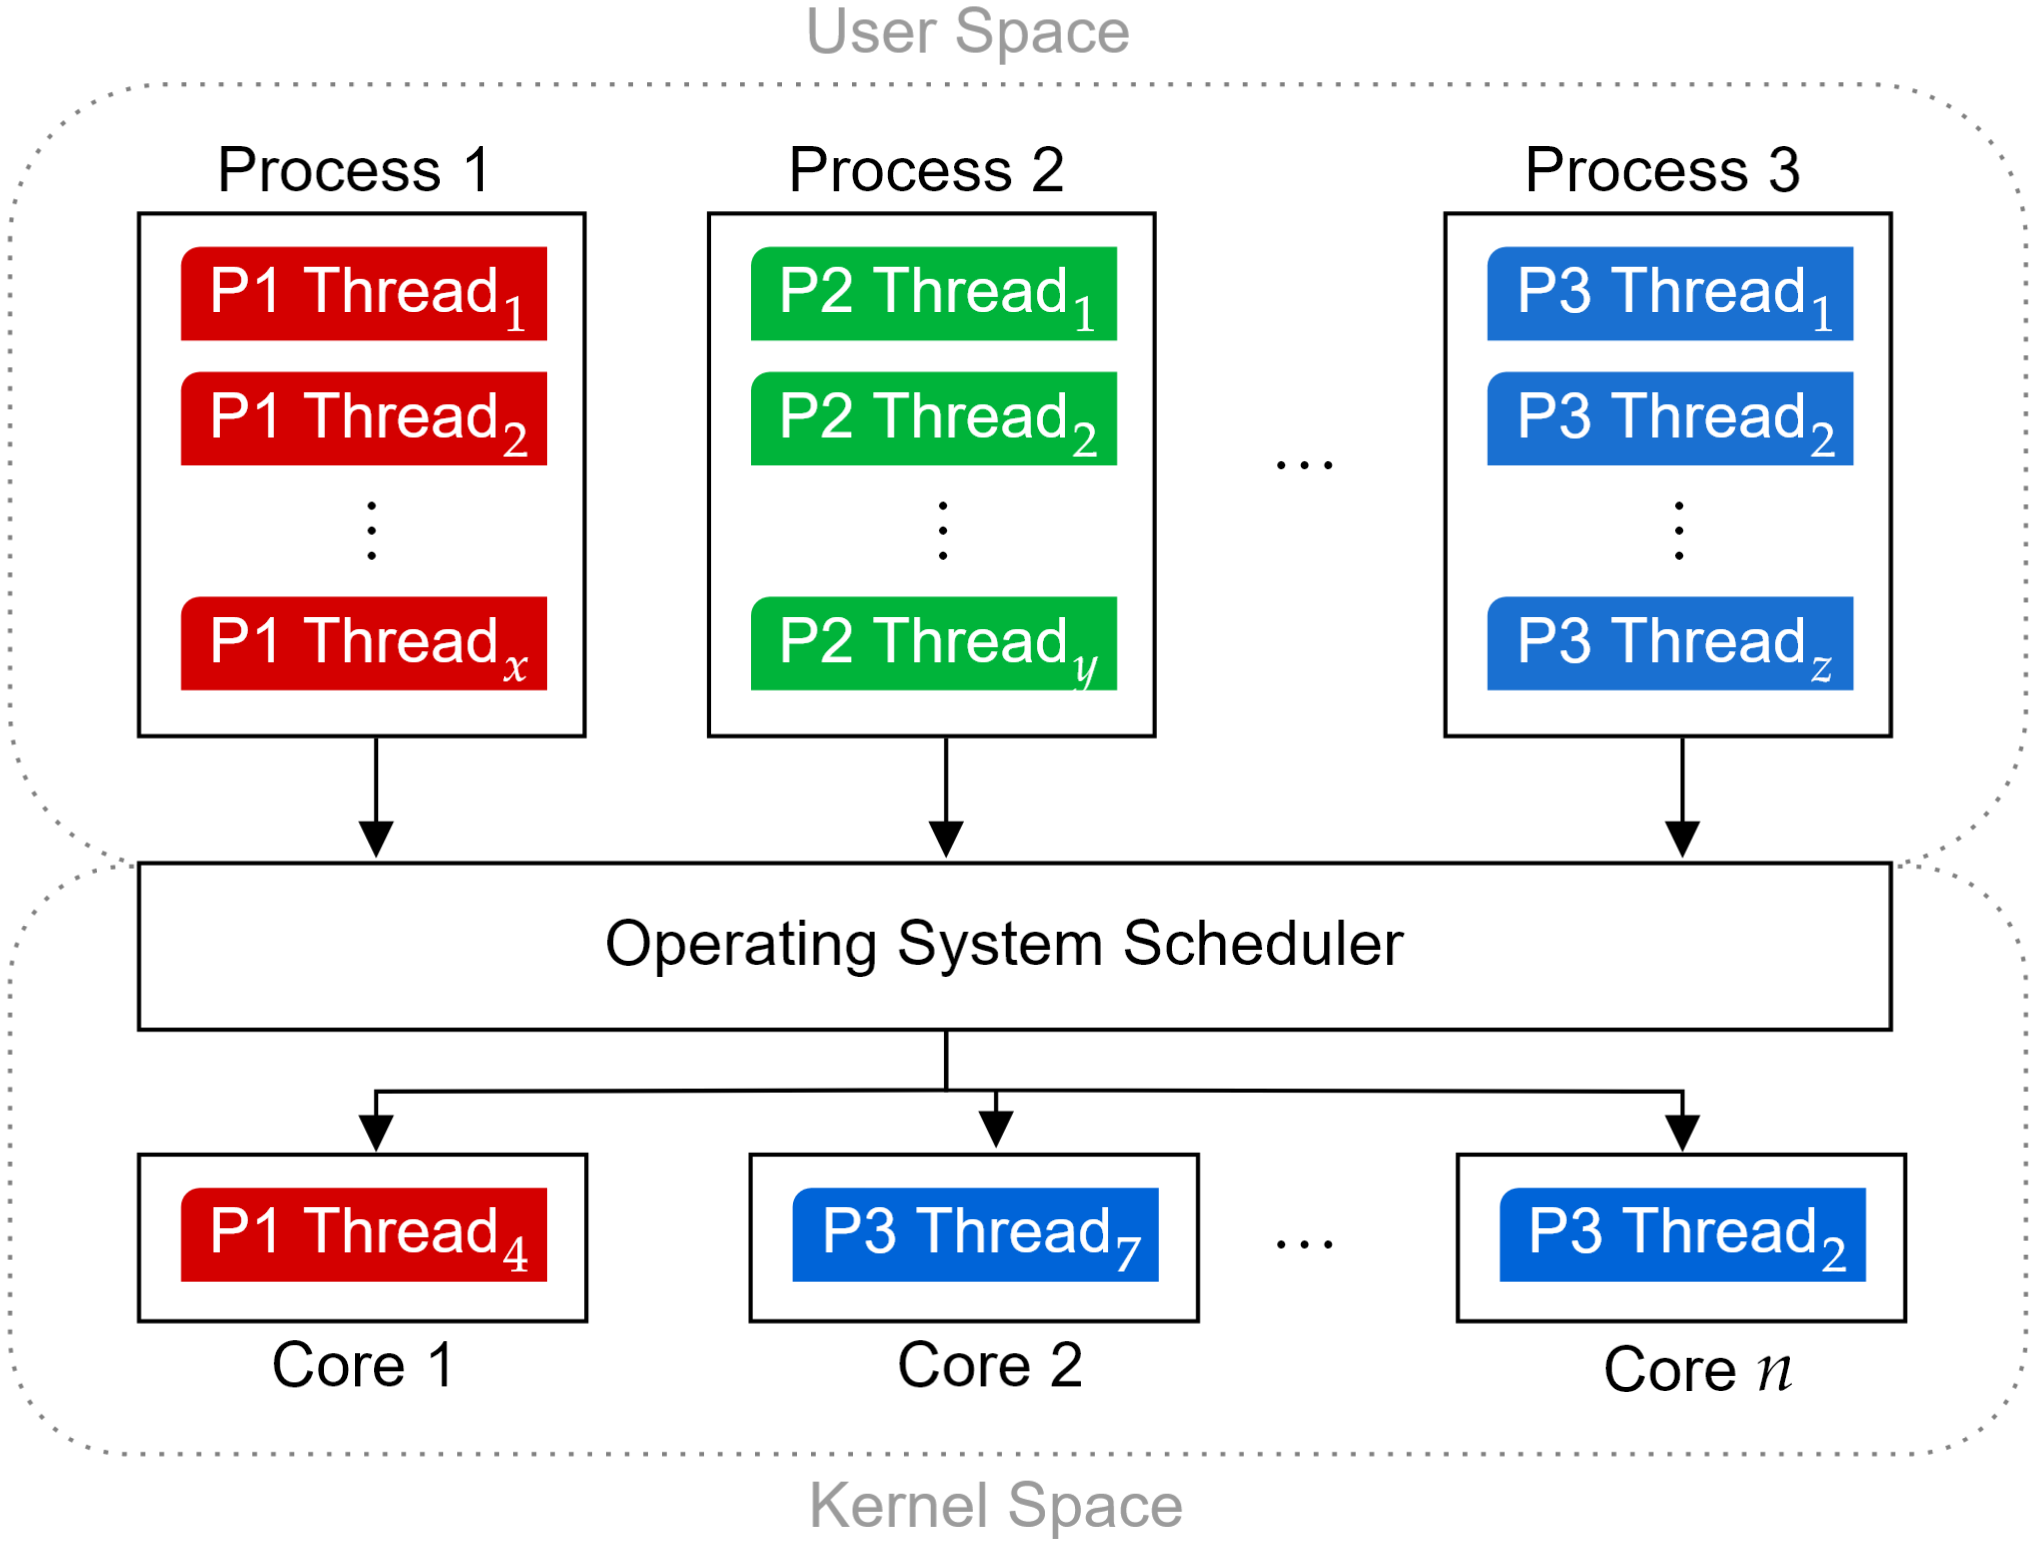
\includegraphics[width=1\textwidth]{./Sections/high/user_kernel.png}
    \caption{Process threads scheduled by the OS kernel and processed by the CPU.}
    \label{fig:kernel}
\end{figure}

\noindent
In summary, what we need to know are these key points:
\begin{itemize}
    \item The CPU executes instructions via processing units called cores/hardware-threads.
    \item The OS schedules software-threads from processes to run on hardware-threads.
    \item A core can only run one software-thread at a time, but can switch between them.
    \item Context switching on a single core is called concurrency, while utilizing multiple cores in unison (multi-threading) is called parallelism.
\end{itemize}


\newpage 

\noindent
\subsection{Motivation for Distributed Systems}

\noindent
Distributed systems cover a vast and diverse range of applications, including:
\begin{itemize}
    \item \textbf{Offloading Computation:} Perhaps a system $A$ offloads a heavy computation to system $B$.
    \item \textbf{Fault Tolerance:} If a critical system $A$ fails, an almost identical system $B$ can take over.
    \item \textbf{Load Balancing:} Say a system $A$ is overwhelmed with requests, it can distribute the load to system $B$, acting as 
    one system, from the requests point of view.
\end{itemize}
In todays market there are numerous applications of distributed systems, such as:
Cloud Computing, Social Networks, E-commerce, Streaming Services, Search Engines, Renting Computation (AI training), etc.

Let's begin to define the problem space. Say there be 
two individuals Alice and Bob, who wish to communicate:\\
\begin{figure}[h]
    \centering
    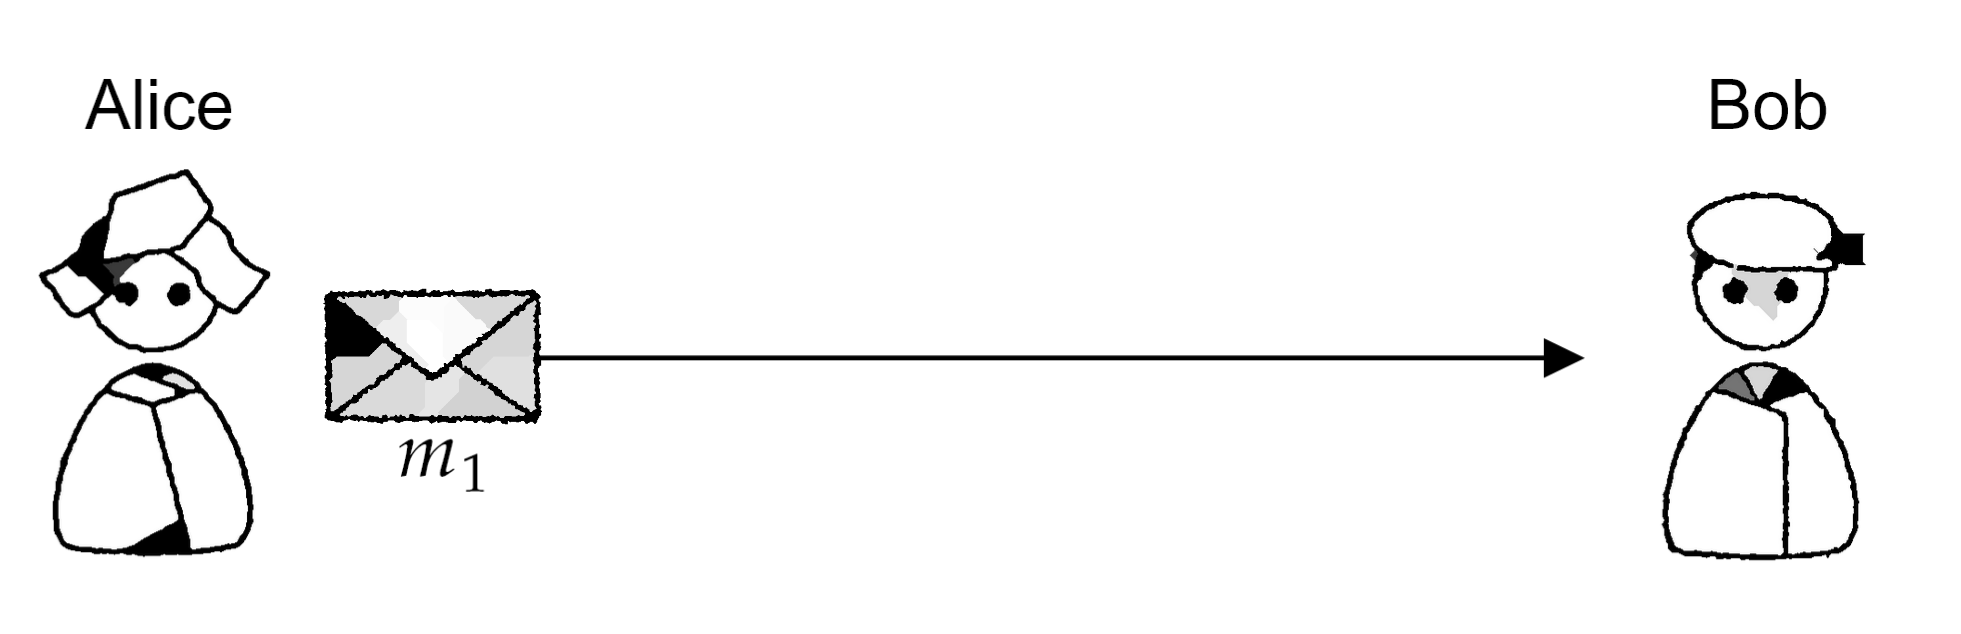
\includegraphics[width=.8\textwidth]{./Sections/high/com.png}
    \caption{Alice sends a letter $m_1$ overseas to Bob.}
\end{figure}

\noindent
How does Alice know that her message $m_1$ was received by Bob? Bob 
would have to send a message back to Alice, acknowledging the receipt of $m_1$.

\begin{figure}[h]
    \centering
    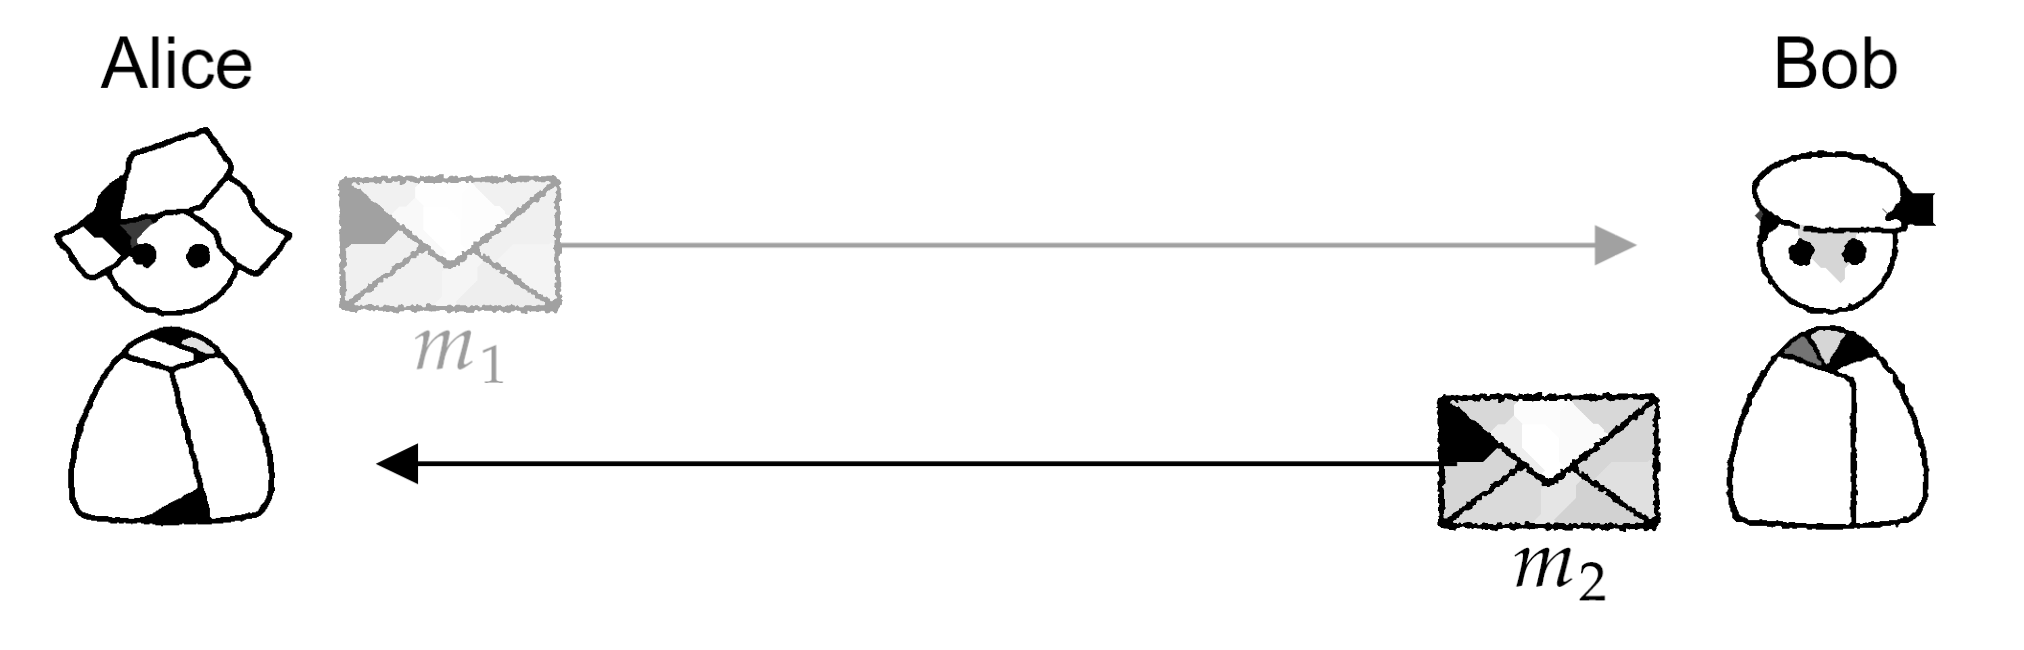
\includegraphics[width=.8\textwidth]{./Sections/high/com_2.png}
    \caption{Bob sends an acknowledgment letter back to Alice.}
\end{figure}
    
\noindent
Though problems can arise, what if Alice's letter gets lost in the mail, what if Bob receives multiple 
letters from Alice, how does Bob know which letter is the most recent? These are the fundamental problems 
of distributed systems.

% \newpage 
\section{Remote Procedure Call (RPC)}
This section will cover the concept of Remote Procedure Calls (RPCs) and how they are used in distributed systems and use the Go programming language to demonstrate such.
\subsection{Establishing a Client-Server Connection}




\begin{Def}[client-server model]

    The client-server model is a distributed application structure that partitions tasks or workloads between the providers of a
     resource or service, \textbf{called servers}, and service requesters, \textbf{called clients}. 
     
     Often clients and servers communicate over a computer network on separate hardware, but both client and server may reside in the same system.

\end{Def}

\begin{Def}[Remote Procedure Call (RPC)]

    A Remote Procedure Call (RPC) is a protocol that allows a \textbf{client} computer request the execution of functions on a separate \textbf{server} computer.

    RPC's abstract the network communication between the client and server enabling developers to write programs that may run on different machines, but appear to run locally.
\end{Def}

\begin{Def}[RPC Call Stack]

    The RPC call stack facilitates communication between two systems via four layers:
    
    \begin{enumerate}
        \item \textbf{Application Layer:} The highest layer where the client application initiates a function call. On the server side, this layer corresponds to the service handling the request.
        
        \item \textbf{Stub:} A client-side stub acts as a proxy for the remote function, \textbf{marshaling arguments} (converting them into a transmittable format) and forwarding them to the RPC library. On the server side,
        a corresponding stub, \textbf{the dispatcher}, receives the request, unmarshals the data, and passes it to the actual function.
        
        \item \textbf{RPC Library:} The RPC runtime that manages communication between the client and server, ensuring request formatting, serialization, and deserialization.
        
        \item \textbf{OS \& Networking Layer:} The lowest layer, responsible for transmitting RPC request and response messages over the network using underlying transport protocols.
    \end{enumerate}
    
    The request message travels from the client's application layer down through the stack and across the network to the server. The server processes the request in reverse, executing the function and returning the result to the client.
\end{Def}
    
\newpage 

\noindent
To illustrate the RPC call stack, observe the following diagram:
\begin{figure}[h]
    \centering
    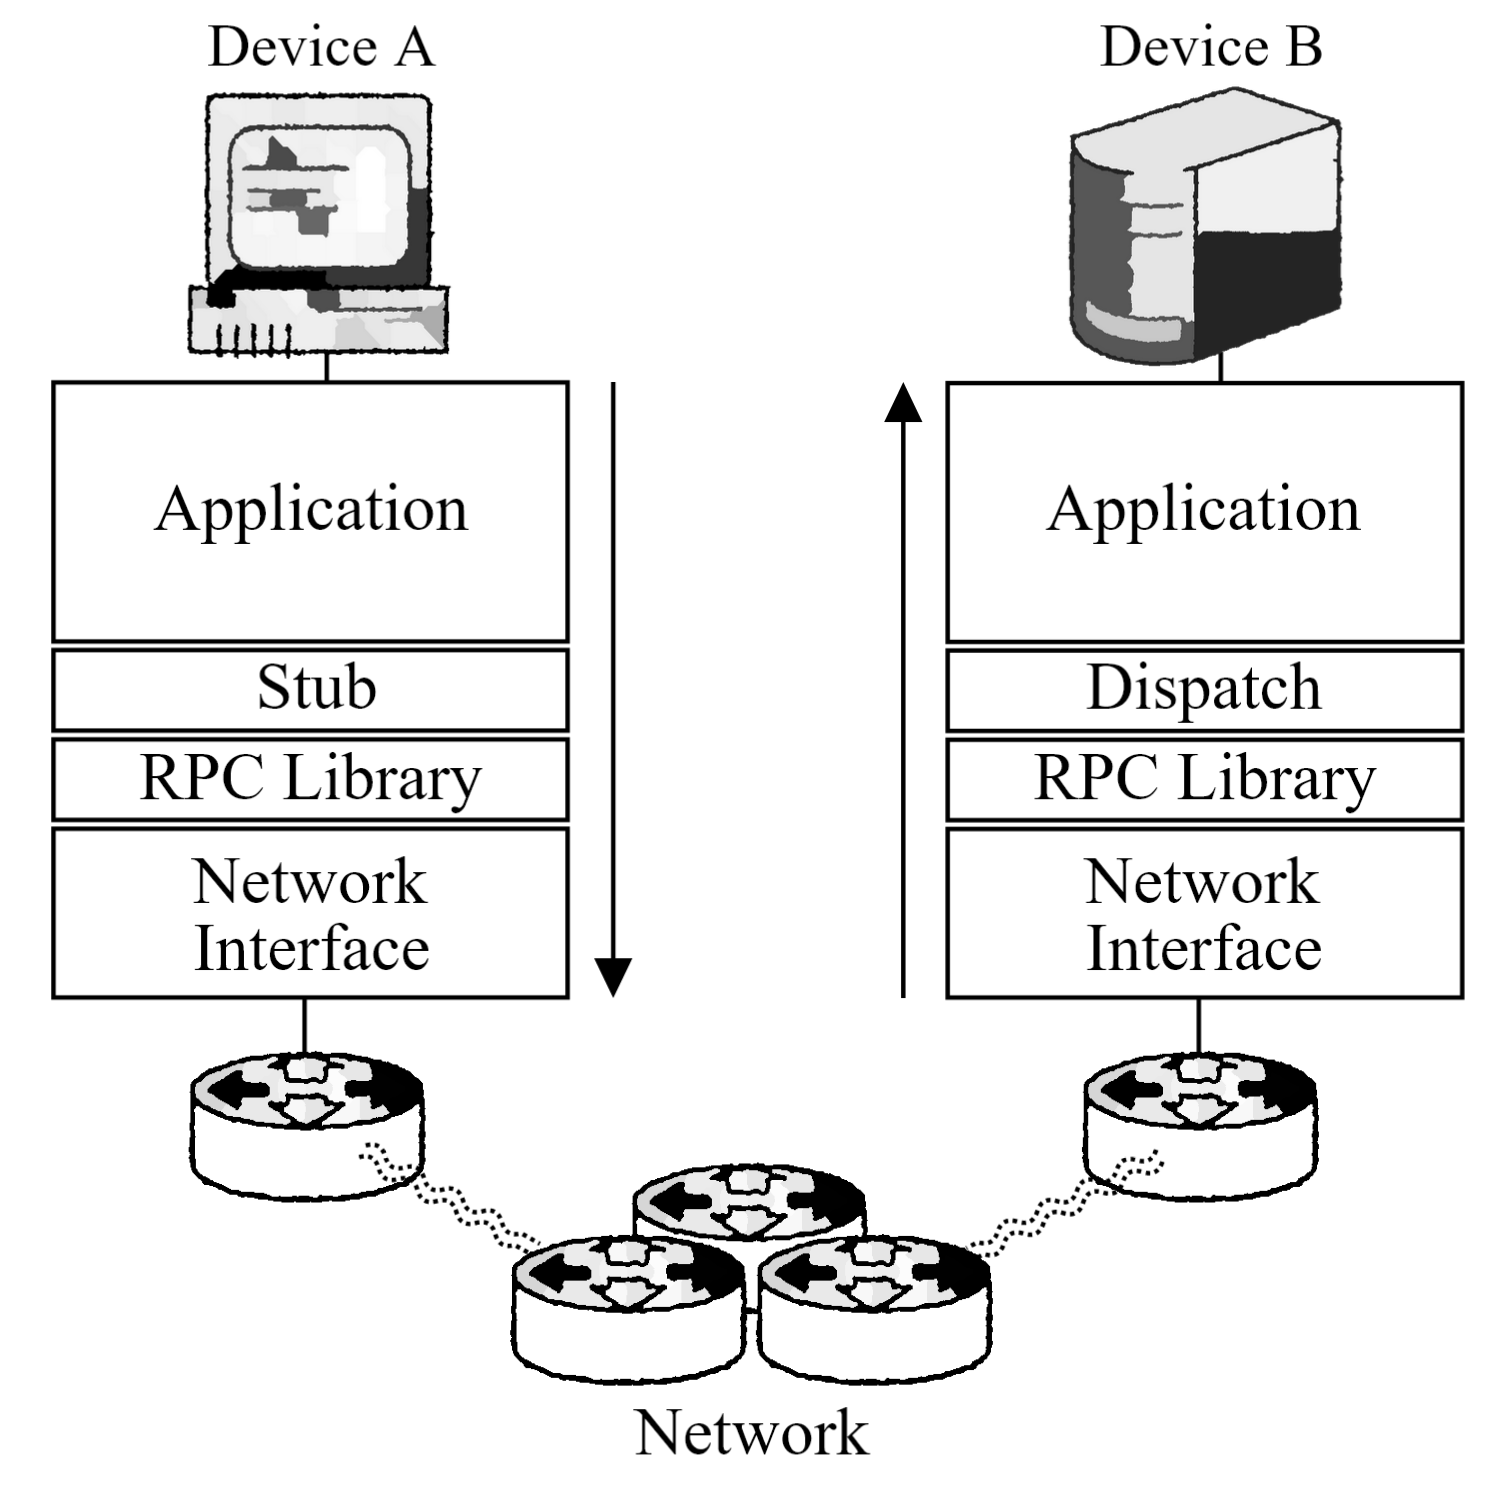
\includegraphics[width=0.55\textwidth]{Sections/rpc/rpc_stack.png}
    \caption{Client system $A$ making a request to Server system $B$ over RPC.}
    \label{fig:rpc_stack}
\end{figure}

\noindent
$B$ runs through the stub and RPC library again to reply to $A$. In terms of time it might look like:

\begin{figure}[h]
    \centering
    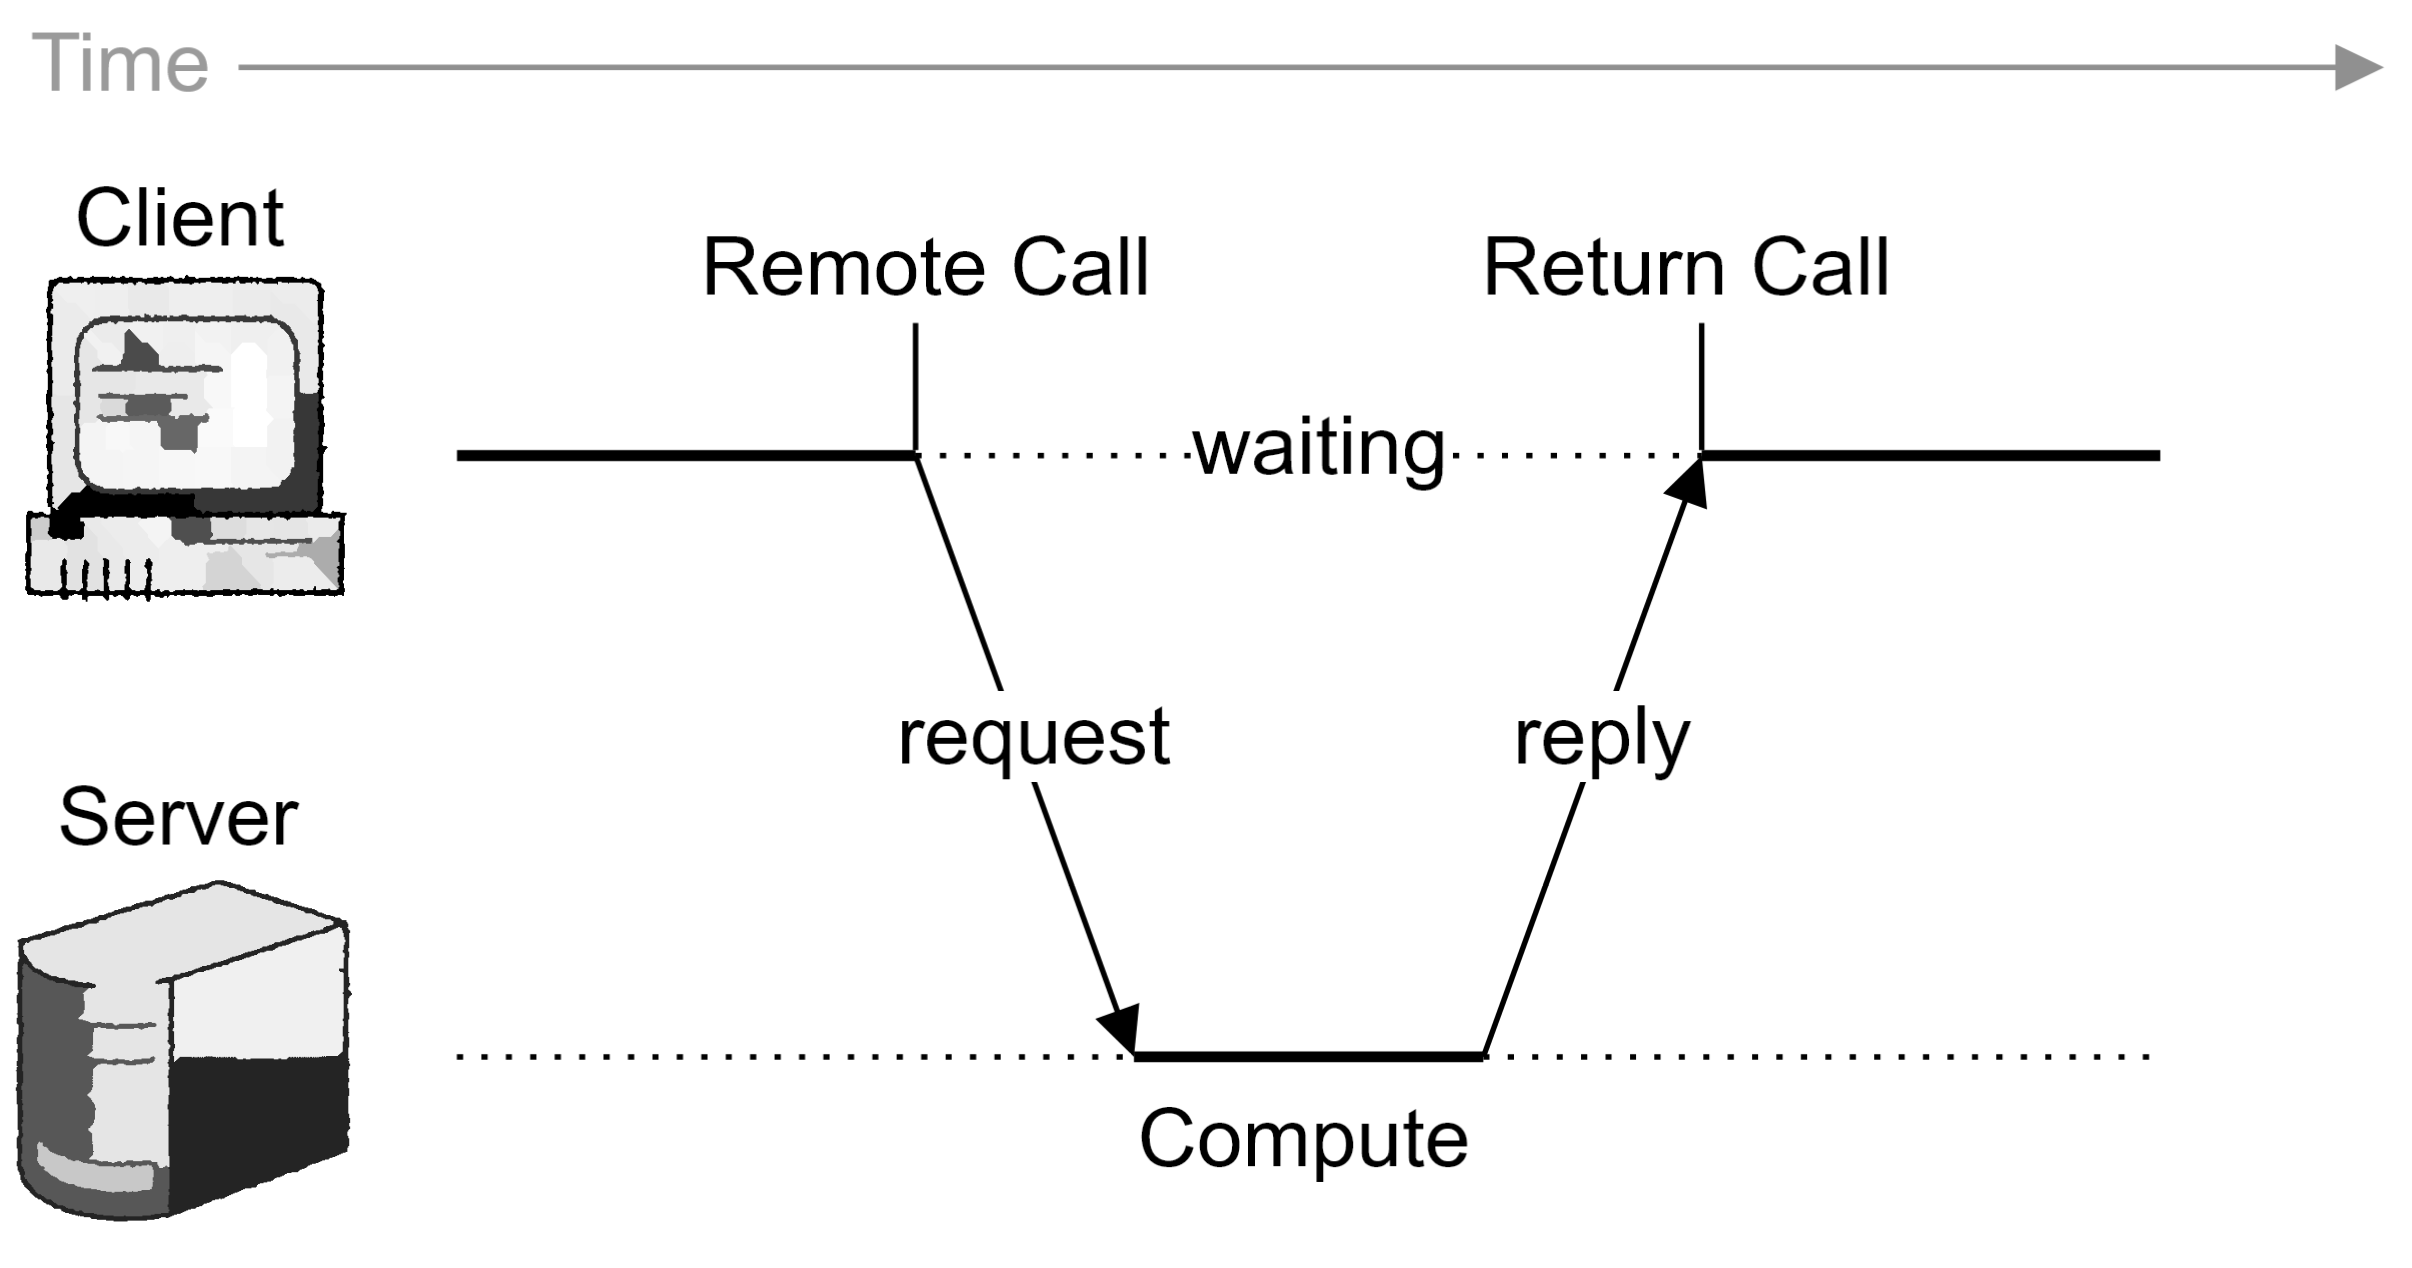
\includegraphics[width=0.63\textwidth]{Sections/rpc/call_time.png}
    \caption{RPC call stack over time.}
    \label{fig:rpc_time}
\end{figure}

\noindent 
Once the client makes the call it waits for the server to process the request and return the result. The programmer need not worry beyond sending the request and receiving the response.
The RPC deals with all the heavy work of facilitating the communication.

\newpage 

\noindent
Now to discuss what marshaling and unmarshaling are:
\begin{Def}[Marshaling and Unmarshaling]

    \textbf{Marshaling} handles data format conversions, converting the object into a byte stream (binary data).
    This conversion is known as \textbf{serialization}. This is done as the network can only transmit bytes\\
    
    \noindent
    \textbf{Unmarshaling} is the process of converting the byte stream into the original object called \textbf{deserialization}. 
    This allows the server to process the request.
\end{Def}

\noindent
To illustrate serialization and deserialization, consider the following diagram:
\begin{figure}[h]
    \centering
    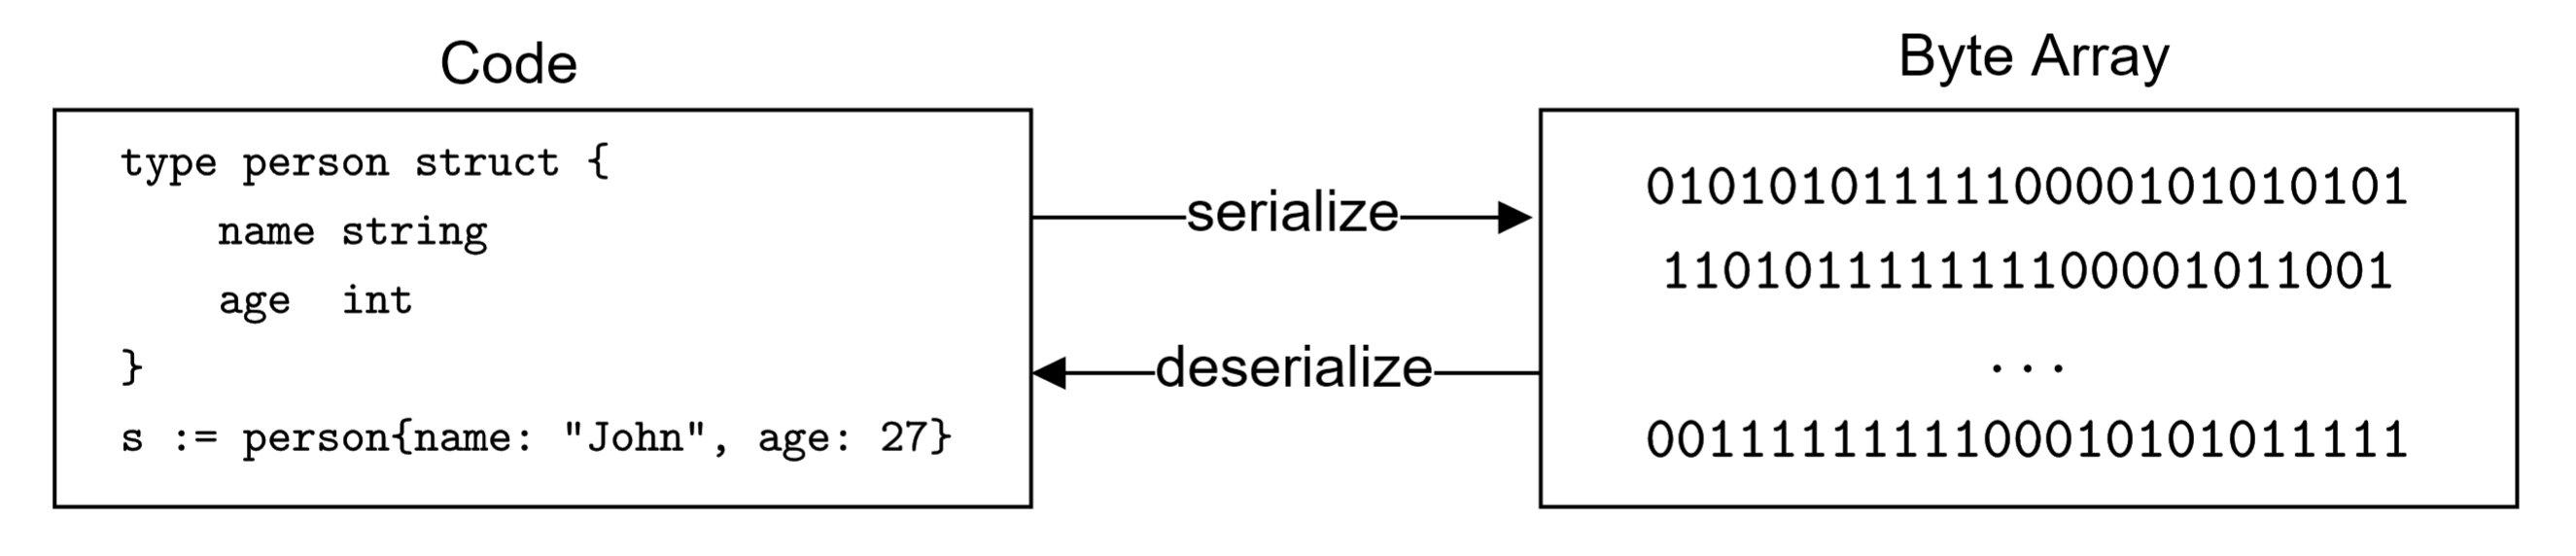
\includegraphics[width=1\textwidth]{Sections/rpc/ser.png}
    \caption{Serialization and Deserialization of data.}
    \label{fig:ser_deser}
\end{figure}

\noindent
There is one cardinal rule to remember when dealing with RPCs:
\begin{theo}[Network Reliability]

    \begin{center}
        \Large{\textbf{The network is always unreliable.}}
    \end{center}

    \vspace{1em}

    \noindent
    That is to say, the network can drop packets, delay messages, or deliver them out of order. Anything that 
    can go wrong will go wrong.
\end{theo}

\noindent
To handle network unreliability, we'll first consider two failure models:

\begin{Def}[At-least-once \& At-most-once]

    \begin{itemize}
        \item \textbf{At-least-once:} Regardless of failures, make the RPC call until the server responds. Works for read-only operations, otherwise, a strategy to handle duplicate requests is needed.
        \item \textbf{At-most-once:} Ensure the RPC call is made only once, even if the server fails to respond. This is done by having a unique identifier for each request. Each subsequent request 
        tells the server which calls have already been processed.
    \end{itemize}
\end{Def}

\newpage

\noindent
For our communication to work \textit{reliably} we need At-least-once and At-most-once with unlimited tries coupled by 
a fault-tolerant implementation. This brings us to the \textbf{GO RGC library}.

\begin{Def}[Go RPC Library]

    The Go RPC library provides a simple way to implement RPCs in the programming language Go. This gives us:
    \begin{itemize}
        \item At-most-once model with respect to a single
        client-server
        \item Built on top of single \textbf{TCP connection} (Transport Layer Protocol). This protocol ensures reliable communication between client and server.
        \item Returns error if reply is not received, e.g.,
        connection broken (TCP timeout)
    \end{itemize}
\end{Def}

\noindent
Now to discuss briefly how a basic TCP connection is made:
\begin{Def}[Establishing a TCP Connection (SYN ACK)]

    First a three-way handshake is a method used in a TCP/IP network to create a connection between a local host/client and server. 
    It is a three-step method that requires both the client and server to exchange \textbf{SYN (synchronize)}
     and \textbf{ACK (acknowledgment)}.
     \begin{enumerate}
        \item The client sends a SYN packet to the server requesting to synchronize sequence numbers.
        \item The server responds with a SYN-ACK packet, acknowledging the request and sending its own SYN request.
        \item The client responds with an ACK packet, acknowledging the server's SYN request.
     \end{enumerate}
    
    \noindent
    After the three-way handshake, the connection is established and the client and server can communicate exchanging SYN and ACK data-packets.
    To end the connection another three-way handshake takes placed, where instead of SYN, \textbf{FIN (finish)} is used.
    
\end{Def}

\noindent
Given this implementation, we approach somewhere in the realm of an \textbf{Exactly-Once model}:

\begin{Def}[Exactly-Once Model]

    The Exactly-Once model guarantees that a message is delivered exactly once to the recipient. Meaning, messages aren't duplicated, lost, or delivered out of order.
    However, In practice, data packets might do all of the above. Though with the right
    protocols in place, we can ensure order of logic is preserved.
\end{Def}

\newpage 
\noindent
Below we illustrate a simple TCP connection:
\begin{figure}[h]
    \centering
    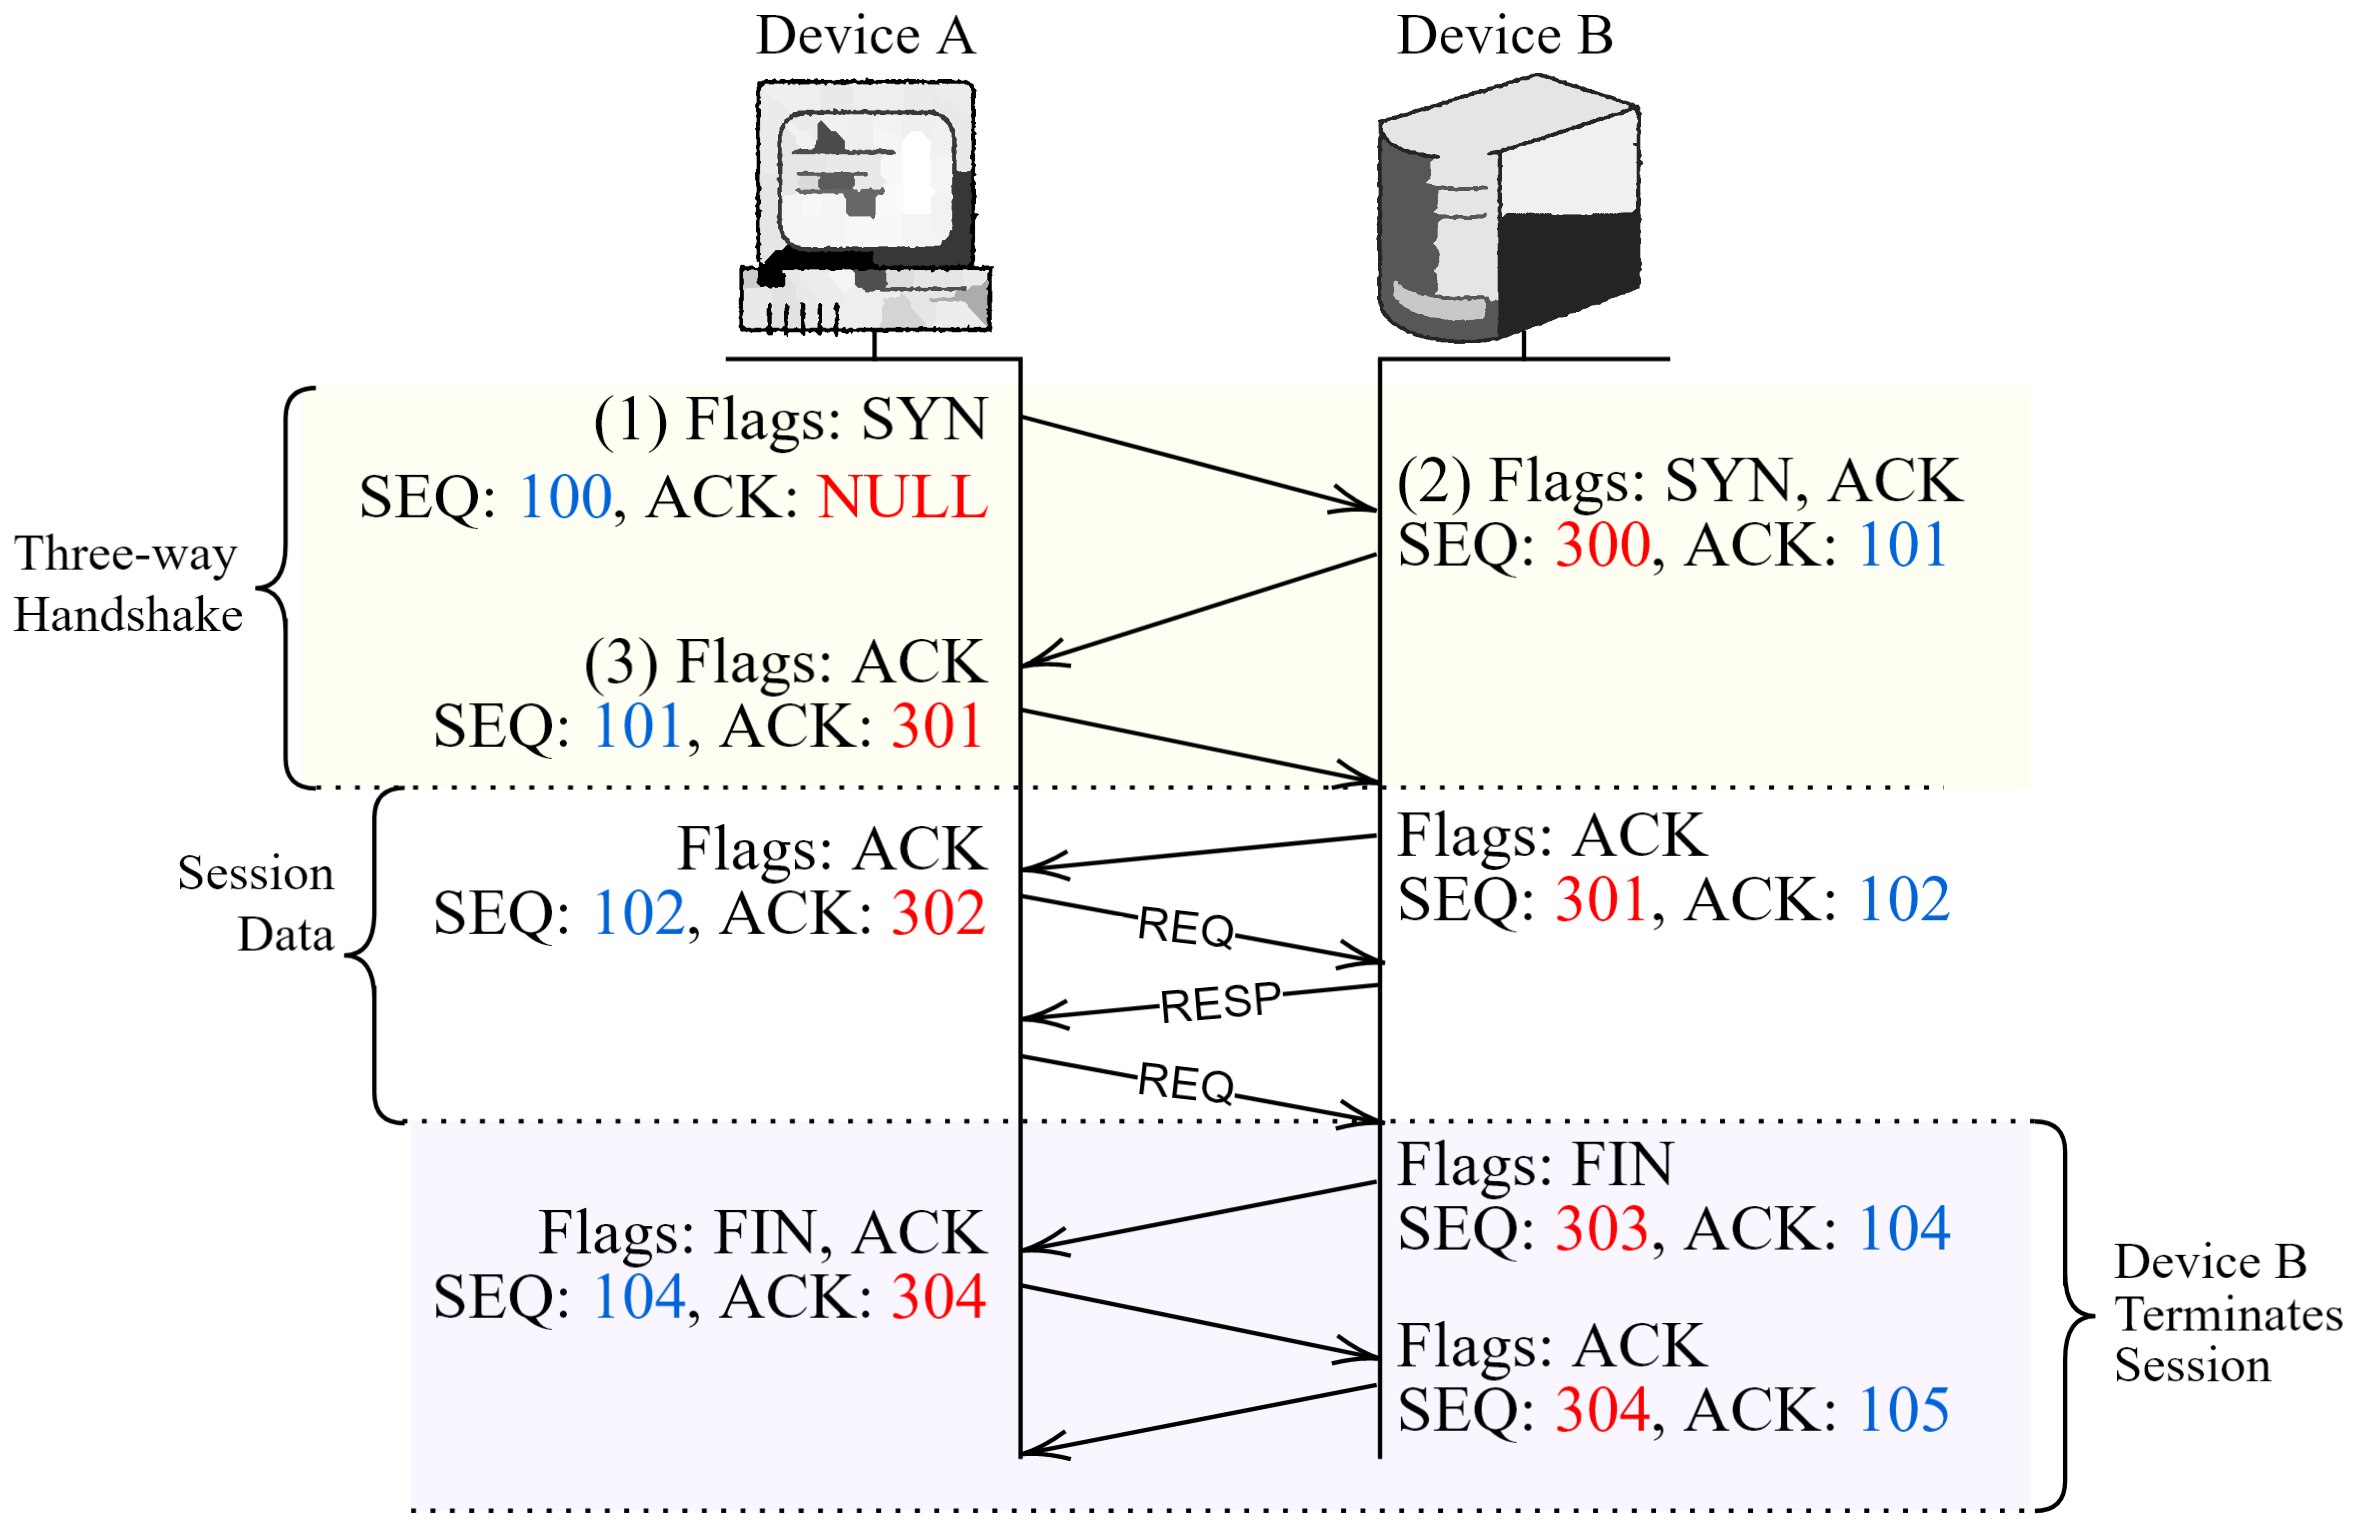
\includegraphics[width=1\textwidth]{Sections/rpc/sync.png}
    \caption{TCP Handshake, data transfer, and session termination.}
    \label{fig:tcp}
\end{figure}

\noindent
Here the client (Device A) begins a three-way handshake with the server (Device B) to establish a connection. Both start with 
arbitrary sequence numbers for security purposes. With each packet received the two devices increment their sequence numbers accordingly.\\

\begin{Tip} If there still resides curiosity for the networking aspect of RPCs, consider reading our other notes:
    \href{https://github.com/Concise-Works/Cyber-Security/blob/main/main.pdf}{https://github.com/Concise-Works/Cyber-Security/blob/main/main.pdf}
\end{Tip}

\subsection{Asynchronous Function Calls}
Let's begin to discuss how functions can run simultaneously using Go's \textbf{goroutines}:
\begin{Def}[Asynchronous Function Calls]

    An \textbf{asynchronous function call} is a function that executes independently of the main program flow, enabling tasks to run concurrently or in parallel.

\end{Def}
\newpage

\noindent
\begin{Def}[Asynchronous Function Calls in Go: Goroutines]

    A \textbf{goroutine} is a \textbf{lightweight} (lower memory overhead and scheduling cost compared to traditional OS threads)
    concurrent execution thread in Go. Goroutines enable functions to run asynchronously. Unlike traditional operating system threads, goroutines are managed by Go's runtime.
    
    A goroutine is created using the \texttt{go} keyword before a function call, signaling to the Go runtime to run the function asynchronously from the main program flow.
    
\end{Def}

\begin{Def}[Go Runtime Scheduler]

    The Go runtime scheduler is responsible for managing goroutines via three conceptual entities:
\textbf{The Go Scheduler: G, M, P}
\begin{itemize}
    \item \textbf{G (Goroutine):} A goroutine that holds the code to be executed.
    \item \textbf{M (Thread):} An OS thread that executes Go code via system calls or remains idle.
    \item \textbf{P (Processor):} Represents resources needed to execute code. The number of processors is determined by \snippet{GOMAXPROCS}.
\end{itemize}

\noindent
If there are multiple goroutines, threads, and available processors, the scheduler matches them as follows:
\begin{itemize}
    \item Many \textbf{Gs} (goroutines) are mapped to available \textbf{Ms} (OS threads), which execute them using \textbf{Ps} (processors) as execution resources.
\end{itemize}

\noindent
\textbf{Queues in the Scheduler}
\begin{itemize}
    \item \textbf{Global Run Queue (GRQ):} Holds all new goroutines that are yet to execute.
    \item \textbf{Local Run Queue (LRQ):} Holds goroutines that are assigned to a specific \textbf{P}.
\end{itemize}

\noindent
For example, let the processors in the scheduler be defined as 
$
P = \{ P_1, P_2, \dots, P_n \}
$
where \( n = \texttt{GOMAXPROCS} \). Then the scheduler follows the following steps:
\begin{enumerate}
    \item If \( P_1 \) has no more goroutines to execute, it follows these steps:
    \begin{enumerate}
        \item Check \textbf{GRQ} for a \textbf{G} (goroutine) roughly \textit{1/61th of the time}.
        \item If nothing is found, check \textbf{LRQ} again.
        \item If nothing is found, attempt to \textbf{steal} work from other \textbf{Ps}.
        \item If nothing is found, check \textbf{GRQ} one last time.
        \item Finally, \textbf{poll the network} (i.e., check for incoming network work).
    \end{enumerate}
\end{enumerate}
\end{Def}

\newpage
\noindent
To illustrate the Go runtime scheduler on a high-level, consider the following diagram in contrast to Figure \ref{fig:kernel}: 

\begin{figure}[h]
    
    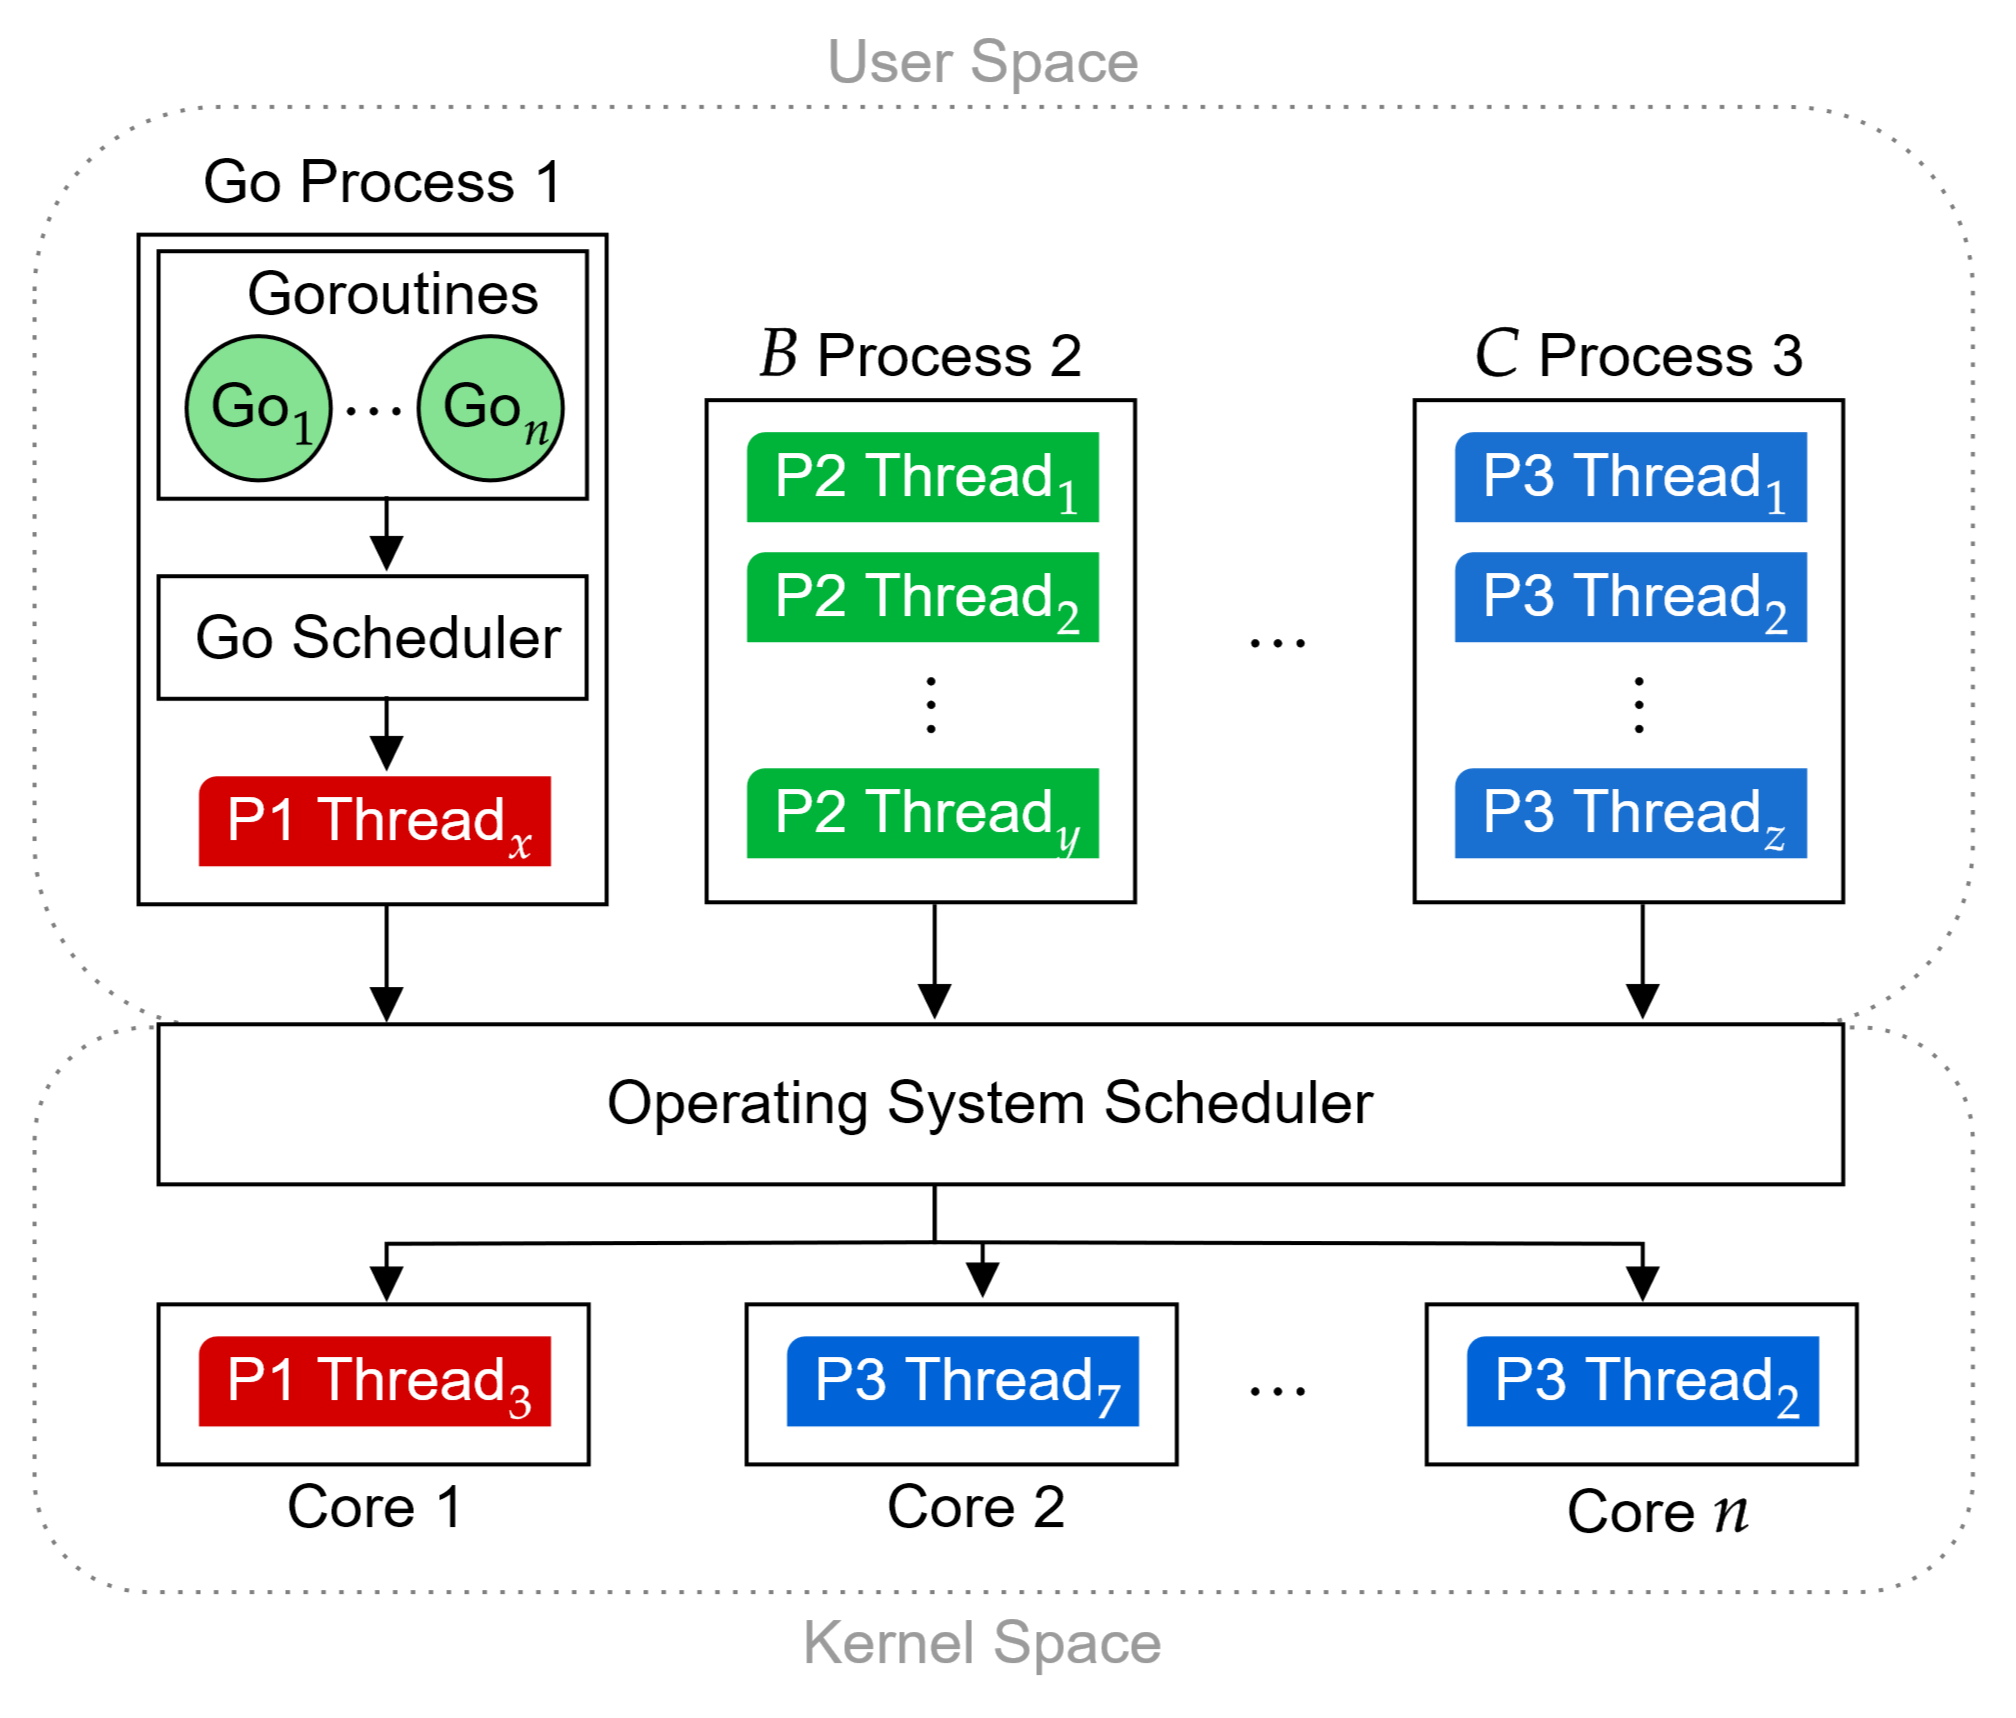
\includegraphics[width=1\textwidth]{Sections/rpc/high_sched.png}
    \caption{Go runtime scheduler with G, M, P entities.}
    \label{fig:go_scheduler}
\end{figure}
\noindent
Where the system has many different processes $B$, $C$ and so on, we focus on the process that contains an instance of the Go runtime scheduler.
Within this process each goroutine is scheduled by the Go runtime scheduler. The Go scheduler determines the number of threads needed
and assigns goroutines to them. The process then presents these threads to the OS Scheduler which assigns them to the available cores.

In particular, \textbf{The OS has the final decision on which threads run on which cores.} The Go runtime scheduler only manages what threads to present.
This is still helpful as the Go runtime can context switch the threads between goroutines before the handoff. Hence, the name \textbf{lightweight threads}, as 
context switching for the OS is expensive.

\newpage 
\noindent
In particular we zoom in on the Go runtime scheduler of a single process: 
\begin{figure}[h]
    
    \hspace{-5em}
    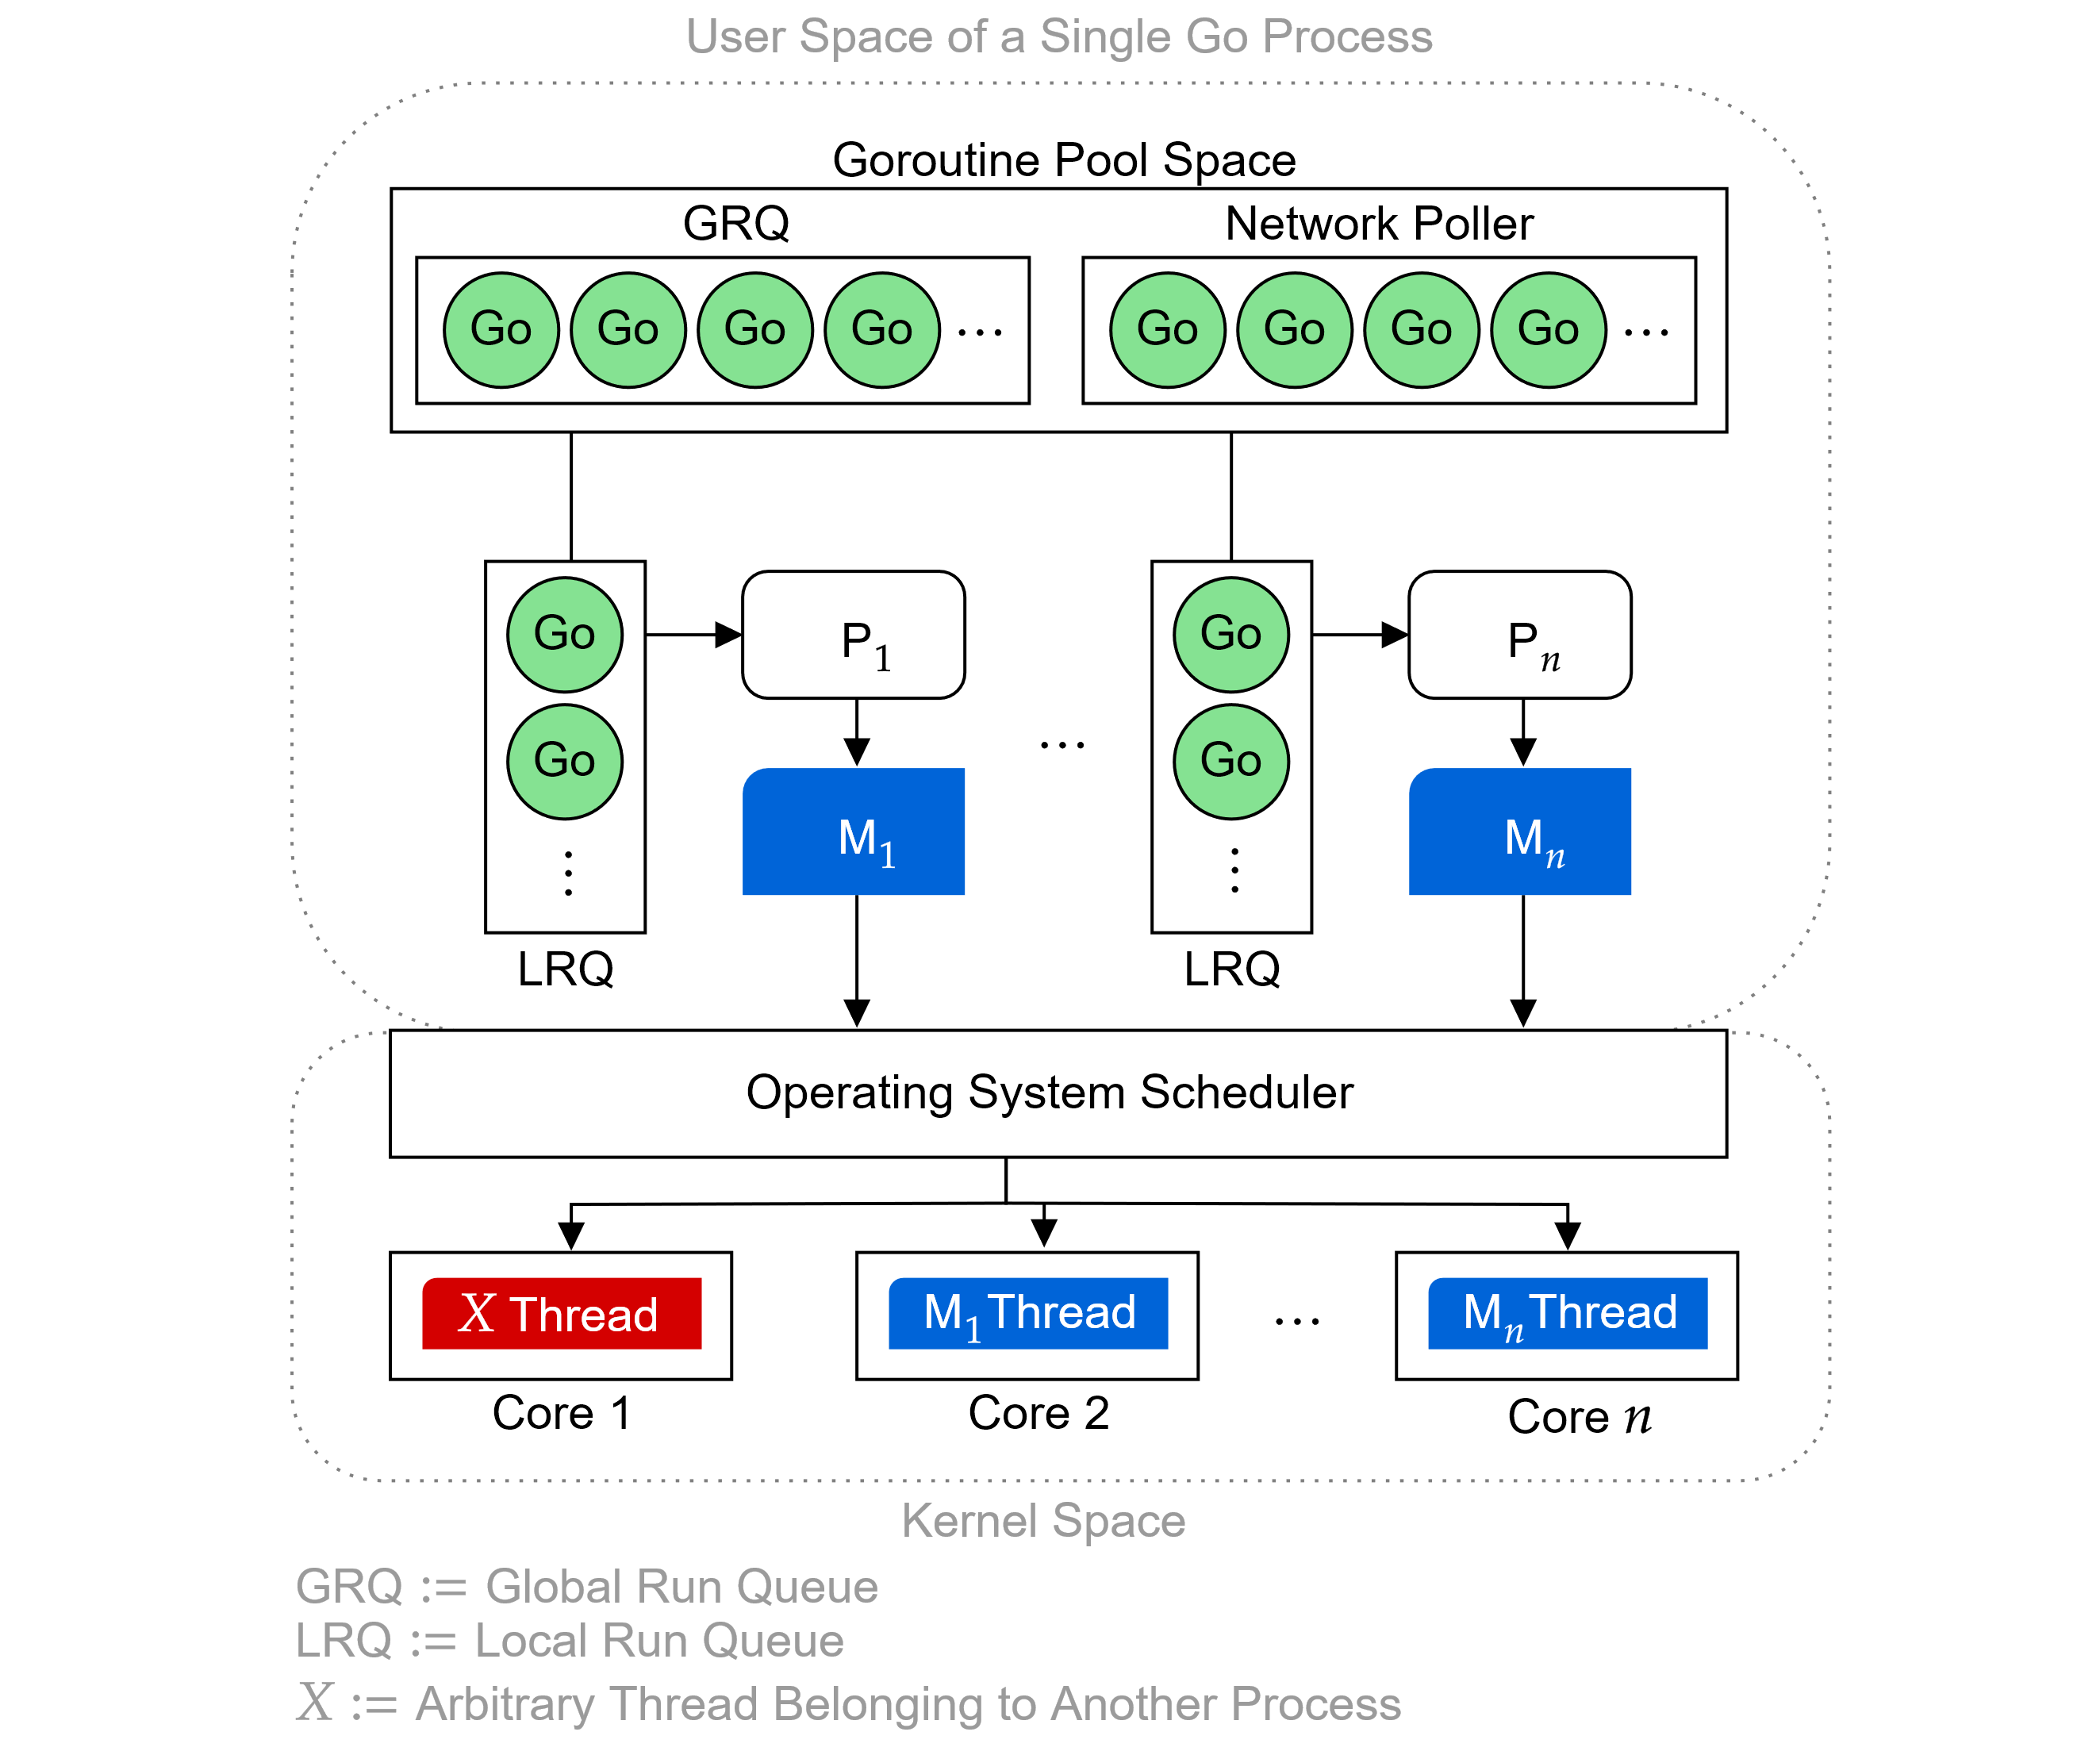
\includegraphics[width=1.1\textwidth]{Sections/rpc/sheduler.png}
    \caption{Go runtime scheduler within a single process.}
    \label{fig:scheduler}
\end{figure}

\noindent
Here our ``Goroutine Pool Space'' represents the latent goroutines waiting to be executed. 
We populate the LRQs of each P and their assigned M thread. The Ms are presented to the OS Scheduler. Moreover, 
the $X$ is some arbitrary thread belonging to another process on the system.\\
For emphasis
\begin{theo}[Go Runtime Scheduler vs. OS Scheduler]

    The Go runtime only manages threads to present; The OS schedules threads to cores.
\end{theo}
\newpage 

\noindent
In all, the asynchronous nature of goroutines may create undefined behavior if not handled properly.
\begin{Example}[Count to n using Goroutines]

    \label{ex:goroutine}
    Consider the following Go program that counts to $n$ using a goroutine:
    \begin{lstlisting}[language=Go, caption=Goroutine Example: Count to n, label={lst:goroutine}, numbers=none]
    package main // Required for Go programs to run as executables
    import (
        "fmt"
        "time"
    ) // Import required packages : fmt for printing and time for sleep
    
    // ''i:=1'' is short for ''var i int = 0''
    func countUp(n int) {
        for i := 1; i <= n; i++ {
            // Anonymous function declared as a goroutine
            go func() {
                fmt.Println("Goroutine:", i)
            }()
        }
    }
    // Main entry point of the program
    func main() {
        countUp(5)
    }
    \end{lstlisting}
    \noindent
    However, this won't print anything as the main function exits before the independent goroutine can finish. A simple fix we'll do for now is put a sleep to wait for the goroutine to finish.
    \begin{lstlisting}[language=Go, caption=Adding a Sleep to Wait for Goroutine, label={lst:sleep}, numbers=none]
        func main() {
            countUp(5) // contains a goroutine
            time.Sleep(2 * time.Second) // Wait for goroutine to finish
            fmt.Println("Main function exits")
        }
    \end{lstlisting}

    Ensuring the main function waits for the goroutine to finish.
\end{Example}

\begin{theo}[Main Goroutine Thread]

    the main function of a goroutine is too a kind of goroutine. We may refer to it as the \textbf{main goroutine} or \textbf{main thread}.
    In particular, the main goroutine is the first to run and may finish before any other goroutine.
\end{theo}


\newpage 

\noindent
Though since calls happen independent of each other means they happen simultaneously.
\begin{Example}[Count to n using Goroutines Corollary]

    \label{ex:goroutine_corollary}
    Continuing off from the previous example (\ref{ex:goroutine}), we'll get an output such as:
    \begin{lstlisting}[language=Go, caption=Output of Goroutine Example, label={lst:output}, numbers=none]
    ...
    func countUp(n int) {
        for i := 1; i <= n; i++ {
            go func() {
                fmt.Println("Goroutine:", i)
            }()
        }
    }

    func main() {
        countUp(5) // Runs countUp concurrently
        time.Sleep(2 * time.Second) // Wait for goroutine to finish
        fmt.Println("Main function exits")
    }

    /* Output:
    Goroutine: 4
    Goroutine: 3
    Goroutine: 5
    Goroutine: 2
    Goroutine: 1
    Main function exits
    */
    \end{lstlisting}
    \noindent
    The goroutine spawns multiple threads for each print of counter $i$. Therefore the order at which they execute is 
    up to the Go runtime scheduler.
\end{Example}

\begin{theo}[Goroutines and Multithreading]

    Goroutines will attempt to run on multiple threads to achieve parallelism. However, if there isn't enough cores available, 
    threads will run concurrently on the same core.

    To declare how many cores can use, \snippet{runtime.GOMAXPROCS} from the \snippet{runtime} package can be used.
    \begin{lstlisting}[language=Go, caption=Setting the Number of Cores for Goroutines, label={lst:cores}]
        import "runtime"
        runtime.GOMAXPROCS(n) // n = number of cores to use
    \end{lstlisting}
    \noindent
    By default, Go will use the number of cores available on the machine.
\end{theo}

\newpage 

\noindent
Try these examples out in Go to get a feel for how goroutines work.

\begin{Def}[Installing and Running Go Programs]

    First, install Go from the official website: \href{https://go.dev/doc/install}{https://go.dev/doc/install}.
    The Go file extension is \snippet{.go}:
    \begin{itemize}
        \item \textbf{To run a Go program:} Use the command \snippet{go run <filename>.go}.
        \item \textbf{To build a Go program:} Use the command \snippet{go build <filename>.go} to create an executable.
        Then run the program in a terminal via \snippet{./<filename>}.
    \end{itemize}
\end{Def}

\begin{Tip}
    This text will teach the necessary components as we go along. However, if one wishes to learn on their own 
    a little first, consider the following resource: \href{https://gobyexample.com/}{https://gobyexample.com/}.
    Though this text does assume prior programming knowledge and should be follow-able without the resource.
\end{Tip}
\subsection{Synchronization: Data Races \& Deadlocks}
\noindent
Asynchronous functions introduces a problem: If two threads access the same memory location at the same time,
we face corruption of data as they try to write over each other:
\begin{Def}[Data Race]

    A \textbf{data race} occurs when multiple threads or goroutines access the same memory location concurrently, and at least one of the accesses is a write operation, without proper synchronization. This leads to undefined behavior, including inconsistent data and unpredictable program execution.
    \end{Def}
        
\noindent
To avoid data races we implement the following strategy:
\begin{Def}[Mutex (Mutual Exclusion)]

    A \textbf{mutex} (short for \emph{mutual exclusion}) is a synchronization primitive that prevents multiple threads from simultaneously accessing shared resources. This allows a single thread to place a \textbf{lock} on the resource, ensuring exclusive access until the lock is released.
\end{Def}

\newpage
    
\noindent
Go has their own mutex implementation:
\begin{Def}[Go Mutex]
    
    In Go, the \snippet{sync.Mutex} type provides a way to control access to shared data. A \texttt{Mutex} has two main methods:
    \begin{itemize}
        \item \snippet{Lock()}: declares that the current goroutine from which it resides has exclusive access to the resource.
        \item \snippet{Unlock()}: Releases the mutex, allowing other goroutines to access the resource.
    \end{itemize}
\end{Def}
    
\vspace{-.5em}
\begin{Example}[Increasing a Counter Variable with Goroutines]

    \label{ex:counter}
    Consider the following example where a function \snippet{incCounter()} increments a shared counter variable:
    \begin{lstlisting}[language=Go, caption=Incrementing a Counter Variable, label={lst:counter}, numbers=none]
    ...
    var counter int // declaring global counter variable
    
    func incCounter() {
        counter = counter + 1
    }

    func main() {
        // forloop spawning an instance of incCounter() in a goroutine
        for i := 0; i < 1000; i++ {
            go func() {
                incCounter()
            }()
        }
        time.Sleep(5 * time.Second)
        fmt.Println("Counter:", counter)
    }
    /* Output: Counter: 982 */
    \end{lstlisting}
    \noindent
    By the end of the forloop, the counter will most often not be 1000. This is due to counter having 
    a different state in each goroutine. To fix this, we'll use a mutex. So it is very possible that the first 2 goroutines 
    look like this:
    \begin{itemize}
        \item Goroutine 1: \snippet{counter = 0 + 1}
        \item Goroutine 2: \snippet{counter = 0 + 1}
    \end{itemize}
    \noindent
    Where all three goroutines see the counter as 0, increment it all setting it to 1.
\end{Example}

\newpage 

\noindent
Now to fix the previous example (\ref{ex:counter}) using a mutex:

\begin{Def}[Increasing a Counter Variable with a Mutex]

    To ensure a global variable counter is incremented correctly, we'll use a mutex:
    \begin{lstlisting}[language=Go, caption=Using a Mutex to Increment a Counter Variable, label={lst:mutex}, numbers=none]
    ... // imported the "sync" package for the mutex
    var counter int
    var mu sync.Mutex // declaring a mutex

    func incCounter() {
        mu.Lock() // Lock the mutex
        counter = counter + 1
        mu.Unlock() // Unlock the mutex
    }

    func main() {
        for i := 0; i < 1000; i++ {
            go func() {
                incCounter()
            }()
        }
        time.Sleep(5 * time.Second)
        fmt.Println("Counter:", counter)
    }

    /* Output:
    Counter: 1000
    */
    \end{lstlisting}

    \noindent
    By using a mutex, we ensure that only one goroutine can access the shared counter variable at a time.
    \underline{\textbf{Important Note:} This does not ensure the order in which the goroutines run.}
\end{Def}

\noindent
Though with mutexes may come another problem, what if a goroutine never releases the lock?
\begin{Def}[Deadlock]

    A \textbf{deadlock} occurs when two or more asynchronous processes are waiting for each other to release a resource, preventing all processes from progressing. This results in a program that hangs indefinitely.
\end{Def}
\noindent
In a large project a logical mistake in a sea of processes can lead to a deadlock. 

\newpage

\noindent
\begin{Example}[Deadlock Scenario]
    
    Say we have functions \snippet{task1()} and \snippet{task2()} that each require a mutex lock:
    \begin{lstlisting}[language=Go, caption=Deadlock Scenario, label={lst:deadlock}, numbers=none]
    ... // dots represent some passage of code

    go func task1() {
        lockA.lock() ... lockB.lock()
        ...
        lockB.unlock() ... lockA.unlock()
    }

    go func task2() {
        lockB.lock() ... lockA.lock()
        ...
        lockA.unlock() ... lockB.unlock()
    }
    
    ...
    \end{lstlisting}
    Depending on how the scheduler runs, these two tasks will lock each other out, halting the program indefinitely.
\end{Example}


\subsection{References \& Pointers in Go}

\noindent
In Go, problems may arise from how Go deals with scoped variables:
\begin{Def}[Reference vs. Value Types]

    In Go, variables can be either \textbf{reference types} or \textbf{value types}:
    \begin{itemize}
        \item \textbf{Reference Types:} Point to a memory location where the actual data is stored. Changes to the reference type will affect all variables pointing to the same memory location.
        \item \textbf{Value Types:} Store the actual data in memory. Changes to a value type will not affect other variables.
    \end{itemize}
\end{Def}

\begin{Def}[Closures and Reference Types]

    In Go, if a variable isn't explicitly pass to a function, but is rather accessible from the function's scope, it is considered a \textbf{closure}. This 
    closure is a reference to the variable, not the data itself.
\end{Def}

\newpage 

\begin{Example}[Closures and Goroutines]

    Let \snippet{data} be some channel and \snippet{do\_something()} be some function that returns a value:

    \begin{lstlisting}[language=Go, numbers= none]
    ...
    batch := 0
    for i := 0; i < k; i++ {
        go func() {
            data <- do_something(batch)
        }()
    }
    batch++
    ...
    \end{lstlisting}

    \noindent
    Here, the \snippet{go func} closure will reference the \snippet{batch} variable, not the value. Hence the main program flow (the main thread) might increment \snippet{batch} 
    before the goroutine runs, leading to undefined behavior. To fix this, we pass the variable as an argument to the goroutine:

    \begin{lstlisting}[language=Go, numbers= none]
    ...
    batch := 0
    for i := 0; i < k; i++ {
        go func(batch int) {
            data <- do_something(batch)
        }(batch)
    }
    batch++
    ...
    \end{lstlisting}

    \noindent
    Now the goroutine will receive the value of \snippet{batch} at the time of the loop iteration.
\end{Example}
    
\noindent
Many data-structures in Go pass by value. Pointers ensure we are updating the original object:
\begin{Def}[Passing Pointers in Go]

    Pointers in Go pass the memory address of a variable via the \snippet{\&} operator. To access the value stored at the memory address, use the \snippet{*} operator. E.g.,
    \begin{lstlisting}[language=Go, numbers=none]
    var x int = 5
    var y *int = &x // y stores the memory address of x
    fmt.Println(*y) // Prints the value stored at the memory address
    \end{lstlisting}
\end{Def}

\newpage 

\subsection{Waiting for Goroutines to Finish}
\noindent
Previously we used \snippet{time.Sleep()} to wait for goroutines to finish; However, Go provides a solution to this problem:

\begin{Def}[Wait Groups]

    A \textbf{wait group} is a synchronization primitive in Go that allows the main program to wait for a collection of goroutines. 
    A wait group is a counter spawned with \snippet{sync.WaitGroup} and has three main methods:
    \begin{itemize}
        \item \snippet{Add(n int)}: Increments the wait group counter by \snippet{n}.
        \item \snippet{Done()}: Decrements the wait group counter by 1.
        \item \snippet{Wait()}: Blocks the main program until the wait group counter reaches 0.
    \end{itemize}
\end{Def}

\begin{Example}[Using Wait Groups]

    \label{ex:waitgroup}
    Let's consider the following example where we use a wait group to wait for goroutines to finish:
    \begin{lstlisting}[language=Go, numbers=none]
    ...
    var wg sync.WaitGroup // declaring a wait group
    var mu sync.Mutex 
    for i := 0; i < 1000; i++ {
        wg.Add(1) // Increment the wait group counter
        go func() {
            mu.Lock()
            incCounter()
            mu.Unlock()
            wg.Done() // Decrement the wait group counter
        }()
    }
    wg.Wait() // Wait for wg counter to reach 0
    \end{lstlisting}
    \noindent
\end{Example}

\noindent
An aside on a handy feature of Go: 
\begin{Def}[Deferred Function Calls]

    In Go, the \snippet{defer} keyword  \textbf{defers a function call} to run at the end of the innermost scoped function. 
    Deferred functions are often used to ensure cleanup tasks are executed, such as closing files or releasing resources.
\end{Def}

\begin{Example}[Deferred Function Calls]

    \label{ex:defer}
    Consider the previous example (\ref{ex:waitgroup}) with a deferred function call of \snippet{wg.Done()}:

    \begin{lstlisting}[language=Go, label={lst:defer}, numbers=none]
    ...
    for i := 0; i < 1000; i++ {
        wg.Add(1) 
        go func() {
            defer wg.Done() // Deferred function call
            mu.Lock() 
            incCounter()
            mu.Unlock() 
        }()
    }...
\end{lstlisting}
\noindent
The \snippet{wg.Done()} is deferred until the goroutine completes.
\end{Example}

\subsection{Sending Messages Between Goroutines}
\noindent
Now, say there are tasks $A$ and $B$, for which $B$ depends on the completion of $A$. Since $A$ and $B$ both run independently, we need a way for $B$ to wait for a signal from $A$. This is where \textbf{channels} come in:
\begin{Def}[Channels]

    A \textbf{channel} is a typed conduit through which goroutines communicate. Channels allow goroutines to send and receive data.
    Channels are created using the \snippet{make()} function with the \snippet{chan} keyword.
\end{Def}

\begin{figure}[h]
    \centering
    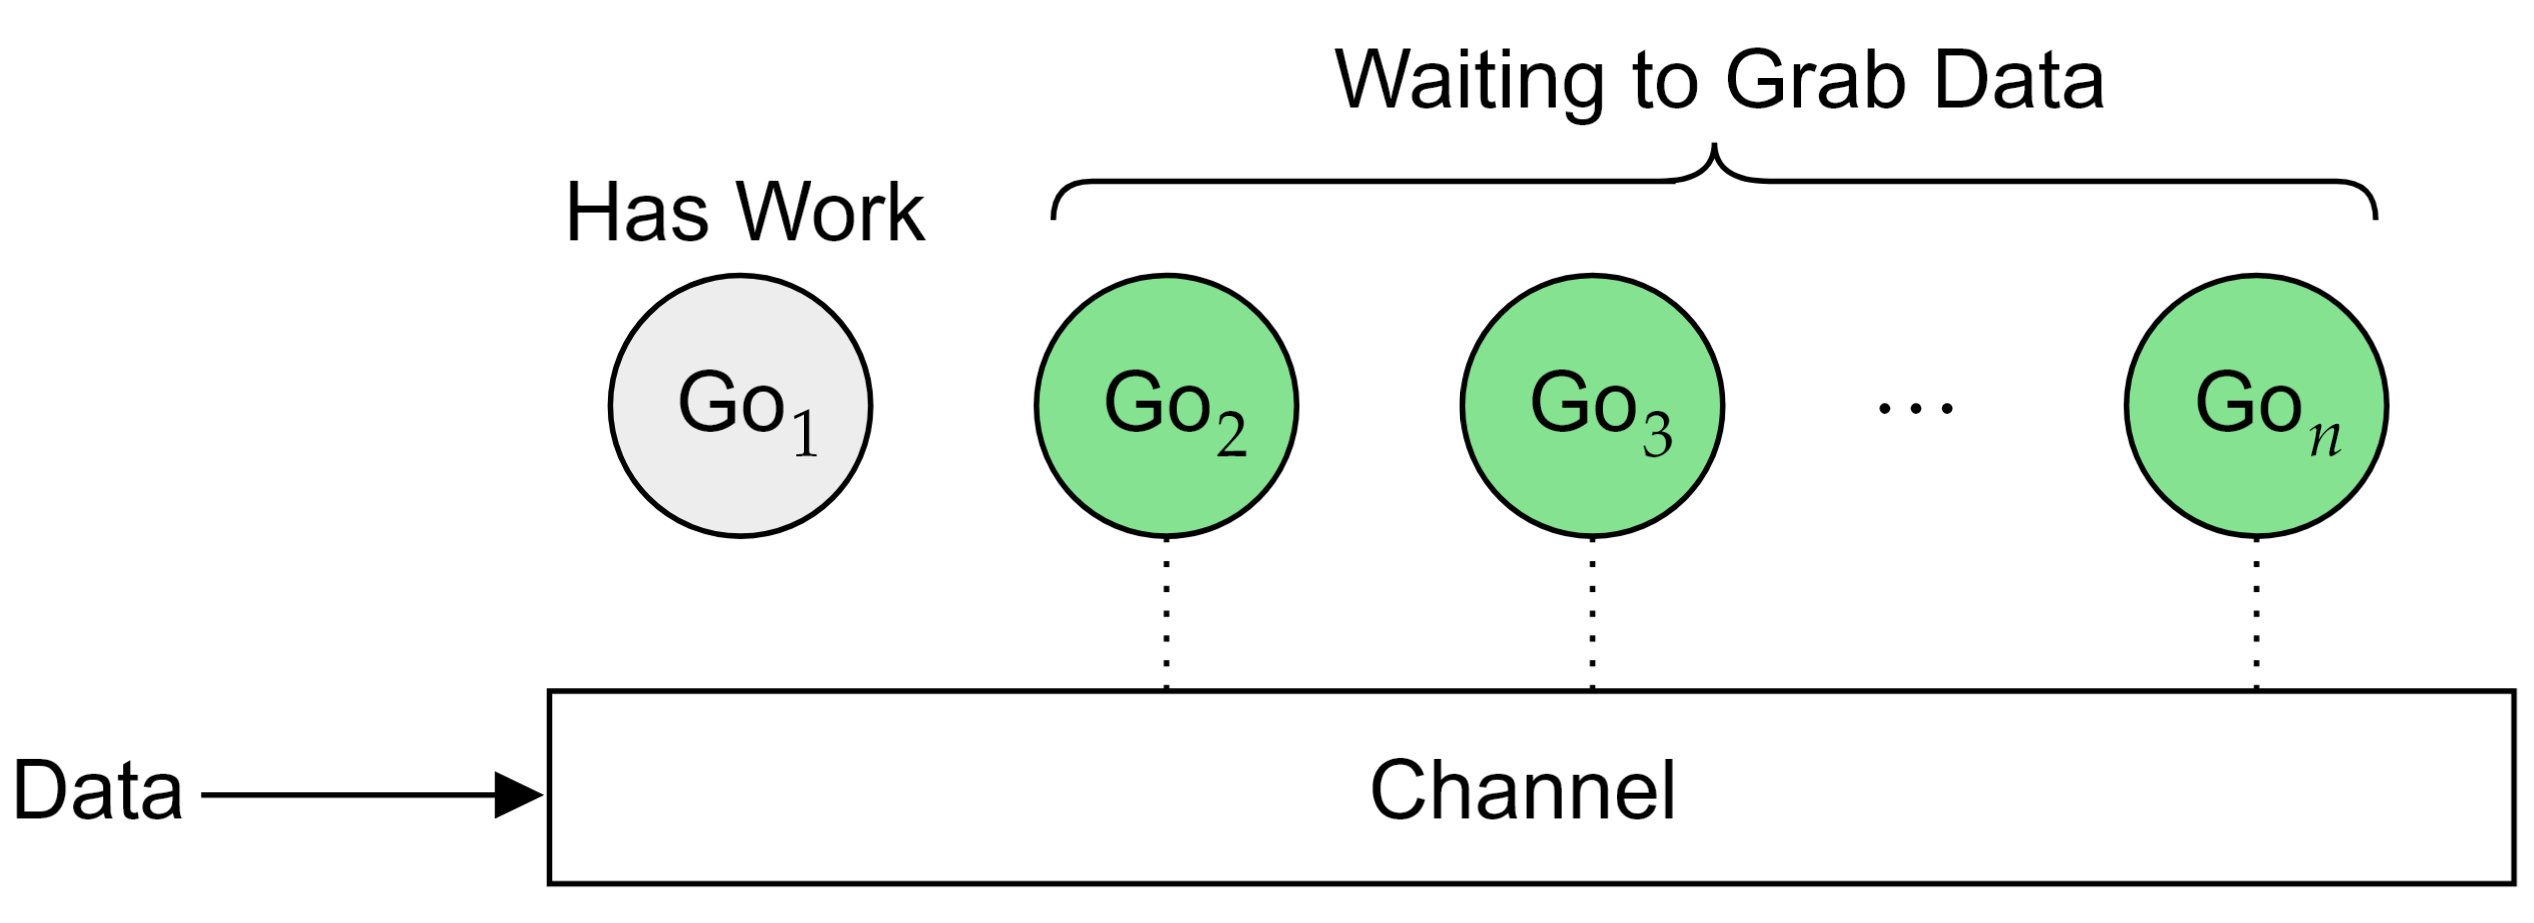
\includegraphics[width=0.8\textwidth]{Sections/rpc/channel.png}
    \caption{A collection of Goroutines competing for the next channel resource.}
    \label{fig:channel}
\end{figure}
\noindent
Note, despite the diagrams order of goroutines, the order in which they run is up to the Go runtime scheduler.

\begin{Example}[Synchronizing Incoming Data Processing]

Consider the following example where we use a channel to synchronize the processing of incoming data:
\begin{lstlisting}[language=Go, caption=Using Channels to Synchronize Downloading and Processing, label={lst:channels}, numbers=none]
    package main

    import (
        "fmt"
        "sync"
        "time"
    )

    // Download function simulates downloading data
    func download(wg *sync.WaitGroup, i int) {
        defer wg.Done()
        fmt.Printf("Downloading: Resource_%d...\n", i)
        time.Sleep(5 * time.Second) // Simulating download time
        fmt.Printf("Download complete: Resource_%d\n", i)
    }

    // Process function simulates processing data
    func process(wg *sync.WaitGroup, i int) {
        defer wg.Done()
        fmt.Printf("Processing: Resource_%d...\n", i)
        time.Sleep(1 * time.Second) // Simulating processing time
        fmt.Printf("Processing complete: Resource_%d\n", i)
    }

    func main() {
        var wg sync.WaitGroup

        // Simulating downloading and processing 5 resources concurrently
        for i := 0; i < 5; i++ {
            wg.Add(1)
            go download(&wg, i)
            wg.Add(1)
            go process(&wg, i)
        }

        wg.Wait()
        fmt.Println("Main function exits")
    }
    \end{lstlisting}
\end{Example}

\newpage 

\begin{theo}[Channel Types]

    In Go, channels can be either \textbf{unbuffered} or \textbf{buffered}:
    \begin{itemize}
        \item \textbf{Unbuffered Channels:} Require a sender and receiver to be ready to communicate. If the receiver is not ready, the sender will block until the receiver is ready.
        \item \textbf{Buffered Channels:} Allow a sender to send data to a channel without the receiver being ready. The channel will store the data until the receiver is ready.
    \end{itemize}
\end{theo}

Unbuffered channels undergo a \textbf{handshake} process:
\begin{figure}[h]
    \centering
    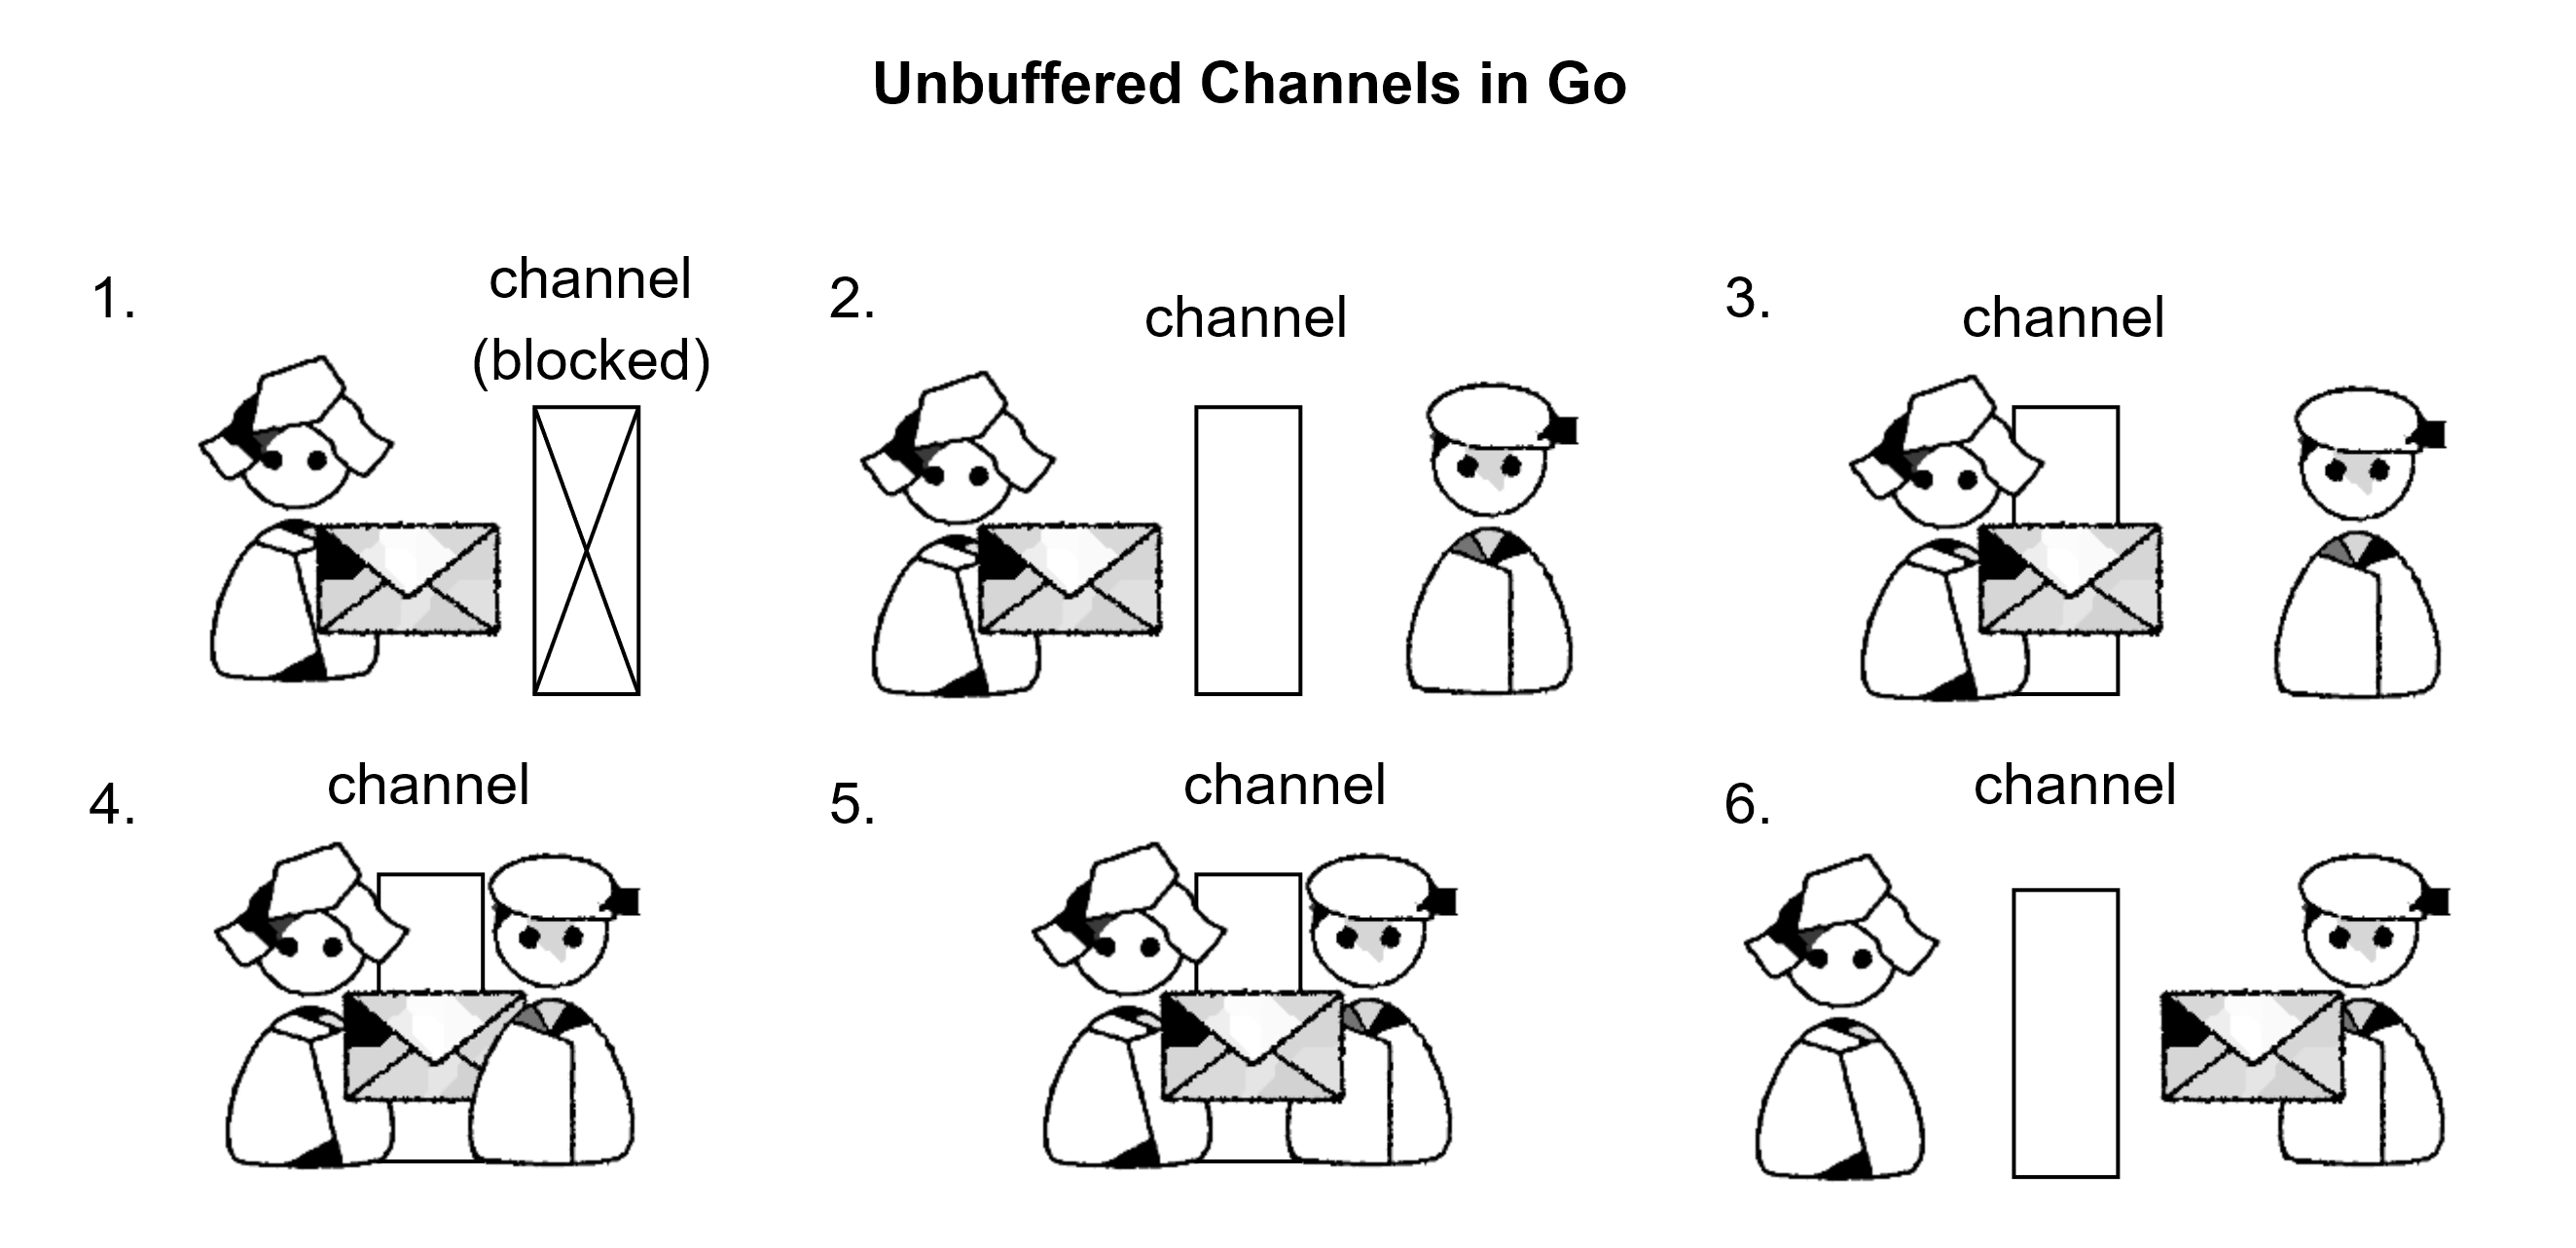
\includegraphics[width=1\textwidth]{Sections/rpc/unbuffered.png}
    \caption{Handshake process of an unbuffered channel.}
    \label{fig:handshake}
\end{figure}

\noindent
Say Alice (left) want to send a message to Bob (right) over a channel. (1) The channel is blocked until Bob is ready to receive. (2) The channel is no longer blocked 
read for the exchange. (3) Alice preforms a \textbf{send} and is locked into the operation until Bob \textbf{receives} the message. (4-5) Bob enters the channel and receives the message;
Both Alice and Bob are locked into the operation until the message exchange is complete.
(6) they both are free to continue their operations.

\newpage 

\noindent
In contrast buffered channels allow for a more asynchronous approach:

\begin{figure}[h]
    \centering
    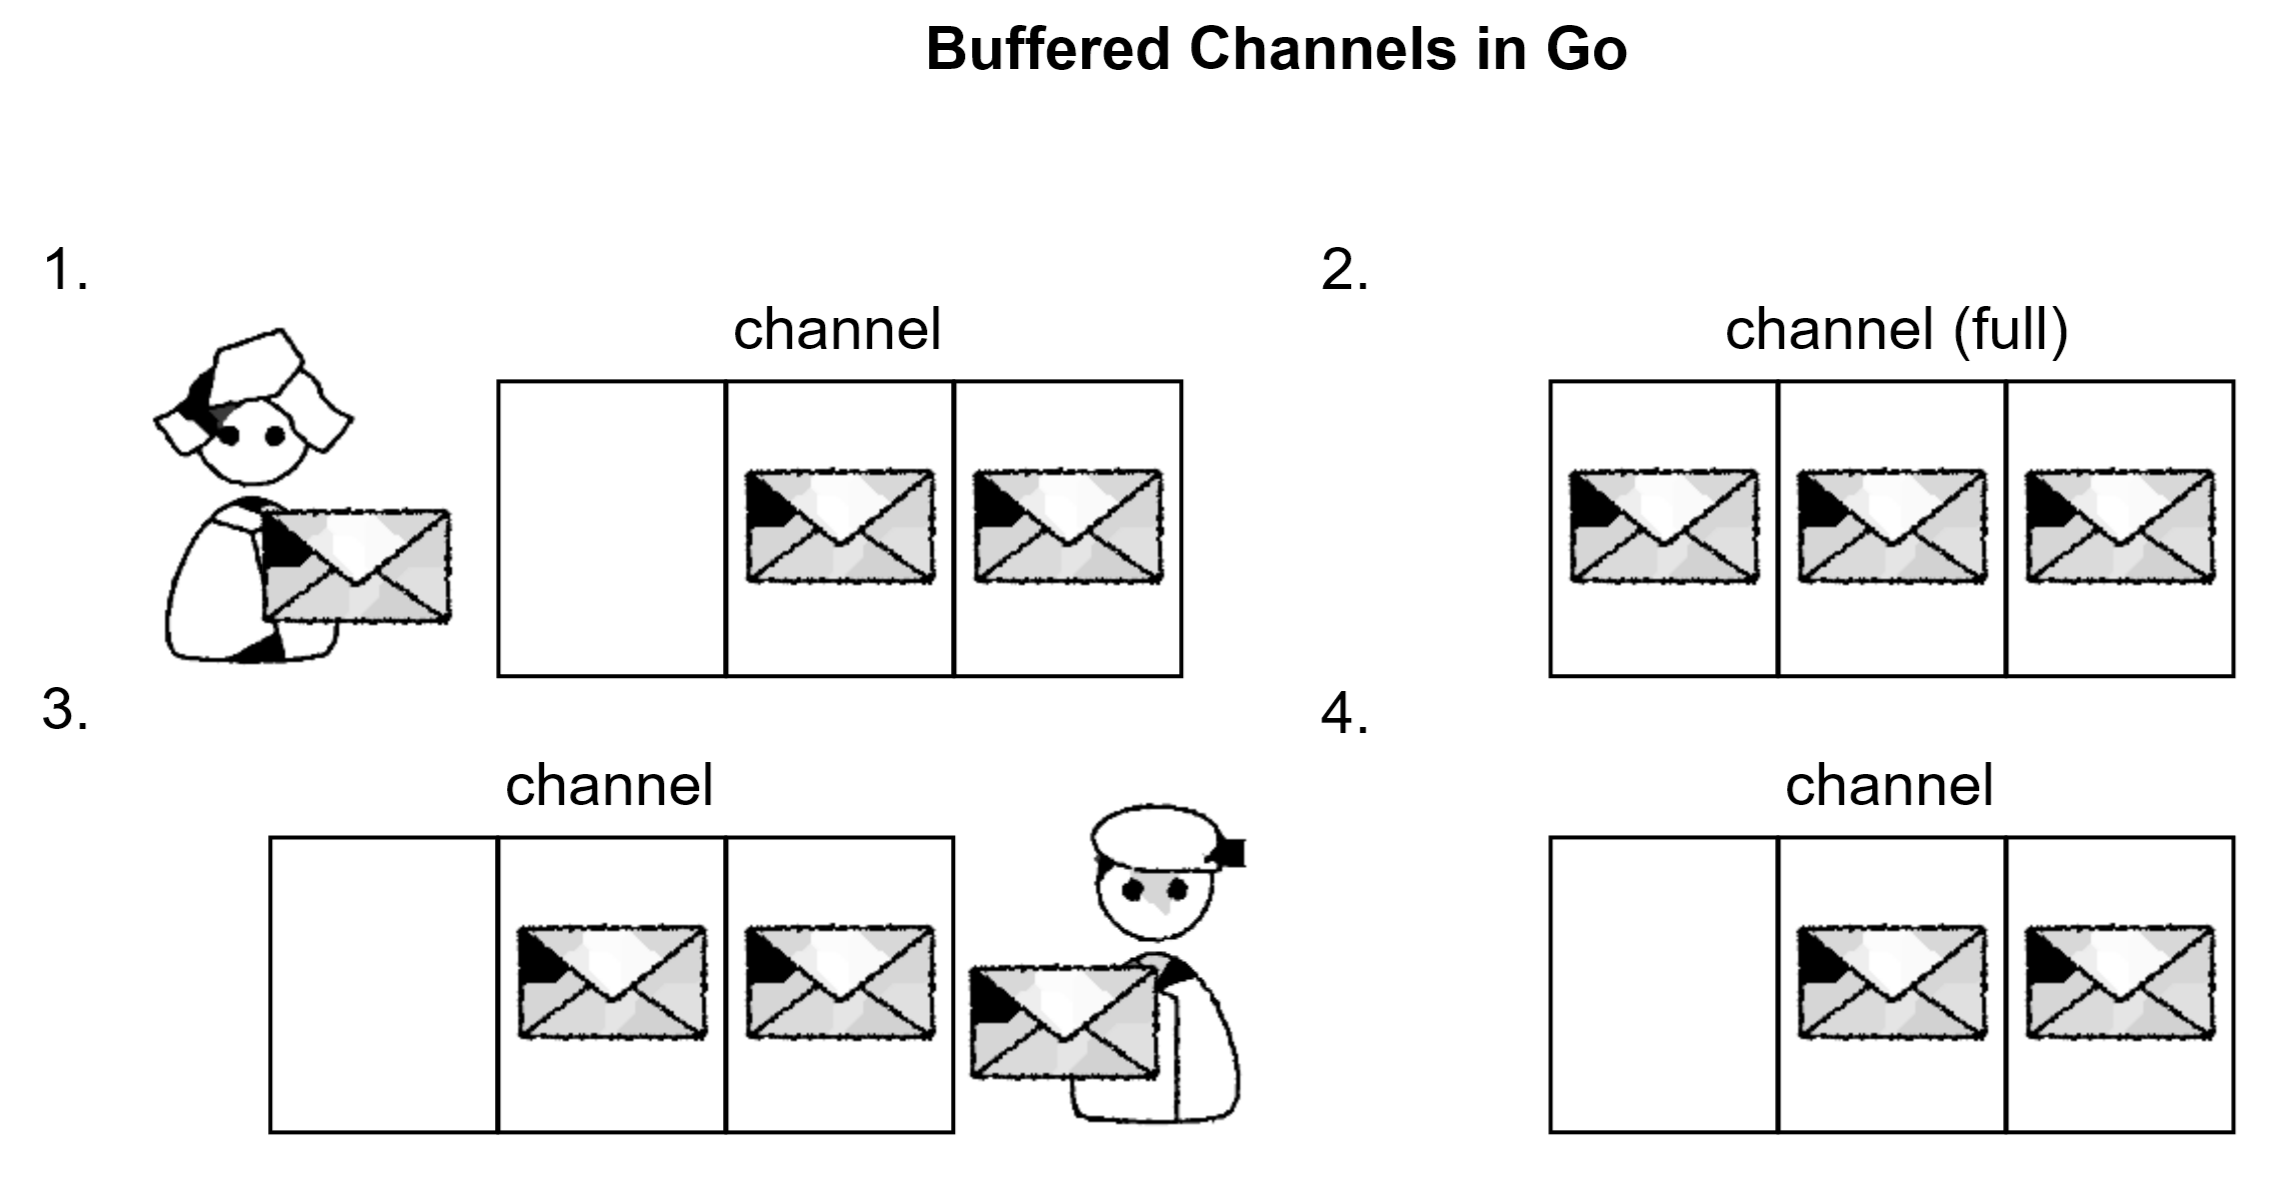
\includegraphics[width=1\textwidth]{Sections/rpc/buffered.png}
    \caption{Buffered channel allowing for asynchronous communication.}
    \label{fig:buffered}
\end{figure}

\noindent
(1) Here Alice (left) fills the channel from left to right with messages. (2) The channel is full and Alice is free to continue her operations. (3) Bob (right) takes the rightmost message from the channel. (4) Bob is free to continue his operations, leaving the channel.

% \newpage 

\subsection{Task, Data, and Pipeline Parallelism}

Task, data, and pipeline parallelism are three common forms of parallelism:

\begin{Def}[Task Parallelism]

    \textbf{Task parallelism} involves running multiple tasks simultaneously. Each task is independent and can run in parallel with other tasks,
    perhaps even on the same data.
\end{Def}
\noindent
In essence, we may think \underline{same data, different tasks}:
\begin{figure}[h]
    \centering
    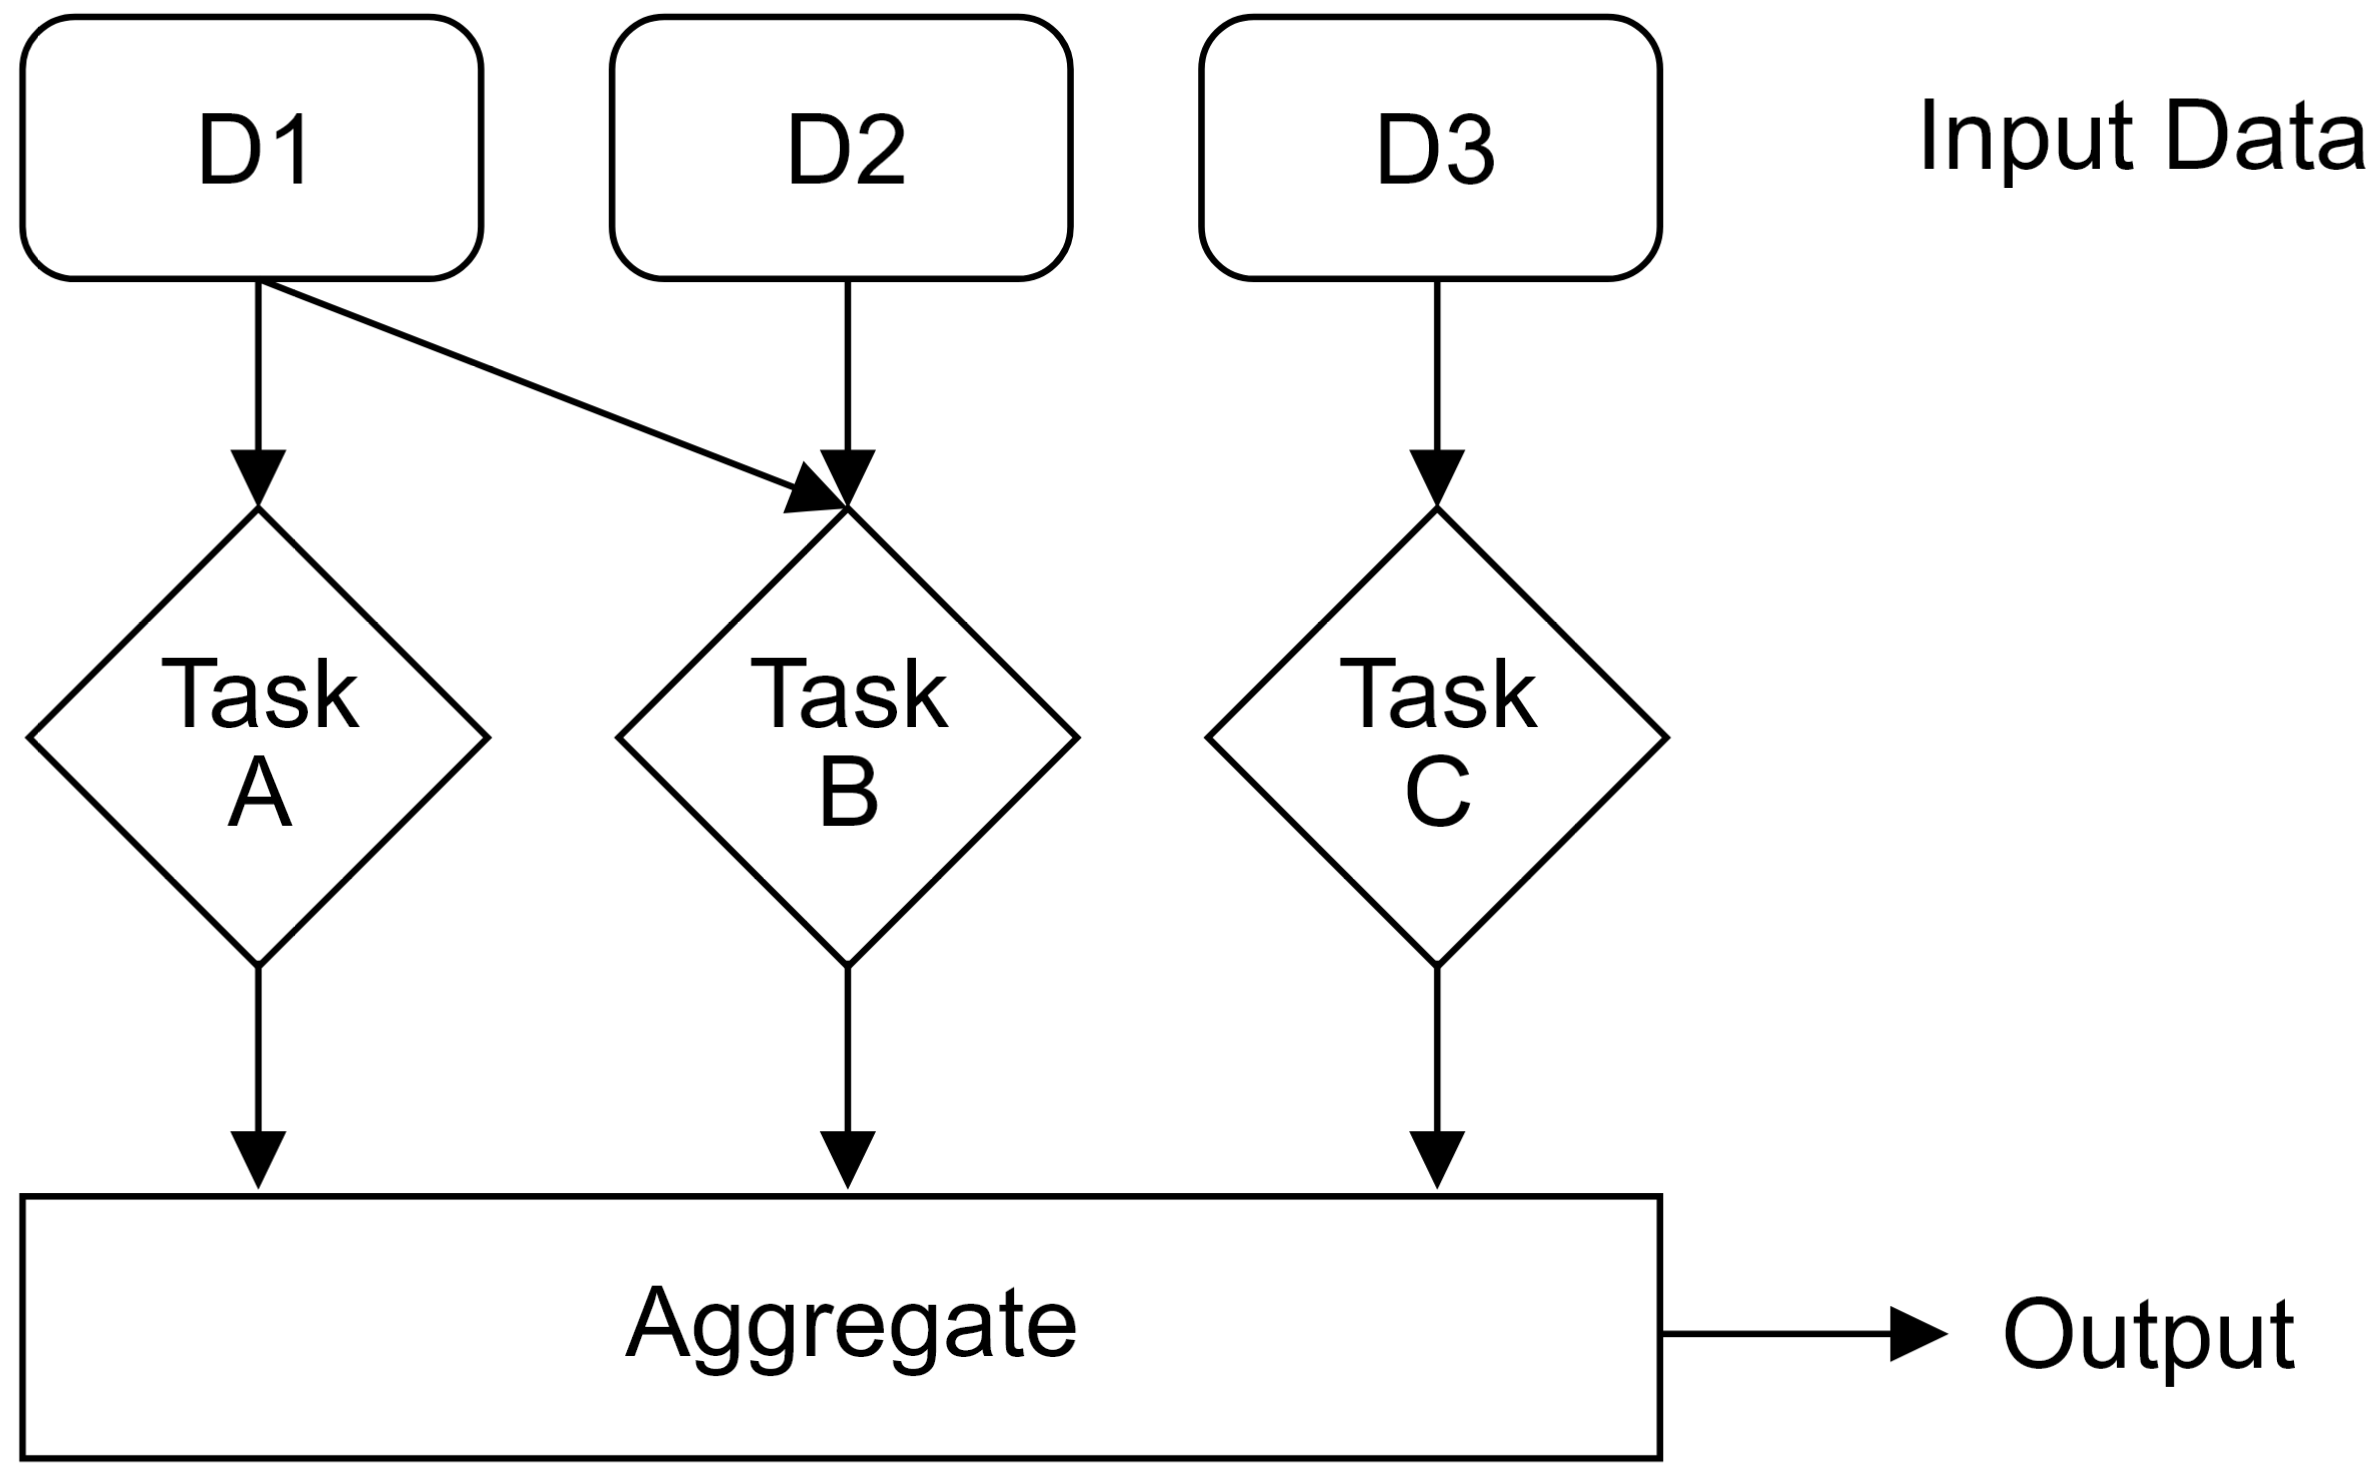
\includegraphics[width=0.5\textwidth]{./Sections/rpc_2/tpar.png}
    \caption{Task Parallelism Culminating into an Aggregate Result}
\end{figure}
\noindent

\vspace{-1em}
\begin{Def}[Data Parallelism]

    \textbf{Data parallelism} involves running the same task on multiple data items. Each task is identical, but the data is different.
\end{Def}
\noindent
We may think \underline{same task, different data}:
\begin{figure}[h]
    \centering
    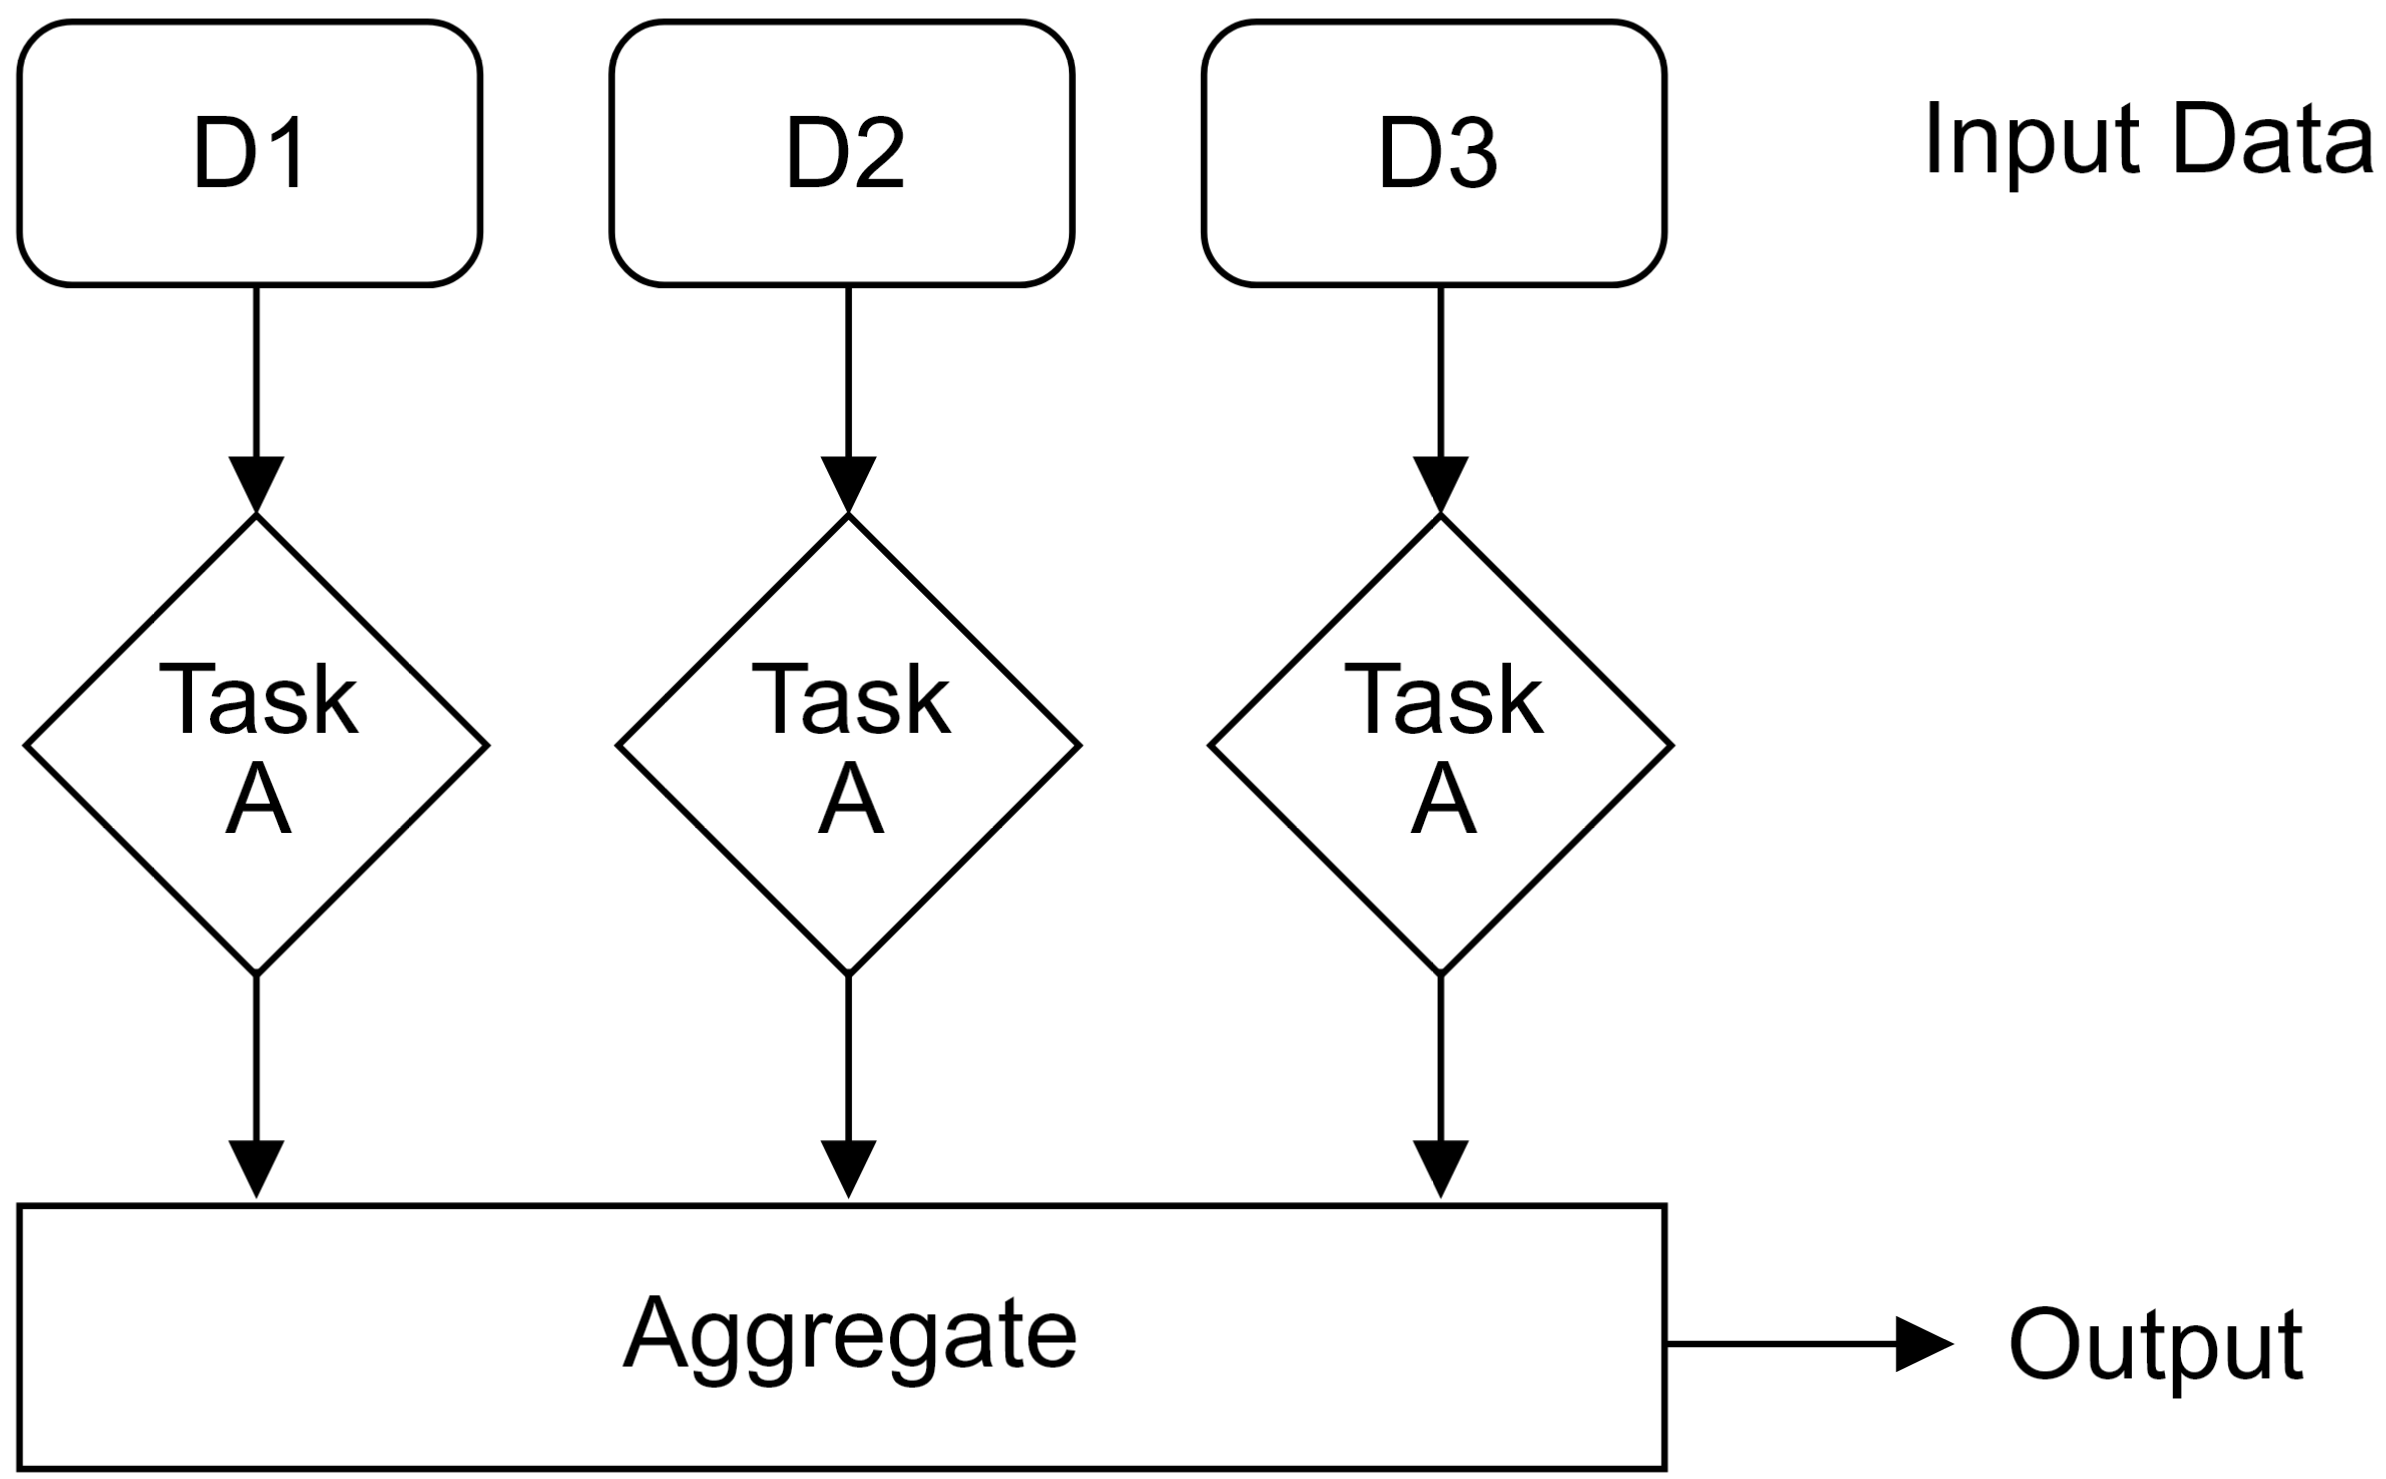
\includegraphics[width=0.5\textwidth]{./Sections/rpc_2/dpar.png}
    \caption{Data Parallelism Culminating into an Aggregate Result}
\end{figure}

\newpage 
\noindent
To continue, we have:
\begin{Def}[Pipeline Parallelism]

    \textbf{Pipeline parallelism} involves breaking a task into multiple stages, each of which can be executed concurrently. The output of one stage is the input to the next stage.
\end{Def}

For instance, consider the following pipeline:
\begin{itemize}
    \item \textbf{Task A}: ``Search for a flight.'' (1 time unit)
    \item \textbf{Task B}: ``Book a flight.'' (1 time unit)
\end{itemize}

\noindent
First consider the scenario where we only have one resource to work with, resulting in concurrency:
\begin{figure}[h]
    \centering
    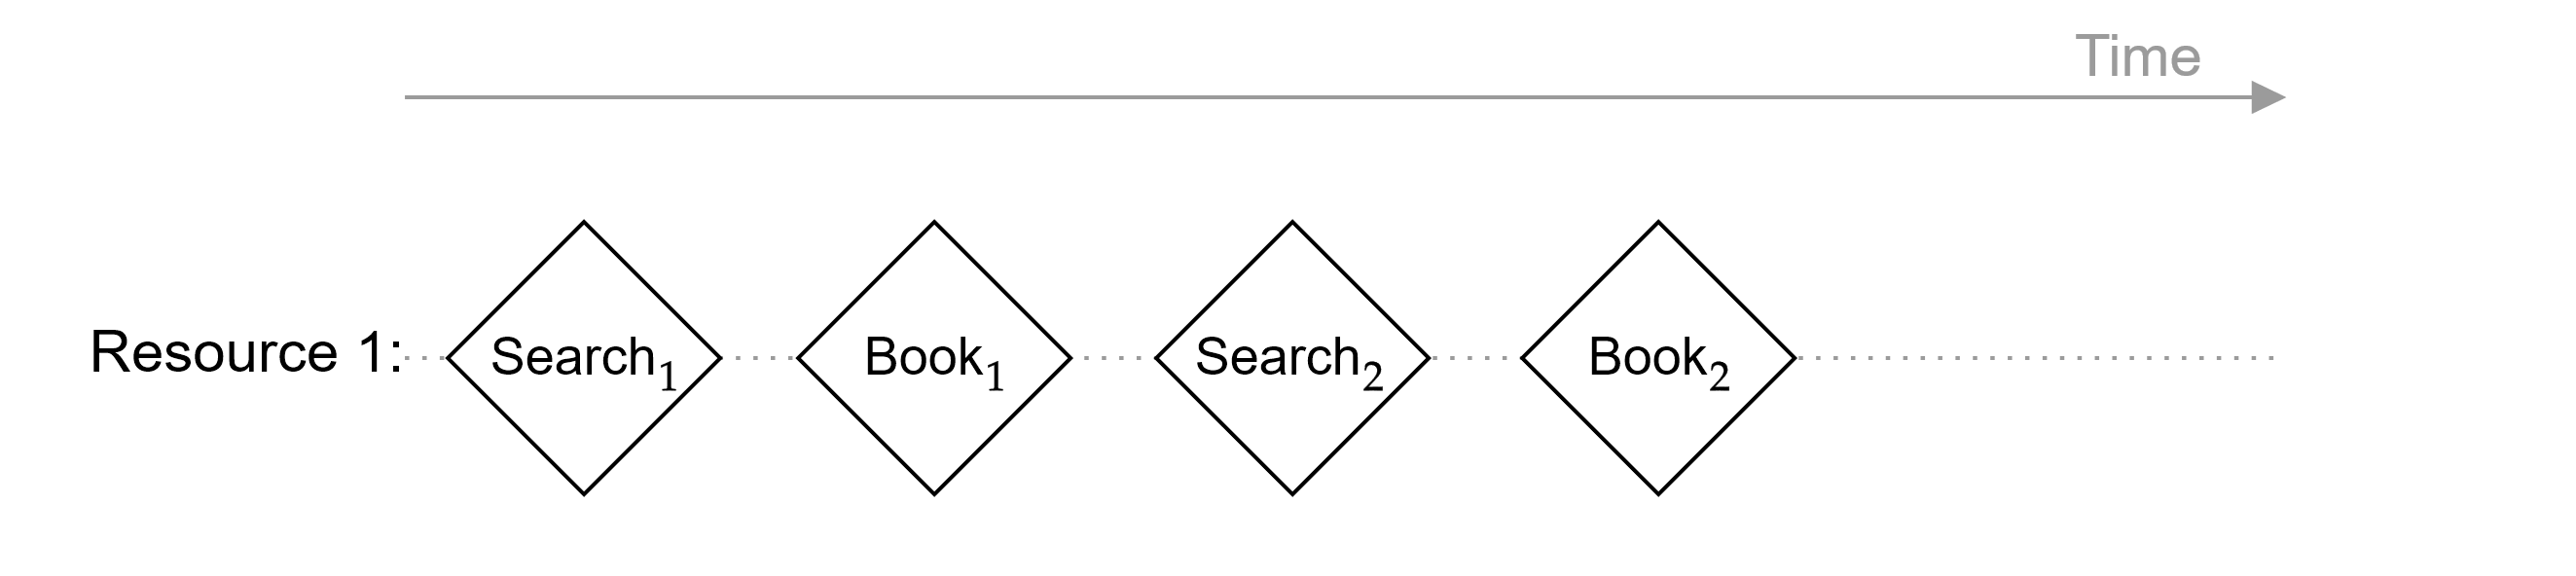
\includegraphics[width=1\textwidth]{./Sections/rpc_2/ppar.png}
    \caption{Searching and Booking flights concurrently}
\end{figure}

\noindent
Now consider the scenario where we have two resources to work with, resulting in parallelism:
\begin{figure}[h]
    \centering
    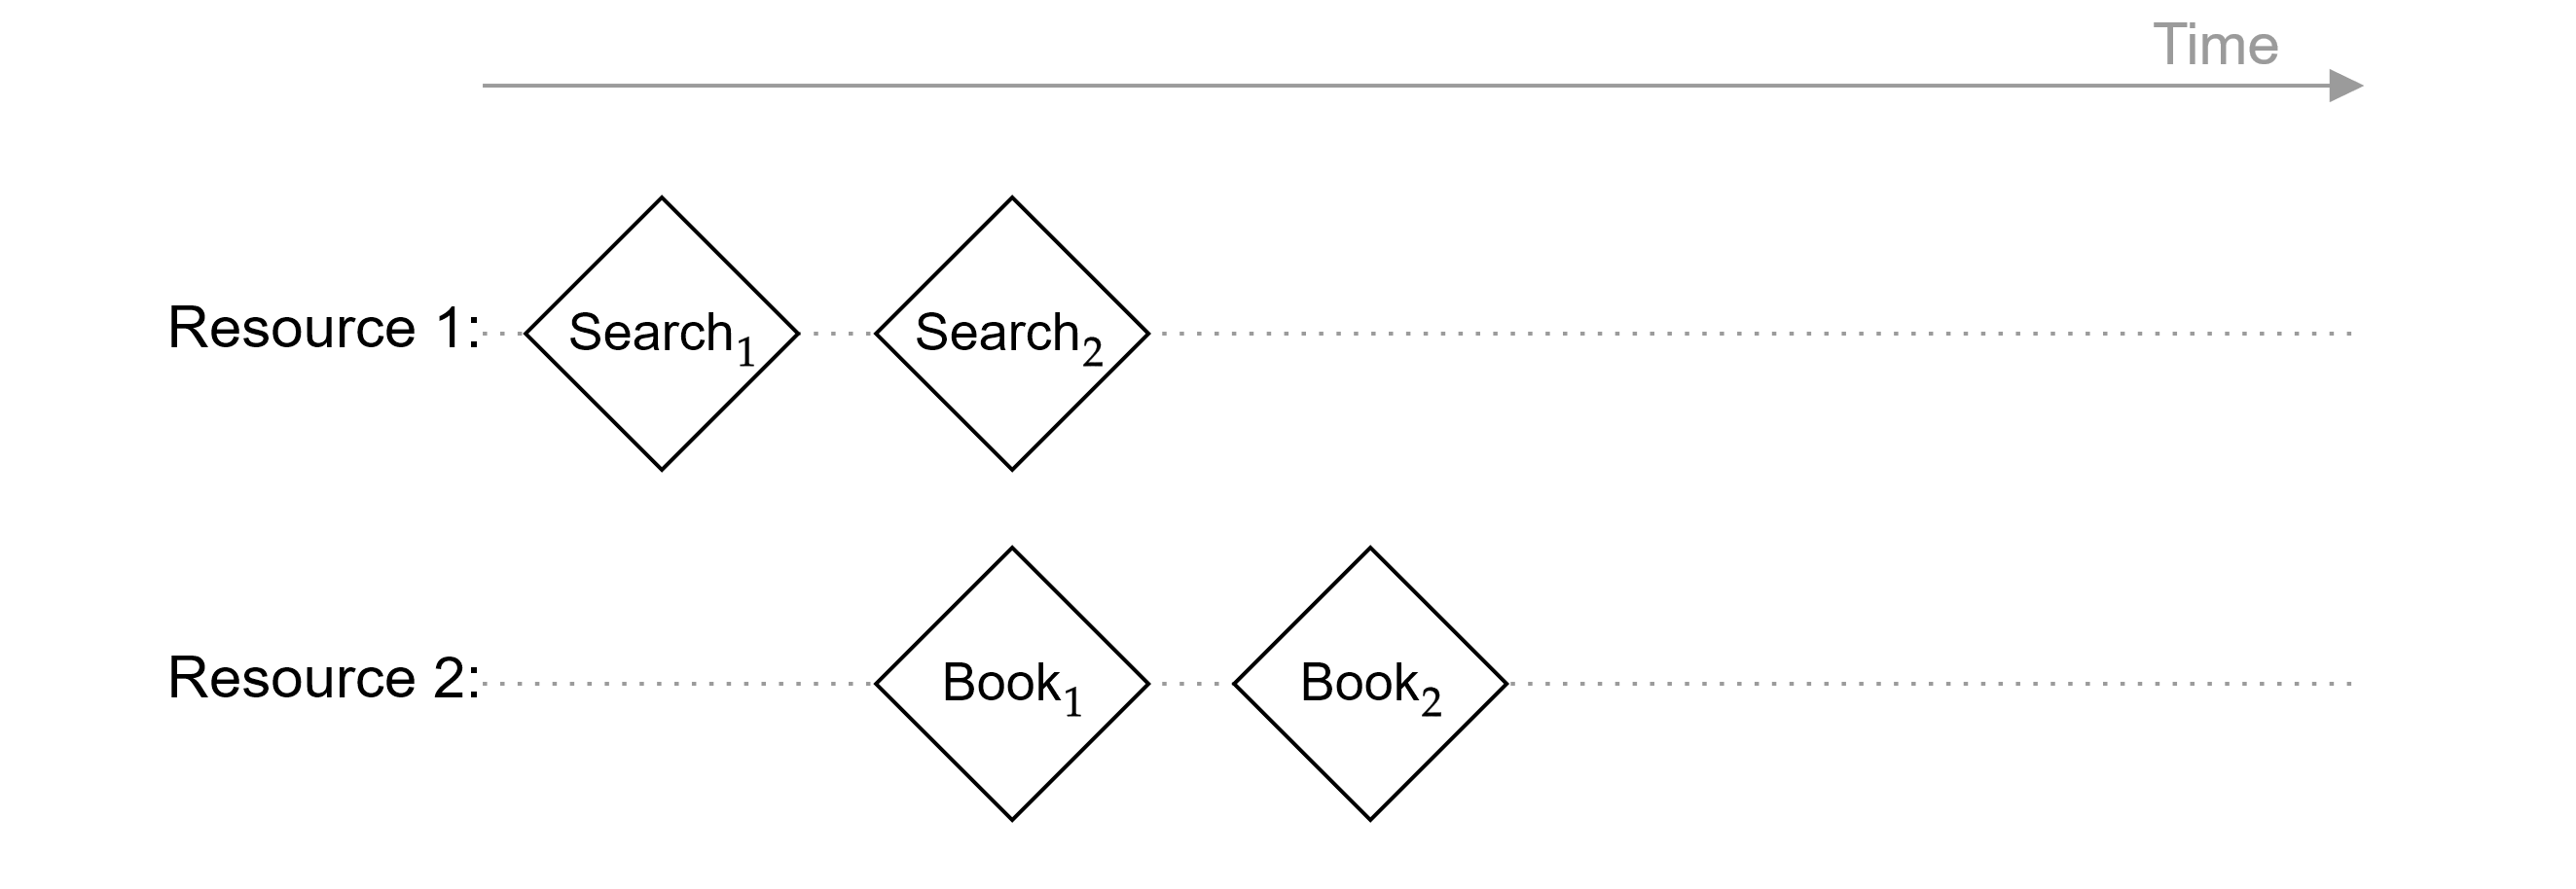
\includegraphics[width=1\textwidth]{./Sections/rpc_2/ppar_2.png}
    \caption{Searching and Booking flights in parallel}
\end{figure}
\noindent
In this case, once the first search is done, we can start booking the flight and search for the next flight in parallel.
\newpage 

\subsection{Arrays \& Slices in Go}

\noindent
Arrays in Go act like arrays in other languages, a fixed-size collection of items of the same type. Slices, on the other hand, allow us to work with a dynamically-sized sequence of elements.

\begin{Def}[Arrays in Go]

    An \textbf{array} in Go is a fixed-size collection of elements of the same data type. Arrays in Go are value types, meaning they are copied when assigned to a new variable.\\
    
    \noindent
    Arrays are declared using the syntax:
    \begin{lstlisting}[language=Go]
    var arr [size]Type
    \end{lstlisting}
    
    \noindent
    For example, an array of integers with 5 elements:
    \begin{lstlisting}[language=Go]
    var numbers [5]int
    \end{lstlisting}
    
    \noindent
    Elements in an array can be accessed using zero-based indexing:
    \begin{lstlisting}[language=Go]
    numbers[0] = 10  // Assign value
    fmt.Println(numbers[0]) // Access value
    \end{lstlisting}
    
    \noindent
    Arrays cannot be resized, and their size must be known at compile time. For dynamic collections, slices are preferred.
\end{Def}

\begin{Example}[Doubling Items in an array]

    Consider the following example where we double each element in an array:
    \begin{lstlisting}[language=Go, numbers=none]
    package main

    import "fmt"

    func main() {
        // Initialize an array
        numbers := [5]int{1, 2, 3, 4, 5}

        // Double each element in the array
        for i := 0; i < len(numbers); i++ {
            numbers[i] *= 2 // Shorthand for numbers[i] = numbers[i] * 2
        }

        // Print the modified array
        fmt.Println(numbers)
    }
    // Output: [2 4 6 8 10]
    \end{lstlisting}
\end{Example}

\newpage
    
\noindent
In contrast, slices:

\begin{Def}[Slices in Go]
    
    A \textbf{slice} is a dynamically-sized reference to a portion of a single underlying array.

    \noindent
    Slices are declared using square brackets without specifying a fixed size:
    \begin{lstlisting}[language=Go]
    var numbers []int // A slice of integers
    \end{lstlisting}
    
    \noindent
    Slices are typically created using the \snippet{make} function or by slicing an existing array:
    \begin{lstlisting}[language=Go]
    // Using make()
    numbers := make([]int, 5) // Creates a slice with length 5
    
    // Slicing an array
    arr := [5]int{1, 2, 3, 4, 5}
    slice := arr[1:4] // Slice from index 1 to 3 -> {2, 3, 4}
    \end{lstlisting}
    
    \noindent
    Slices maintain a reference to the original array, meaning modifications affect both:
    \begin{lstlisting}[language=Go]
    arr := [5]int{1, 2, 3, 4, 5}
    slice := arr[1:3]
    slice[0] = 99 // Modifies arr[1] as well
    fmt.Println(arr)  // Output: [1 99 3 4 5]
    \end{lstlisting}

    \noindent
    The \snippet{append()} function modifies slices given there's enough capacity:
    \begin{lstlisting}[language=Go]
    arr := [5]int{1, 2, 3, 4, 5}
    slice := arr[:1] // Slice from index 0 to 0 -> {1}
    slice = append(slice, 7, 8) // Adds elements to the slice
    fmt.Println(slice) // Output: [1 7 8]
    fmt.Println(arr)   // Output: [1 7 8 4 5] (modified)
    \end{lstlisting}

    \noindent
    If \snippet{append()} exceeds the slice's capacity, a new array is allocated and referenced by the slice:
    \begin{lstlisting}[language=Go]
    ... // Previous code
    fmt.Println(cap(slice)) // Output: 5 (capacity of the slice)
    slice = append(slice, 7, 8, 9, 10, 11) // Exceeds capacity, (6 total)
    fmt.Println(slice) // Output: [1 7 8 9 10 11]
    fmt.Println(arr)   // Output: [1 2 3 4 5] (unchanged)
    \end{lstlisting}

    \noindent
    To copy an array to a slice, use the \snippet{copy()} function:
    \begin{lstlisting}[language=Go]
    arr := [5]int{1, 2, 3, 4, 5}
    slice := make([]int, len(arr))
    copy(slice, arr) // Syntax: copy(destination, source)
    slice[0] = 99
    fmt.Println(slice) // Output: [99 2 3 4 5]
    fmt.Println(arr)   // Output: [1 2 3 4 5] (unchanged)
    \end{lstlisting}
\end{Def}

\newpage 
\subsection{Repeating Tasks: Tick and Ticker in Go}

In Go, the \snippet{time} package provides two types for repeating tasks at regular intervals:

\begin{Def}[\texttt{time.Tick} and \texttt{time.Ticker} in Go]

    The \texttt{time} package in Go provides two mechanisms for scheduling repeated tasks at fixed intervals:
    
    \begin{itemize}
        \item \textbf{\snippet{time.Tick(duration)}}: Returns a channel that sends the current time at regular intervals. It is a convenience function but \textbf{}{cannot be stopped}.
        \item \textbf{\snippet{time.NewTicker(duration)}}: Creates a \snippet{Ticker} object, which provides a \snippet{.Stop()} method to halt the ticker. Additionally the \snippet{.C} returns a channel from which the signal can be read.
    \end{itemize}
\end{Def}

\begin{Example}[Record a signal n times every second]

    Say we want to record a signal $n$ times every second. We can use a \snippet{time.Ticker}:
    \begin{lstlisting}[language=Go, numbers=none]
    package main
    import "fmt"; import "time"; import "sync"
    
    func Status(ch <-chan time.Time, wg *sync.WaitGroup) {
        defer wg.Done()
        <-ch // Wait for signal
        fmt.Println("Status: OK")
    }
    
    func main() {
    
        n := 5
        ticker := time.NewTicker(time.Second)
        tickerChan := ticker.C
        var wg sync.WaitGroup
    
        // Spawns n goroutines which waiting for the signal
        for i := 0; i < n; i++ {
            wg.Add(1)
            go Status(tickerChan, &wg)
        }
        wg.Wait()
        ticker.Stop()
    }
    \end{lstlisting}

    \noindent
    This type of example can be extended to perform any task at a given interval.
\end{Example}
    
% \newpage

\section{Time, Clocks, and Logical Ordering}
\subsection{Accuracy of Time: Atomic Clocks \& NTP}
\noindent
Time allows us to order and identify events. 
Say we ran \snippet{time.Now()} on two different machines:

\begin{figure}[h]
    \centering
    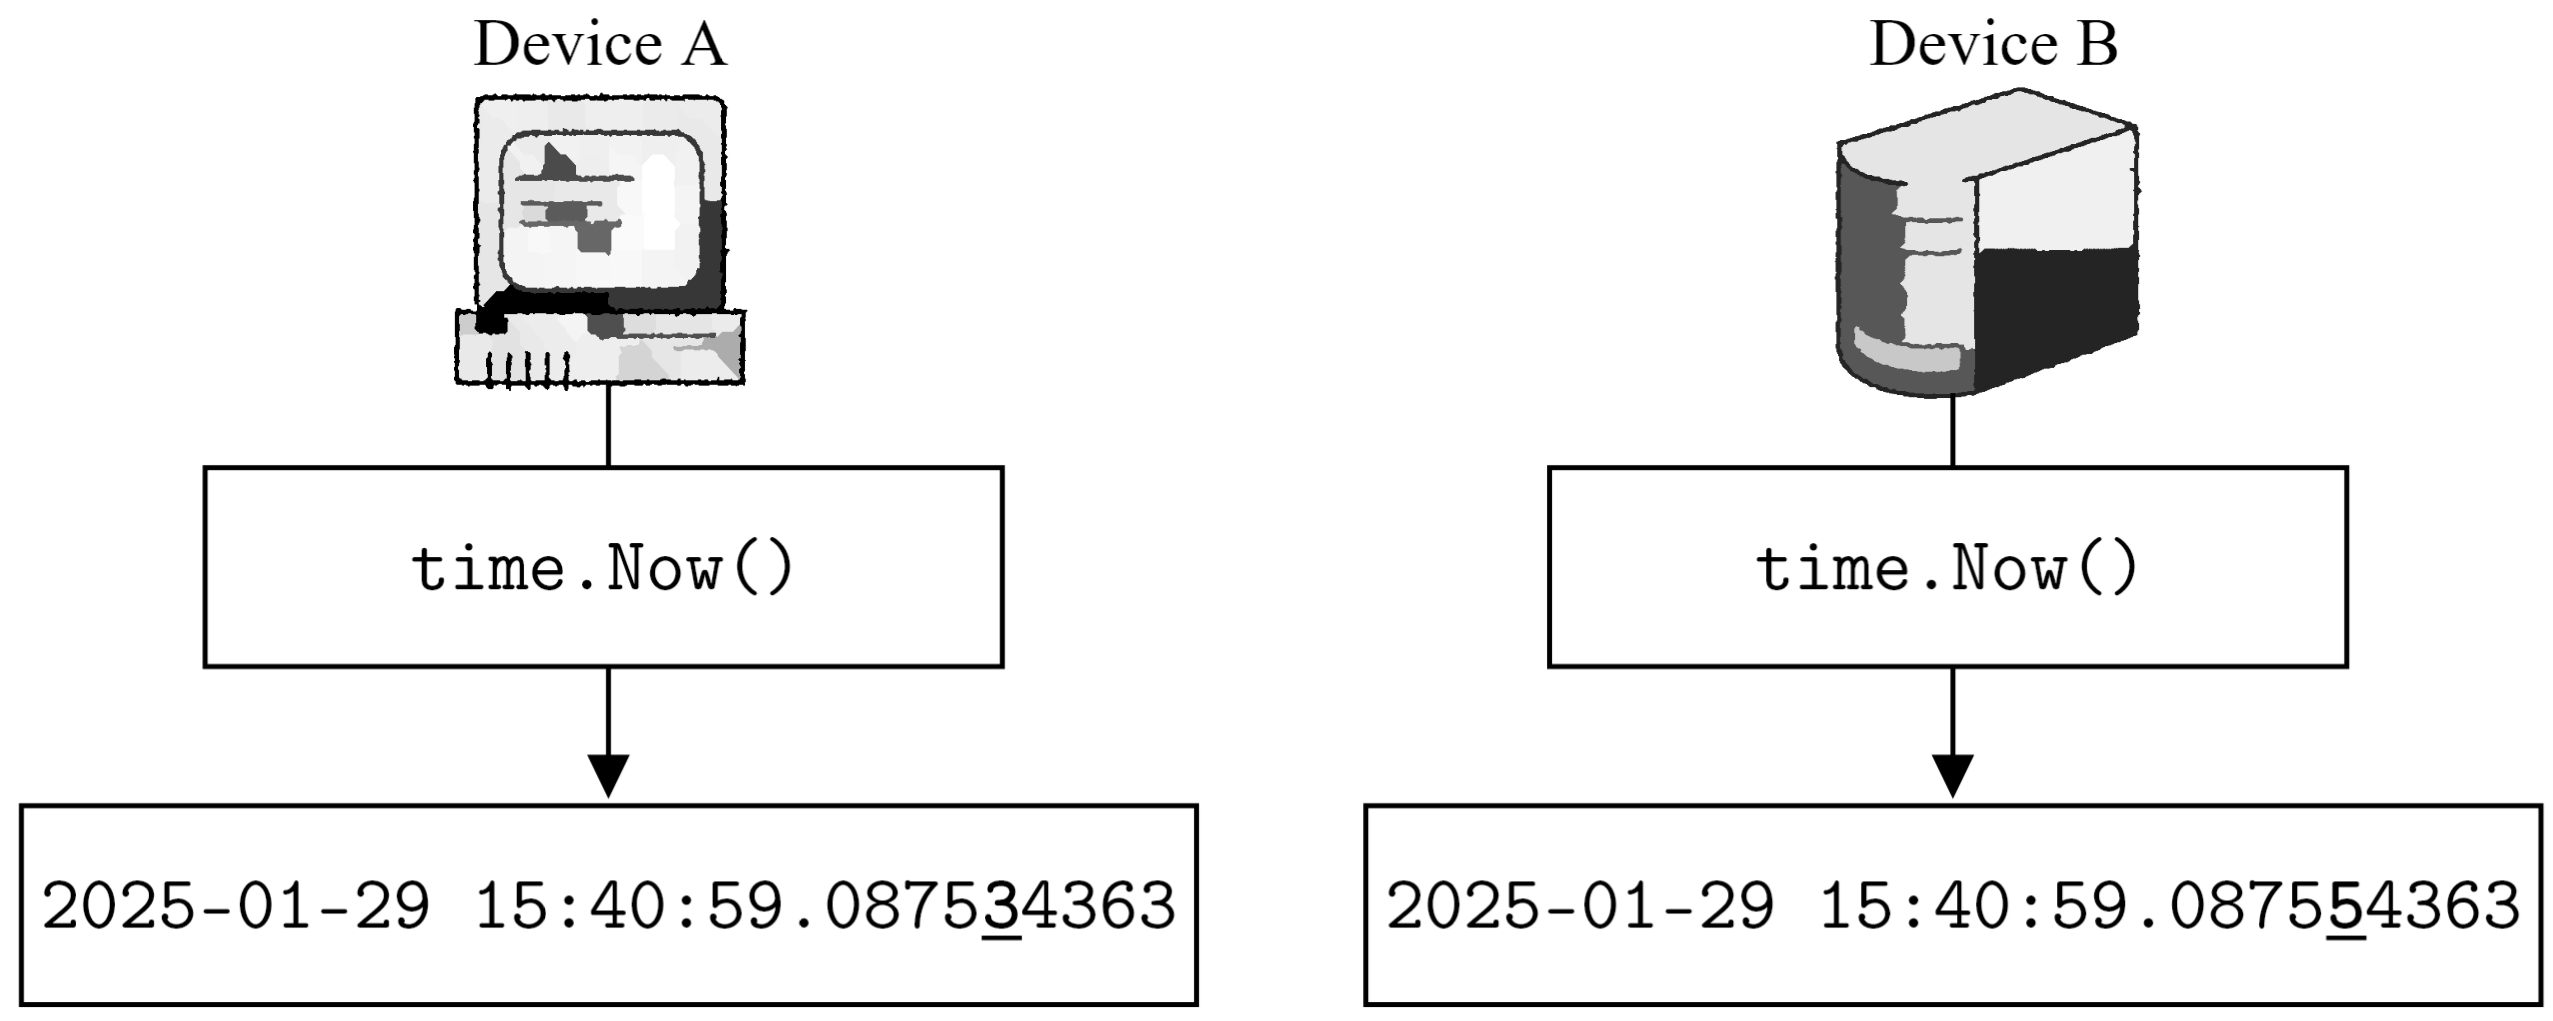
\includegraphics[width=.9\textwidth]{./Sections/time/now.png}
    \caption{Using \snippet{time.Now()} on two different machines}
\end{figure}

\noindent
Despite Device $A$ appearing to be ahead of Device $B$, we cannot be certain via 
the following reasons:

\begin{theo}[Clock Synchronization Impossibility]

    There are two key reasons why perfect clock synchronization is impossible:

    \begin{itemize}
        \item \textbf{Clock Skew:} There's a difference between every system clock (ideally 0), as they maintain their own local clock via a hardware oscillator incrementing a counter register.
        \item \textbf{Clock Drift:} Even if systems initialize with a reference time, their clocks will inevitably diverge due to variations in manufacturing, age, or environmental factors such as temperature.
        We measure the deviation by, $\dfrac{dC}{dt}=1+\rho$, where $C$ is the clock time and $t$ is the real time, and $\rho$ (rho) is the drift rate (ideally 0).
    \end{itemize}
\end{theo}

\noindent
We may formalize what we may consider synchronized clocks as follows:
\begin{Def}[Clock Synchronization Threshold]
    
    Let there be two clocks $C_i$ and $C_j$. They are (delta) $\delta$-synchronized if for all $t$ time units:
    \[ |C_i(t) - C_j(t)| \leq \delta \]

    \noindent
    \textbf{E.g.,} $C_i$ and $C_j$ are $\delta$-synchronized within 10ms if $|C_i(t) - C_j(t)| \leq 10ms$
\end{Def}

\newpage 

\noindent
In practice we to achieve semi-synchronized clocks, we developed the following protocol:

\begin{Def}[Network Time Protocol (NTP)]
    
    The NTP is a protocol synchronizes network clocks via a ground-truth time distribution system.
    The ground-truth time is are GPS satellite \textbf{atomic clocks}, which exhibit negligible drift over millions of years.

    NTP employs a \textbf{round-trip time (RTT)} calculation to estimate the clock offset request latency. 
    It also organizes synchronization strength into a \textbf{stratum hierarchy}, where lower-numbered stratums indicate more accurate time sources:

    \begin{itemize}
        \item \textbf{Stratum 0:} Ground truth \textbf{atomic clocks}/\textbf{GPS receivers}.
        \item \textbf{Stratum 1:} NTP servers that directly synchronize with Stratum 0 reference clocks.
        \item \textbf{Stratum 2:} NTP servers synchronized to Stratum 1 servers.
        \item \textbf{Stratum 3 and beyond:} Weaker NTP servers synchronized to higher-stratum servers.
        \item \textbf{Stratum 16:} A system considered \textit{unsynchronized} (e.g., a freshly booted system).
    \end{itemize}
\end{Def}

\vspace{-1em}
\begin{figure}[h]
    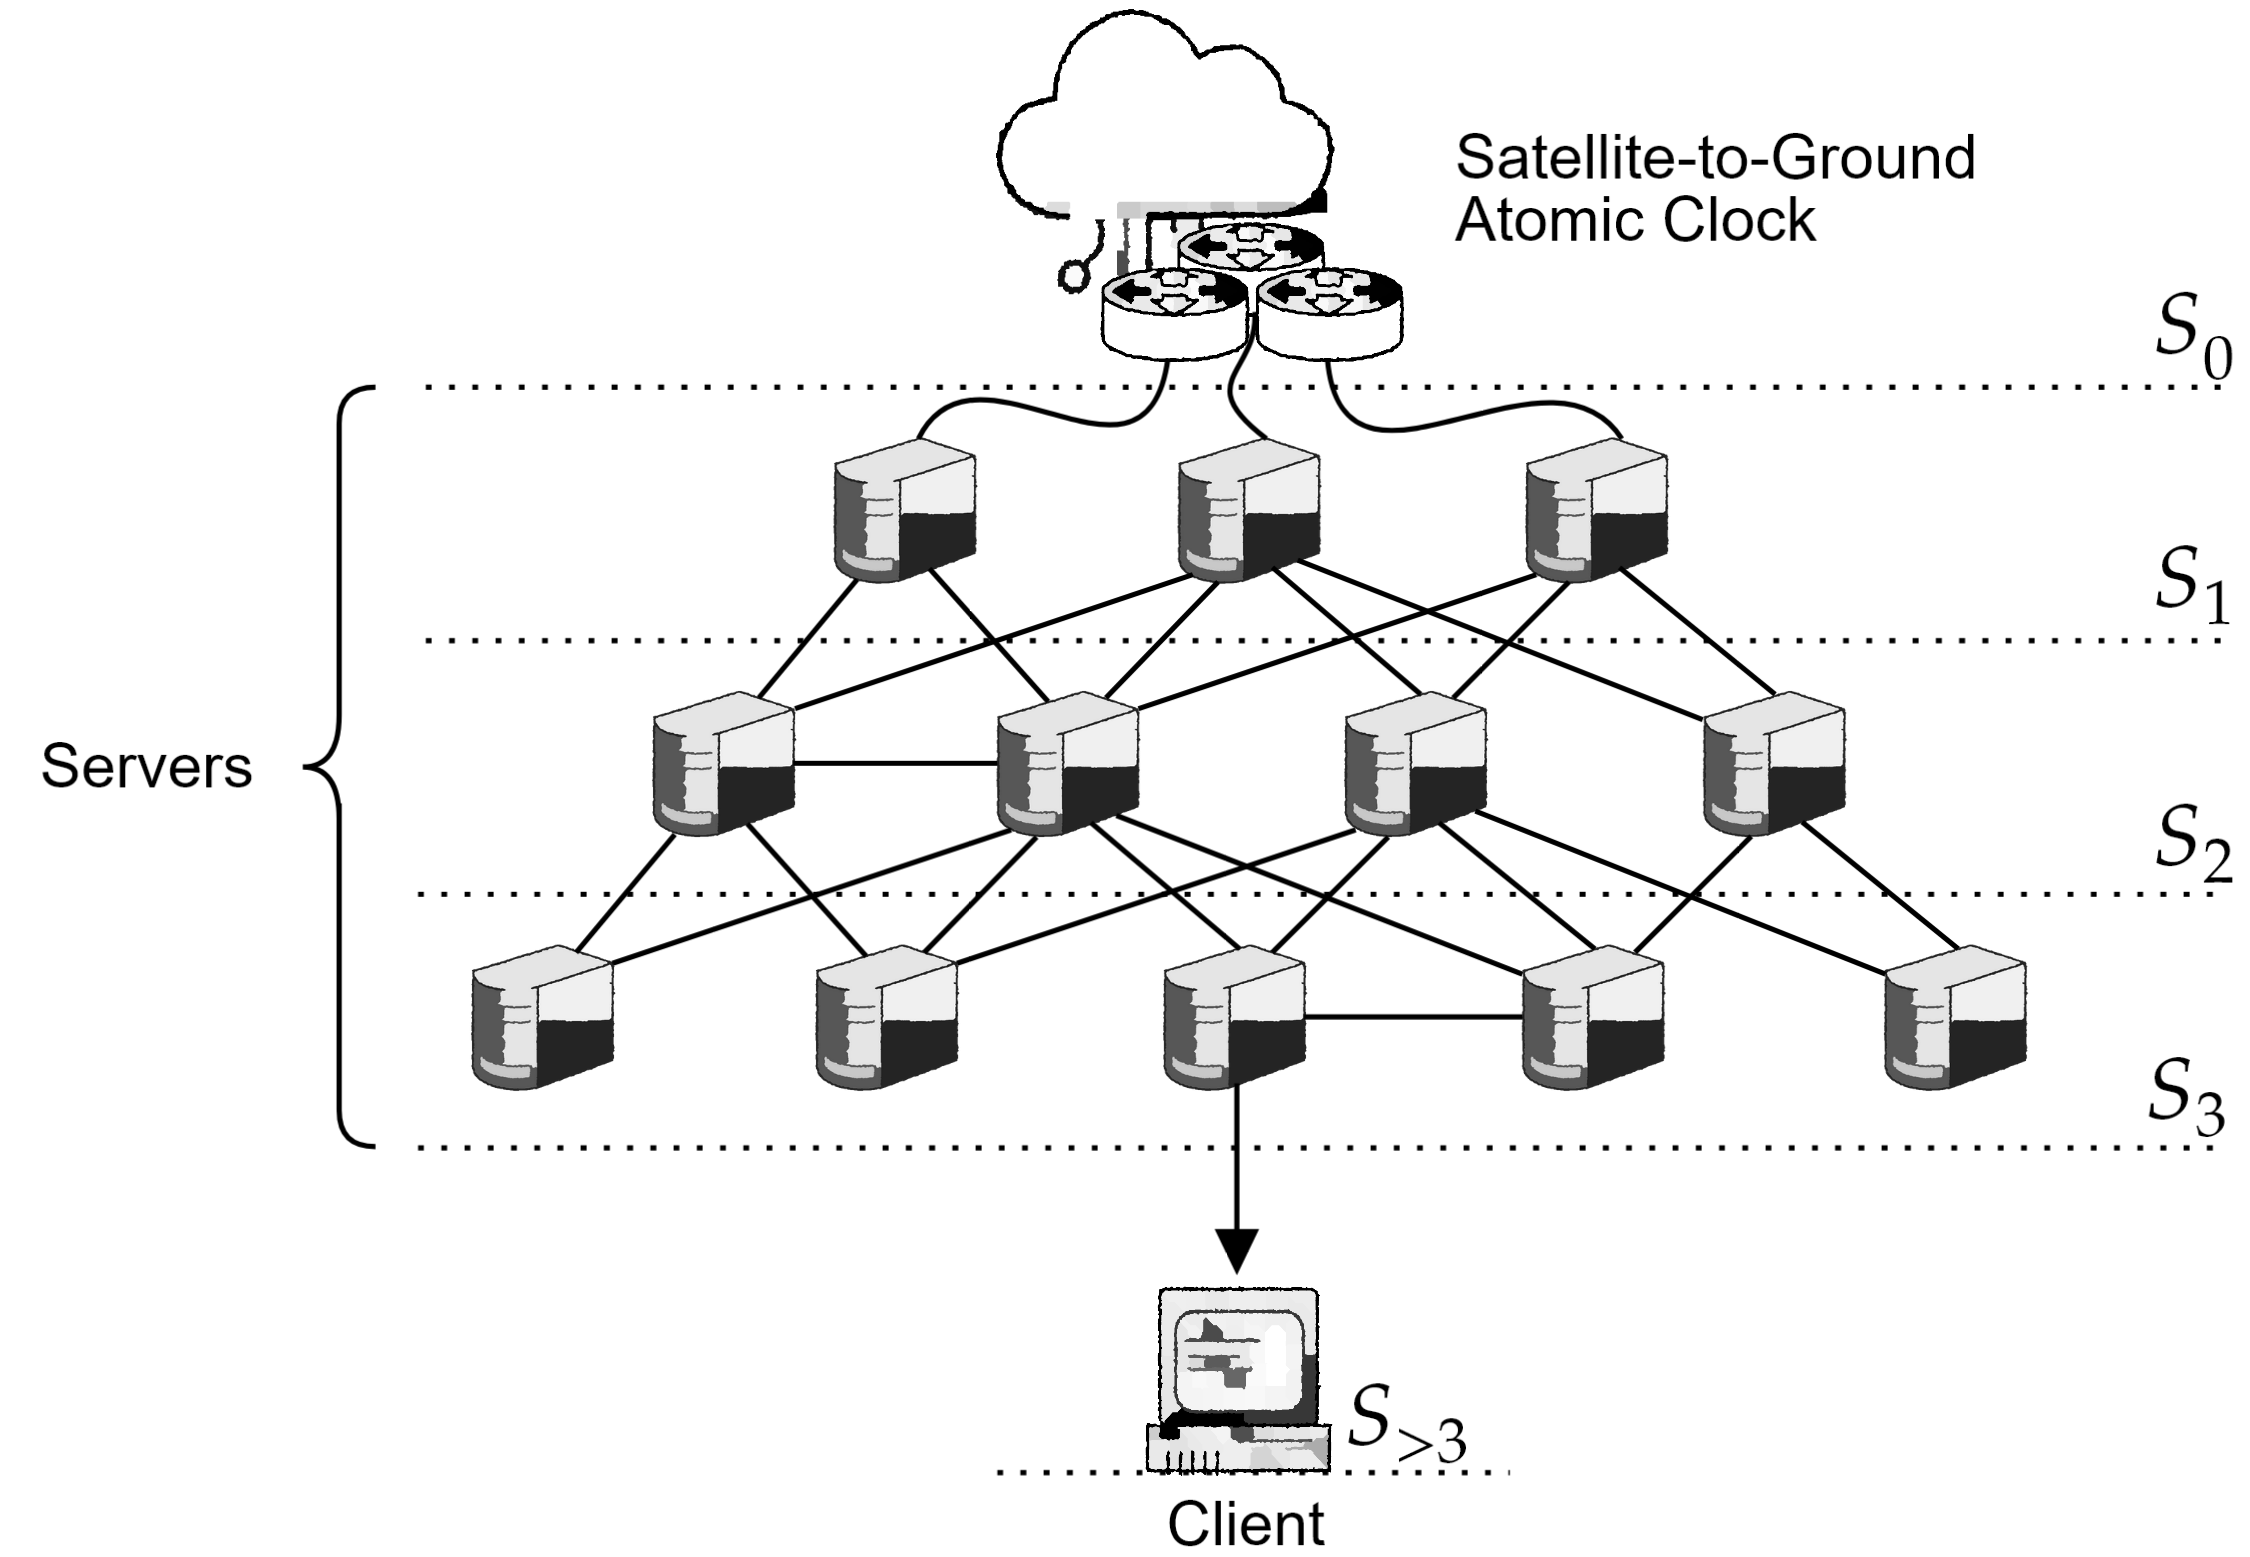
\includegraphics[width=.9\textwidth]{./Sections/time/sat.png}
    \caption{NTP Stratum Hierarchy From GPS Satellite Atomic Clock to Client.}
\end{figure}

\newpage 
\subsection{Logical Clocks: Lamport \& Vector Clocks}

\noindent
To get away from the limitations of physical clocks, we may use logical clocks to order events.

\begin{Def}[Logical Clocks]

    Let $a$ and $b$ be two events part of a totally ordered set of events. Let function $t(x)$ denote the time of event $x$. Then,
    \[ a \rightarrow b \implies t(a) < t(b) \]

    \noindent
    Where $a \rightarrow b$ denotes that event $a$ happens before $b$, which implies $t(a) < t(b)$.
\end{Def}

\noindent
We may become more formal about cause and effect relationships with the following definition:
\begin{Def}[Causal Order]

    For $r$ \textbf{execution trace} (sequence of events), the causal order relationship $\rightarrow_r$ is defined as:

    \begin{itemize}
        \item If $a$ \textbf{happens before} $b$ in the same process, then $a \rightarrow_r b$.
        \item If $a$ is a \textbf{sender} and $b$ the \textbf{receiver}, then $a \rightarrow_r b$.
        \item \textbf{Transitive Property}: if $a \rightarrow_r b$ and $b \rightarrow_r c$, then $a \rightarrow_r c$.
        \item Events $a$ and $b$ are \textbf{concurrent} (denoted as $a \parallel b$) if:
            \begin{itemize}
                \item[$\blacktriangleright$] $a \not\rightarrow_r b$ and $b \not\rightarrow_r a$, meaning neither event happened before the other.
            \end{itemize}
    \end{itemize}
\end{Def}
\begin{Example}[Causal Order Example]

    \label{ex:causal}
    Determine the causal order relationship between events in processes $P$ and $P'$:

    \begin{itemize}
        \item (a): $a\ ?\ b;\quad $ (b): $a\ ?\ k;\quad$ (c): $ c\ ?\ b;\quad$ (d): $ c\ ?\ e$
    \end{itemize}

    

    \hspace{4em}
    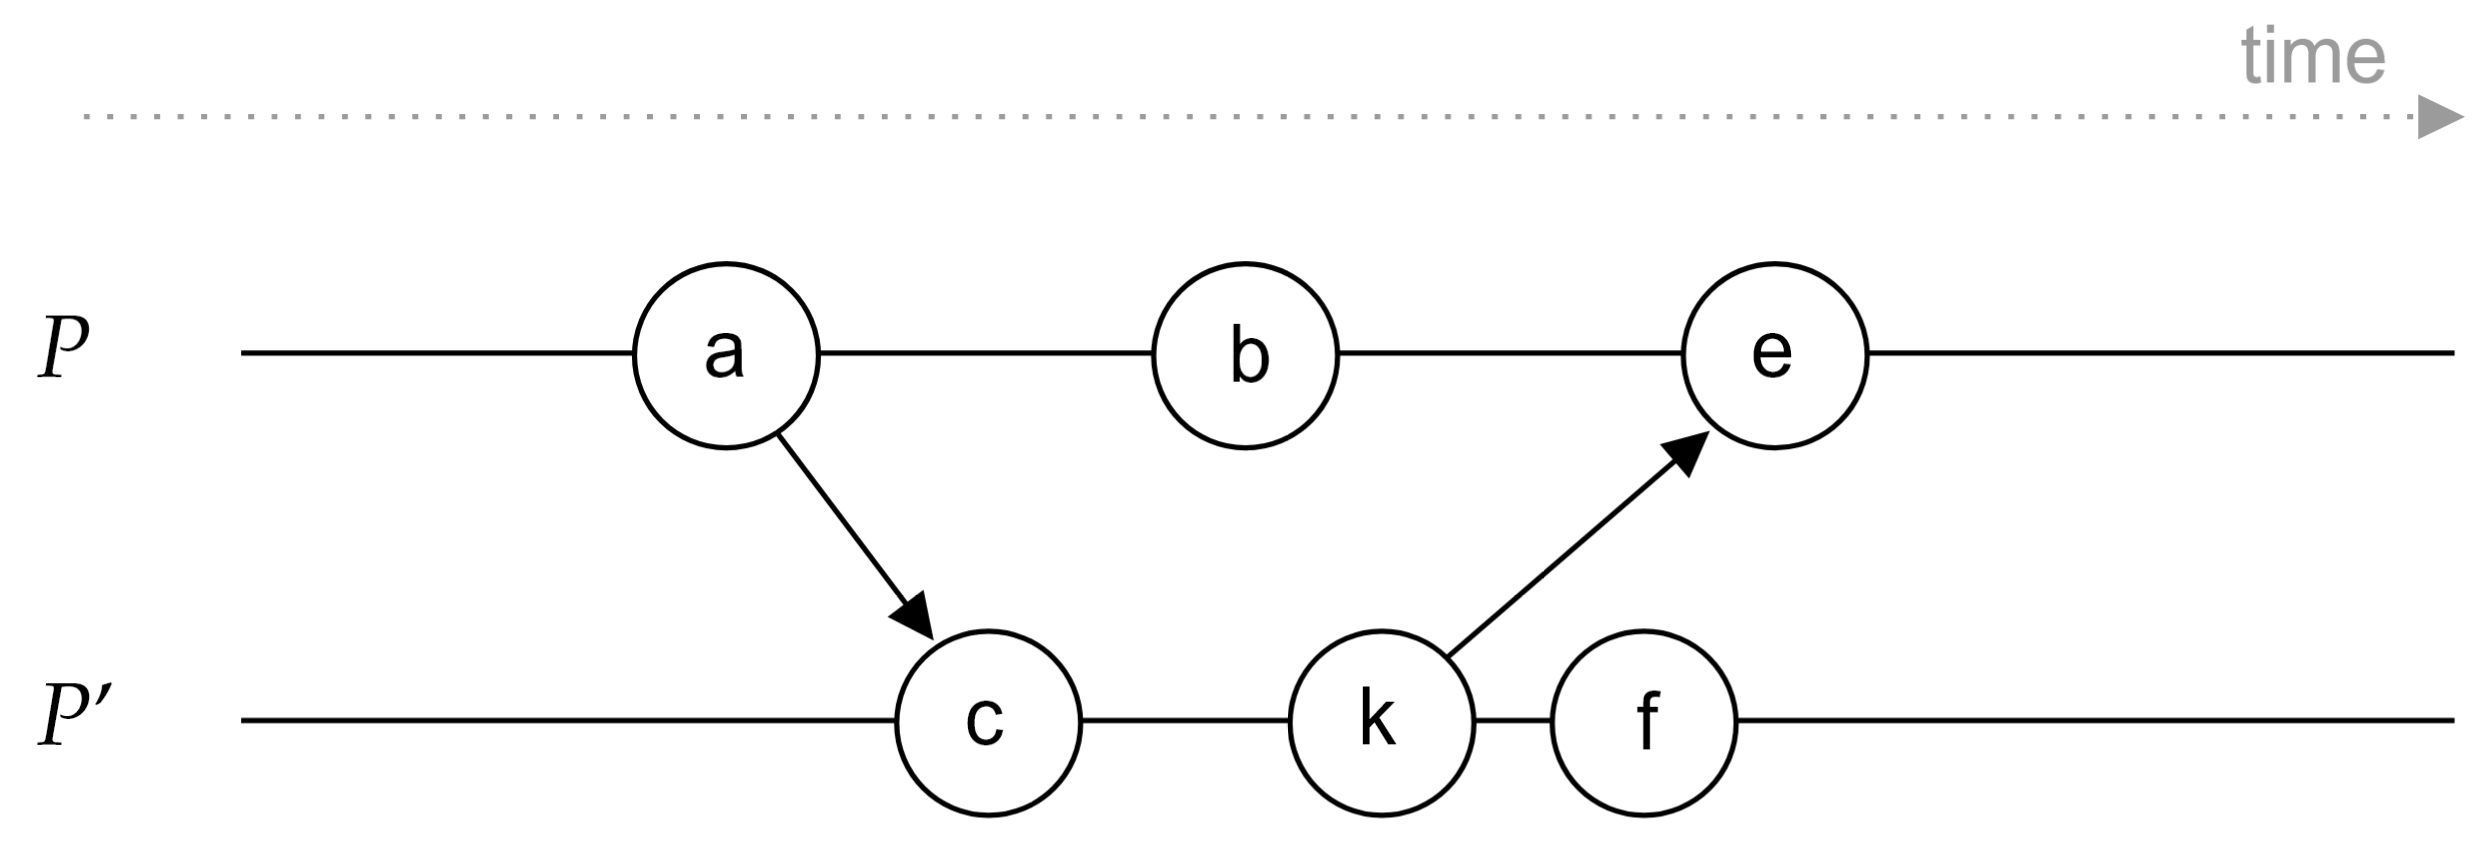
\includegraphics[width=.7\textwidth]{./Sections/time/causal.png}
        
    \vspace{1em}
    \noindent
    Answer on the next page.
\end{Example}
\newpage 

\noindent
\textbf{Example (\ref{ex:causal}) Answer:} (a): $a \rightarrow_r b$;\quad (b): $a \rightarrow_r k$;\quad (c): $c \parallel b$;\quad (d): $c \rightarrow_r e$.\\
\noindent
\rule{\textwidth}{0.4pt}\\

\noindent
Now we discuss a method that utilizes causal order, though assigns logical timestamps to events:
\begin{Def}[Lamport Clocks]

    Named after Leslie Lamport, Lamport Clocks assign a logical timestamp to each event:\\
    
    \noindent
    Let $t_p$ store the logical time of process $p$. Then,
    \begin{itemize}
        \item \textbf{Initialization:} $t_p$ is initialized to 0.
        \item \textbf{Timestamp Syntax:} Timestamps are tuples $(t_p, p)$, assigned to each $e$ event.
        \item \textbf{Incrementing:} For each $e$ in process $p$, increment $t_p$ by 1 and assign the $(t_p, p)$ to $e$.
        \item \textbf{Sending:} If $p$ sends a message $m$ to process $q$, the timestamp included is $((t_p+1), p)$.
        \item \textbf{Receiving:} Upon receiving message $m$, process $q$ sets $t_q = \max((t_p+1),t_q)$.
    \end{itemize}
\end{Def}

\begin{Example}[Lamport Clocks Example (\ref{ex:causal}) Extended]

    Consider the previous Example (\ref{ex:causal}) with Lamport Clocks:

    \hspace{4em}
    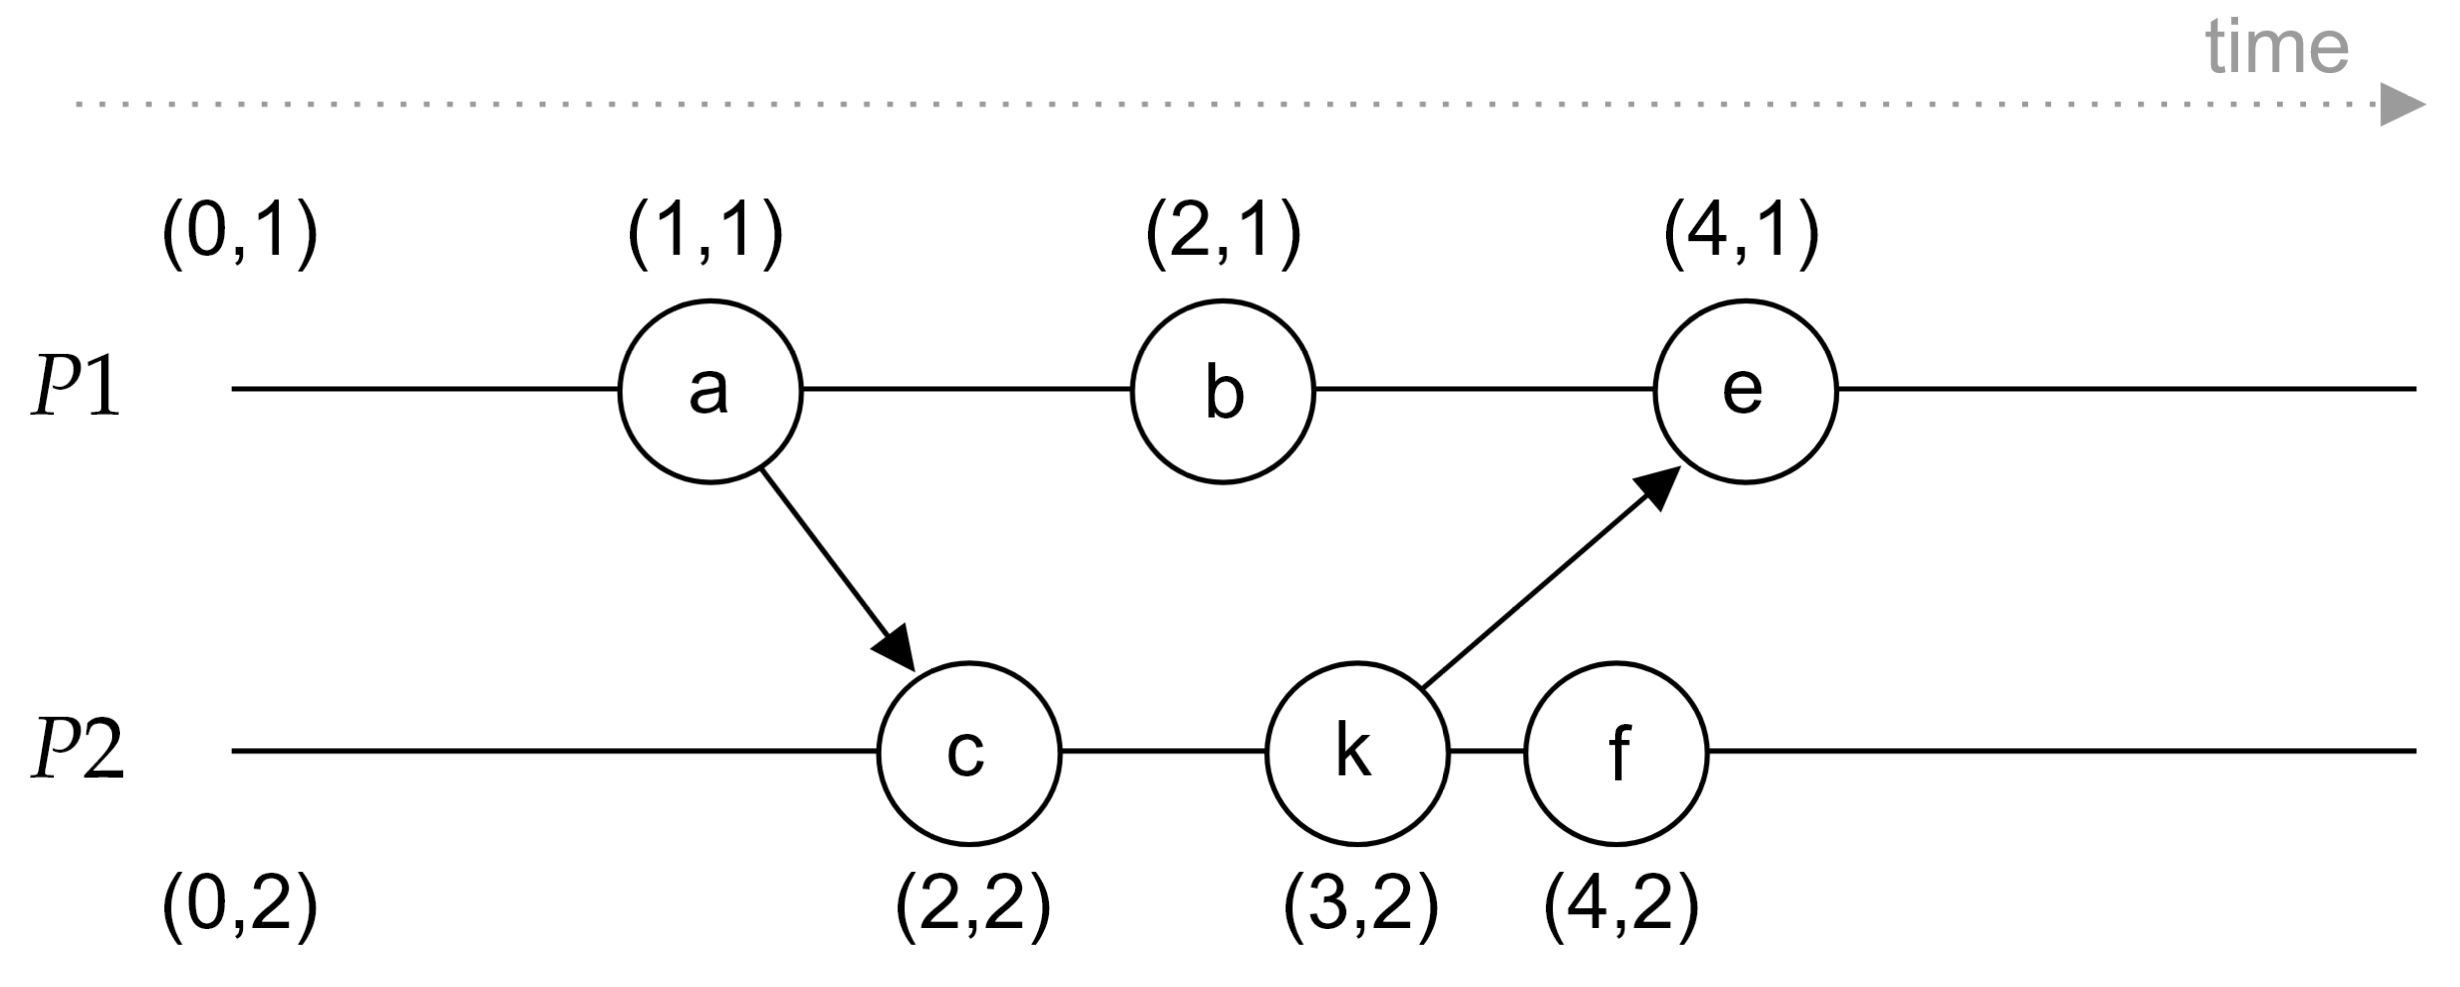
\includegraphics[width=.7\textwidth]{./Sections/time/lamport.png}

\end{Example}

\noindent
In practice the only thing we have access to are these logical timestamps, which we must evaluate:
\begin{theo}[Comparing Lamport Timestamps Causalaity]

    Given two events $a$ and $b$ with timestamps $t(a)$ and $t(b)$, with $r$ trace, we only guarantee:
    \begin{itemize}
        \item If $a \rightarrow_r b$, then $t(a) < t(b)$.
        \item If $t(a) \geq t(b)$, then $a \not\rightarrow_r b$.
    \end{itemize}
\end{theo}

\newpage 

\noindent
We may now derive the following about concurrency:
\begin{theo}[Non-causality]

    Two events $a$ and $b$ are concurrent ($a \parallel b$) under $r$ trace if \textbf{both} conditions 
    hold:
    \begin{itemize}
        \item $a \not\rightarrow_r b$ ($a$ does not happen before $b$).
        \item $b \not\rightarrow_r a$ ($b$ does not happen before $a$).
    \end{itemize}
\end{theo}

\noindent
Lamport Clocks are useful for causal ordering, but they do not capture the full context of events:
\begin{Def}[Vector Clocks]

   Let there be $p_1, p_2, \ldots, p_n$ processes each with a vector (array) $v$ of size $n$. Index $v_i[i]$ stores the logical time of process $p_i$.
   Then, the following rules apply:
   \begin{itemize}
    \item \textbf{Initialization:} Each $\ell\in v_i$ of $p_i$ is initialized to 0 (e.g., $[0,0,\dots,0]$).
    \item \textbf{Incrementing:} For each event $e$ in process $p_i$, increment $v_i[i]$ by 1.
    \item \textbf{Sending:} When $p_i$ sends a message $m$ to $p_j$, include $v_i$ in $m$ (\textbf{no increment}).
    \item \textbf{Receiving:} Upon receiving message $m$, process $p_j$ sets $v_j[j] = \max(v_j[j], v_i[j])$.
   \end{itemize}
\end{Def}

\begin{Example}[Vector Clocks Example]

    Observe the following events and their corresponding vector clocks:\\

    \hspace{4em}
    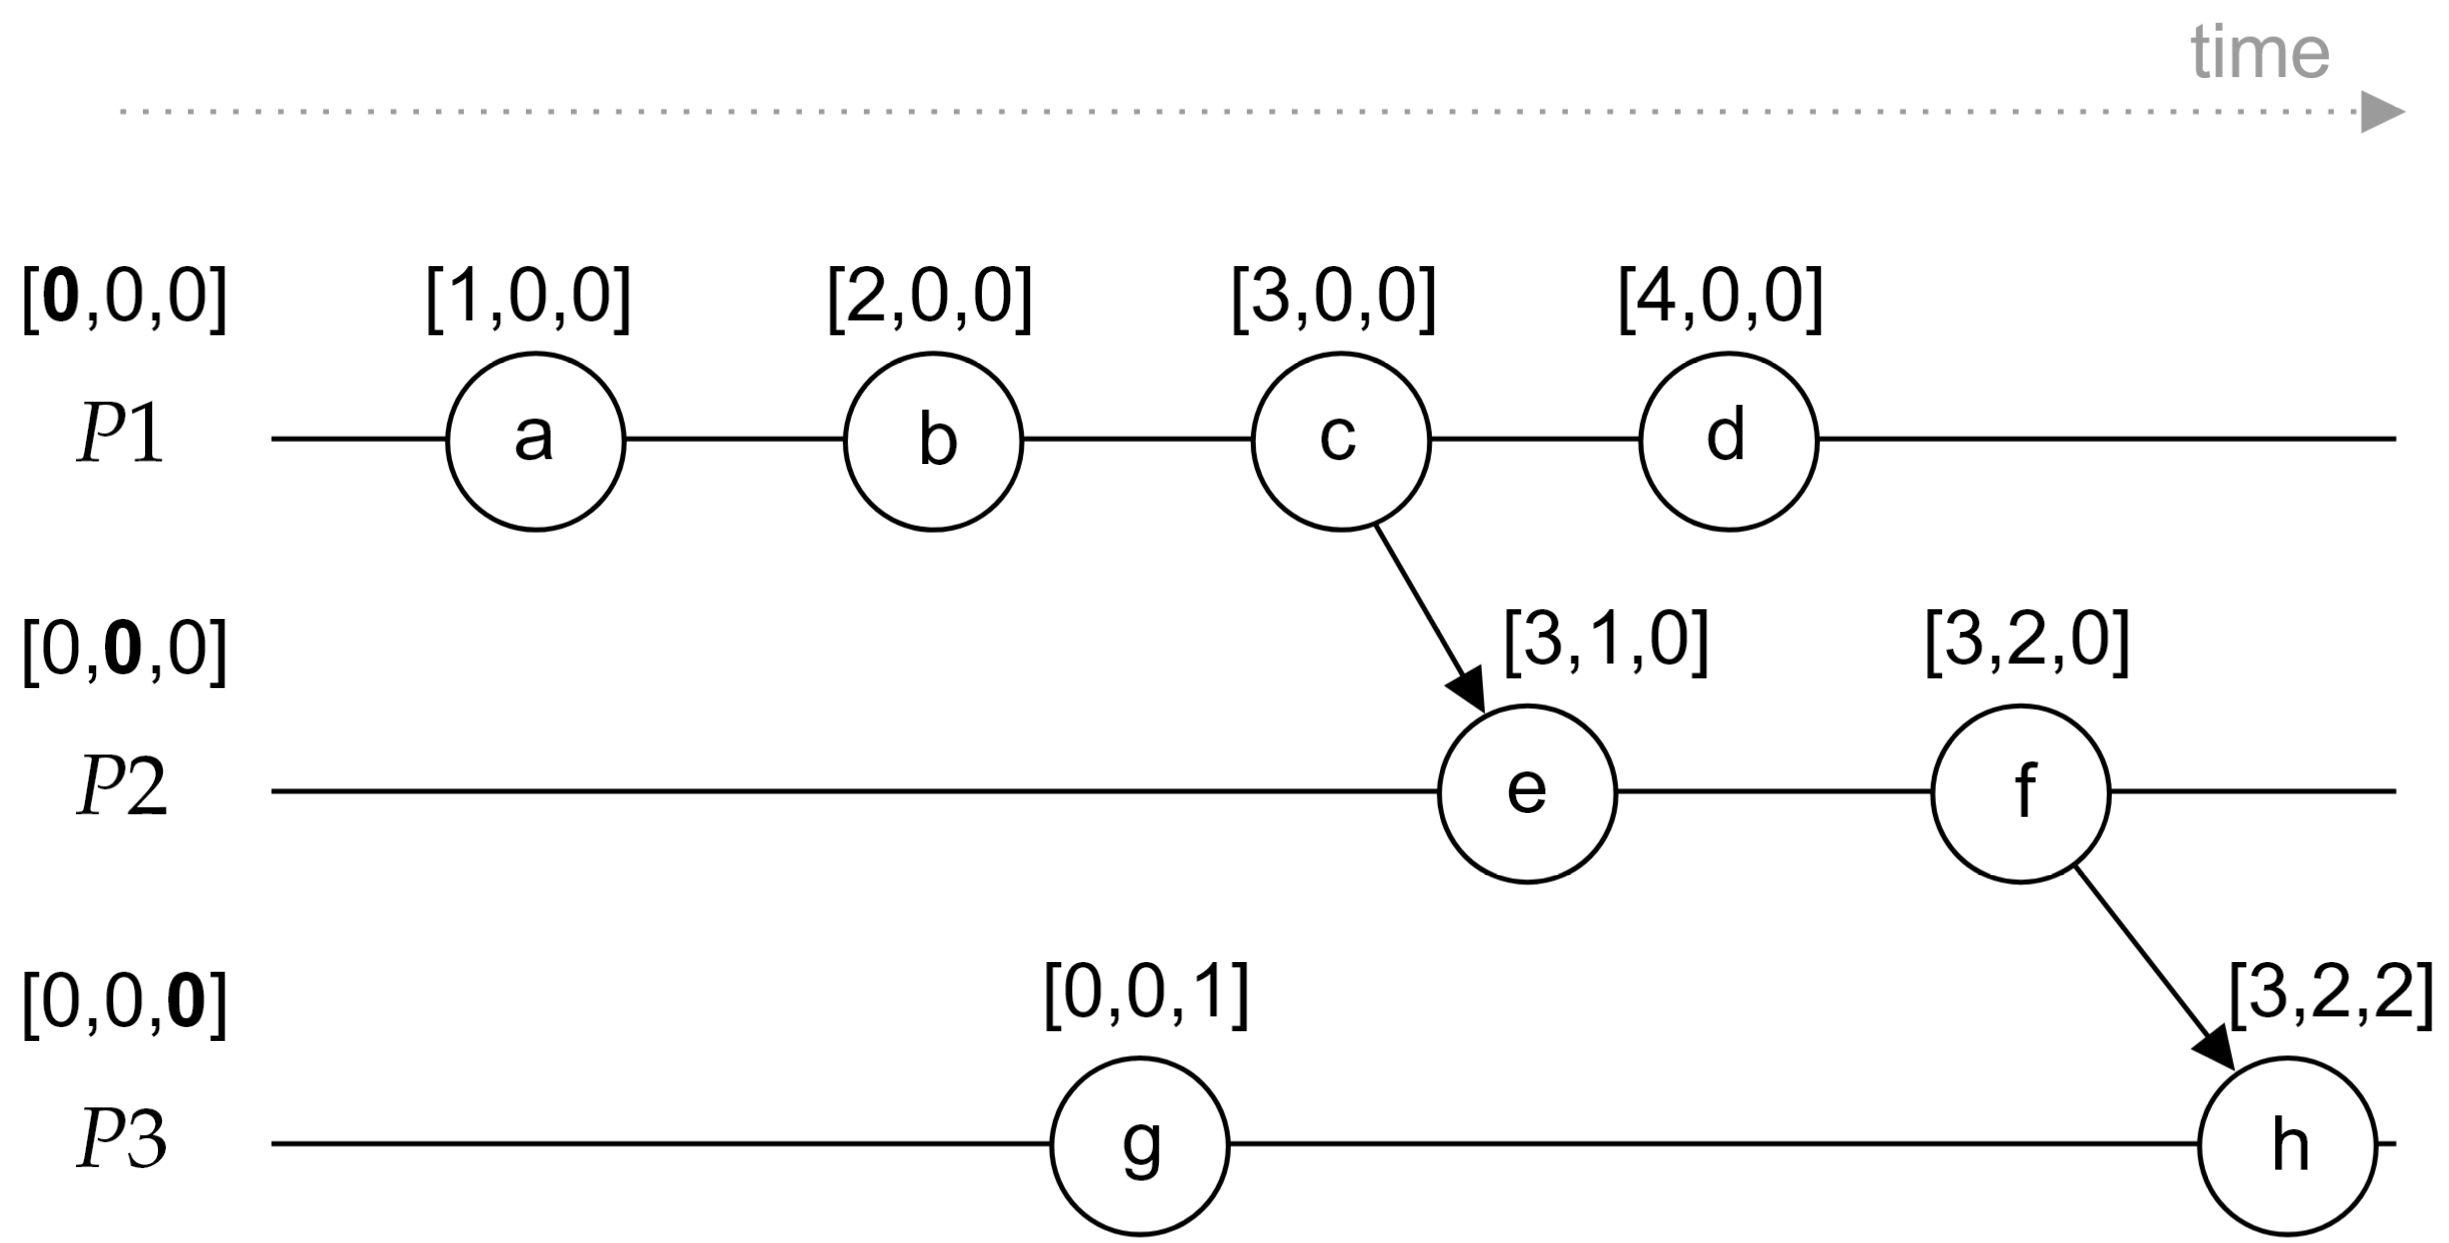
\includegraphics[width=.7\textwidth]{./Sections/time/vector.png}

    \vspace{1em}

\end{Example}

\newpage 

\noindent
There too is a method of comparing vector clocks:
\begin{theo}[Comparing Vector Clocks]

    Given two vectors $v_p$ and $v_q$ for processes $p$ and $q$, we may derive the following:
    \begin{itemize}
        \item $v_p \leq v_q \Longleftrightarrow \forall \ell:  v_p[\ell] \leq v_q[\ell]$
        \item $v_p < v_q \Longleftrightarrow \forall \ell:  v_p[\ell] < v_q[\ell]$
        \item $v_p <> v_q \text{ (non-comparable) } \Longleftrightarrow \forall \ell:  \neg(v_p < v_q ) \land \neg(v_p > v_q)$
    \end{itemize}

    \noindent
    i.e.,
    \begin{itemize}
        \item $v_p \leq v_q$: if and only if all corresponding indexes in $v_p$ are less than or equal to $v_q$.
        \item $v_p < v_q$: if and only if all corresponding indexes in $v_p$ are less than $v_q$.
        \item $v_p <> v_q$: if and only if there are at least two element pairs between $v_p$ and $v_q$ that are greater and less than each other.
        (e.g., $v_p = [1,2]$ and $v_q = [2,1]$, as $1 < 2$ and $2 > 1$).
    \end{itemize}
\end{theo}

\noindent
And for causality we have:
\begin{theo}[Vector Clocks Causality]

    Given two events $a$ and $b$ with vector clocks $v(a)$ and $v(b)$, we may derive the following:
    \begin{itemize}
        \item If $v(a) < v(b)$, then $a \rightarrow_r b$.
        \item If $a \rightarrow_r b$, then $v(a) < v(b)$.
    \end{itemize}
\end{theo}

\noindent
\rule{\textwidth}{0.4pt}\\

\begin{Exercise} Given the following Lamport timestamps, determine the causal order relationships:

    \begin{itemize}
        \item[(a)] $(0,P)\ ?\ (0,Q)$
        \item[(b)] $(1,P)\ ?\ (0,Q)$
        \item[(c)] $(0,P)\ ?\ (1,Q)$
    \end{itemize}
\end{Exercise}

\begin{Exercise} Given the following Vector clocks, determine the causal order relationships:

    \begin{itemize}
        \item[(a)] $[0,0]\ ?\ [0,0]$
        \item[(b)] $[1,0]\ ?\ [0,0]$
        \item[(c)] $[0,1]\ ?\ [1,0]$
    \end{itemize}
\end{Exercise}

\hfill \textit{Answers on the next page.}\hfill \null

\newpage 

\begin{Answer} Given the following Lamport timestamps, determine the causal order relationships:

    \begin{itemize}
        \item[(a)] $(0,P)\ ?\ (0,Q)$: $P \parallel Q$. To break the tie, the processes would need some order, say $(0,1)\rightarrow(0,2)$, is a possibility, but not guaranteed.
        \item[(b)] $(1,P)\ ?\ (0,Q)$: $P \parallel Q$ or $Q \rightarrow P$ are possible.
        \item[(c)] $(0,P)\ ?\ (1,Q)$: $Q \parallel P$ or $P \rightarrow Q$ are possible.
    \end{itemize}

    \noindent
    \textbf{Note:} The Lamport timestamps are not enough to determine causal order relationships between independent processes, unless 
    we have the context of the execution trace. In the processes were orderd
\end{Answer}

\begin{Answer} Given the following Vector clocks, determine the causal order relationships:

    \begin{itemize}
        \item[(a)] $[0,0]\ ?\ [0,0]$: $[0,0] \parallel [0,0]$
        \item[(b)] $[1,0]\ ?\ [0,0]$: $[1,0] \not\rightarrow [0,0]$
        \item[(c)] $[0,1]\ ?\ [1,0]$: $[0,1] <> [1,0]$ or $[0,1] \parallel [1,0]$
    \end{itemize}
\end{Answer}
% \newpage 
\section{Implementing RPCs with Go}
Before we can make RPC calls in Go, we need to understand Go's typing system.
\subsection{Typing in Go}

\begin{Def}[Typing in Go]

    Go is a statically typed language, meaning every variable has a fixed type at compile time. The language provides several built-in types, including:
\textbf{Basic Types:} \snippet{int}, \snippet{float64}, \snippet{string}, \snippet{bool}, and \textbf{Composite Types:} \snippet{array}, \snippet{slice}, \snippet{map}, \snippet{struct}, \snippet{interface}.
    
    A \textbf{type} in Go can also be user-defined using the \snippet{type} keyword. For example, we can define a custom structure:
    
    \begin{lstlisting}[language=Go, numbers=none]
    type Person struct {
        Name string
        Age  int
    }
    \end{lstlisting}
    
    A \snippet{struct} groups related fields together, allowing us to represent objects with multiple attributes. We can create and use instances of this struct:
    
    \begin{lstlisting}[language=Go, numbers=none]
    p := Person{Name: "Alice", Age: 25}
    fmt.Println(p.Name) // Outputs: Alice
    \end{lstlisting}
   
\end{Def}
    
\begin{Def}[Typing Functions in Go]

    Functions are explicitly typed, meaning parameters and return values must be declared:
    
    \begin{lstlisting}[language=Go, numbers=none]
    // Takes two ints and returns an int
    func Add(x int, y int) int { 
        return x + y
    }

    // We can shorthand parameters of the same type:
    func Divide(x, y int) (int, error) { // Returns an int and an error
        if y == 0 {
            return 0, fmt.Errorf("division by zero")
        }
        return x / y, nil
    }
    \end{lstlisting}
    
    \noindent
    Here, \snippet{fmt.Errorf()} generates an error message.
    
\end{Def}
    
\begin{Def}[Methods in Go: Pointers vs. Values]

    In Go, methods can be defined for both pointer receivers (\snippet{*T}) and value receivers (\snippet{T}). A method with a pointer receiver can modify the original struct, while a method with a value receiver works on a copy.
    Consider a struct representing a rectangle:
    
    \begin{lstlisting}[language=Go, numbers=none]
    package main; import "fmt"

    type rect struct {
        width, height int
    }
    
    // Pointer receiver: Can modify the original struct
    func (r *rect) area() int {
        return r.width * r.height
    }
    
    // Value receiver: Works on a copy of rect
    func (r rect) perim() int {
        return 2*r.width + 2*r.height
    }
    
    func (r *rect) setWidth(w int) {
        r.width = w
    }
    
    func (r rect) setHeight(h int) {
        r.height = h
    }
    
    func main() {
        
        r := rect{width: 10, height: 5}
        // Converts r.area() to (&r).area() automatically
        fmt.Println("area: ", r.area())  // 50
        fmt.Println("perim:", r.perim()) // 30
    
        rp := &r
        // Converts rp.perim() to (*rp).perim() automatically
        fmt.Println("perim:", rp.perim()) // 30
        fmt.Println("area: ", rp.area())  // 50
    
        r.setWidth(20)
        r.setHeight(10)
        fmt.Println("width:", r.width) // 20
        fmt.Println("height:", r.height) // 5
    }
    \end{lstlisting}
    
    \end{Def}
    
    \newpage 

    \subsection{Go's RPC Package}
    In Go, we can use the \snippet{net/rpc} package to implement server-clint RPCs.

    \begin{Def}[Setting Up an RPC Server and Client in Go]
    
    \noindent
    \textbf{Setting Up an RPC Server}:
    To create an RPC server in Go, we need to,
    \begin{itemize}
        \item Define a \textbf{service type} (a struct) that will handle remote calls.
        \item Implement \textbf{methods} that satisfy the RPC requirements.
        \item Register the service using \snippet{rpc.Register()}.
        \item Set up a network listener using \snippet{net.Listen()}.
        \item Handle requests using \snippet{rpc.HandleHTTP()} and \snippet{http.Serve()}.
    \end{itemize}
    
    \noindent
    \textbf{RPC Method Requirements}:
    Methods must satisfy these constraints or be ignored:
    \begin{itemize}
        \item The method itself and its \textbf{type} must be exported.
        \item The method must return a single value of type \snippet{error}, and have exactly \textbf{two arguments}, both of which must be \textbf{exported or built-in types}.
        \item The method's \textbf{second argument must be a pointer}.
    \end{itemize}
    
    \noindent
    E.g. Signature,
    
    \begin{lstlisting}[language=Go, numbers=none]
    func (t *T) MethodName(argType T1, replyType *T2) error
    \end{lstlisting}
    
    \noindent
    \textbf{Setting Up an RPC Client}:
    To communicate with the RPC server, a client must,
    \begin{itemize}
        \item Establish a connection using \snippet{rpc.DialHTTP()}.
        \item Call remote methods synchronously with \snippet{client.Call()}.
        \item Call remote methods asynchronously with \snippet{client.Go()}.
    \end{itemize}
    \end{Def}

    \begin{Example}[Simple Local Arithmetic RPC (Part 1)]
        Let's create a simple Arithmetic RPC. First let's setup our file structure:\\
    \noindent
    \rule {.9\textwidth}{0.5pt}
    
        \dirtree{%
        .1 arith/.
        .2 server/.
        .3 server.go.
        .2 client.go.
        }
    \noindent
        \rule {.9\textwidth}{0.5pt}
\end{Example}
        
\newpage 

\vspace{-1em}
\begin{Example}[Simple Local Arithmetic RPC (Part 2)]

    Now to setup the server:
    \begin{lstlisting}[language=Go, numbers=none]
package main; import "fmt"; import "log"; import "net"; import "net/rpc"

    type ArithService int  // Define the service type

    type Args struct {  A, B int } // Define the arguments struct

    type Quotient struct { Quo, Rem int } // Reply struct for Dividing

    // Both Multiply and Divide methods satisfy the RPC requirements
    func (t *ArithService) Multiply(args *Args, reply *int) error {
        *reply = args.A * args.B
        return nil
    }

    func (t *ArithService) Divide(args *Args, quo *Quotient) error {
        if args.B == 0 { return fmt.Errorf("divide by zero")}
        quo.Quo = args.A / args.B
        quo.Rem = args.A % args.B
        return nil
    }

    func main() {
        arith := new(ArithService)
        err := rpc.Register(arith)
        if err != nil { log.Fatal("Register Error:", err) }

        listener, err := net.Listen("tcp", ":8080")
        if err != nil { log.Fatal("RPC Start Error:", err)}

        defer listener.Close()
        log.Println("Arithmetic RPC server is running on port 8080")

        for {
            // Server waits until a connection is made
            conn, err := listener.Accept()
            if err != nil {
                log.Println("Connection Error:", err)
                continue
            }
            // Serves the connection on a new goroutine
            go rpc.ServeConn(conn)
        }
    }
    \end{lstlisting}
    \end{Example}

\newpage 

\begin{Example}[Simple Local Arithmetic RPC (Part 3)]

    After the following client code, run the server first, then client on a separate terminals:
    \begin{lstlisting}[language=Go, numbers=none]
    package main; import "fmt"; import "log"; import "net/rpc"
    
    // Define the same structures as the server
    type Args struct {
        A, B int
    }

    type Quotient struct {
        Quo, Rem int
    }

    func main() {
        // Connect to the RPC server
        client, err := rpc.Dial("tcp", "localhost:8080")
        if err != nil {
            log.Fatal("Error dialing:", err)
        }
        defer client.Close()

        // Perform a multiplication RPC call
        args := &Args{7, 8}
        var reply int
        err = client.Call("ArithService.Multiply", args, &reply)
        if err != nil {
            log.Fatal("Multiply error:", err)
        }

        // Perform a division RPC call
        var quotient Quotient
        err = client.Call("ArithService.Divide", args, &quotient)
        if err != nil {
            log.Fatal("Divide error:", err)
        }

        // Output: 7 * 8 = 56
        fmt.Printf("ArithService: %d * %d = %d\n", args.A, args.B, reply)

        // Output: 7 / 8 = 0, remainder = 7
        fmt.Printf("ArithService: %d / %d = %d, remainder = %d\n", args.A, args.B, quotient.Quo, quotient.Rem)
    }
    \end{lstlisting}
    \end{Example}

% \chapter{Working with Distributed Systems}
% \section{Saving System State: Snapshots}

\label{sec:snap}
This section discusses saving state. This is useful for fault-tolerance and system migrations.

\begin{Def}[Snapshot]
    
    \label{def:snapshot}
    A \textbf{snapshot} is a consistent global state of a distributed system at a specific point in time. 
\end{Def}

\begin{Def}[Consistent vs. Inconsistent Snapshots]

    To evaluate a snapshot's consistency, we compare events in the system \textbf{pre-snapshot} (events before the snapshot) 
    and \textbf{post-snapshot} (events after the snapshot). The snapshot itself is instantaneous, like a photograph. 
    Given an event ordering $r$:
    
    \begin{itemize}
        \item \textbf{Consistent Snapshots}: Respect causal dependencies. Let there be events $e_1$ and $e_2$; If $e_1 \rightarrow_r e_2$, then $e_1$ must be included in the snapshot if $e_2$ is present.
        \item \textbf{Inconsistent Snapshots}: Violate causal dependencies. If $e_2$ is included without 
        the causally preceding event $e_1$, then the snapshot is inconsistent.
    \end{itemize}
\end{Def}

\vspace{-1em}
\begin{figure}[h]
    \centering
    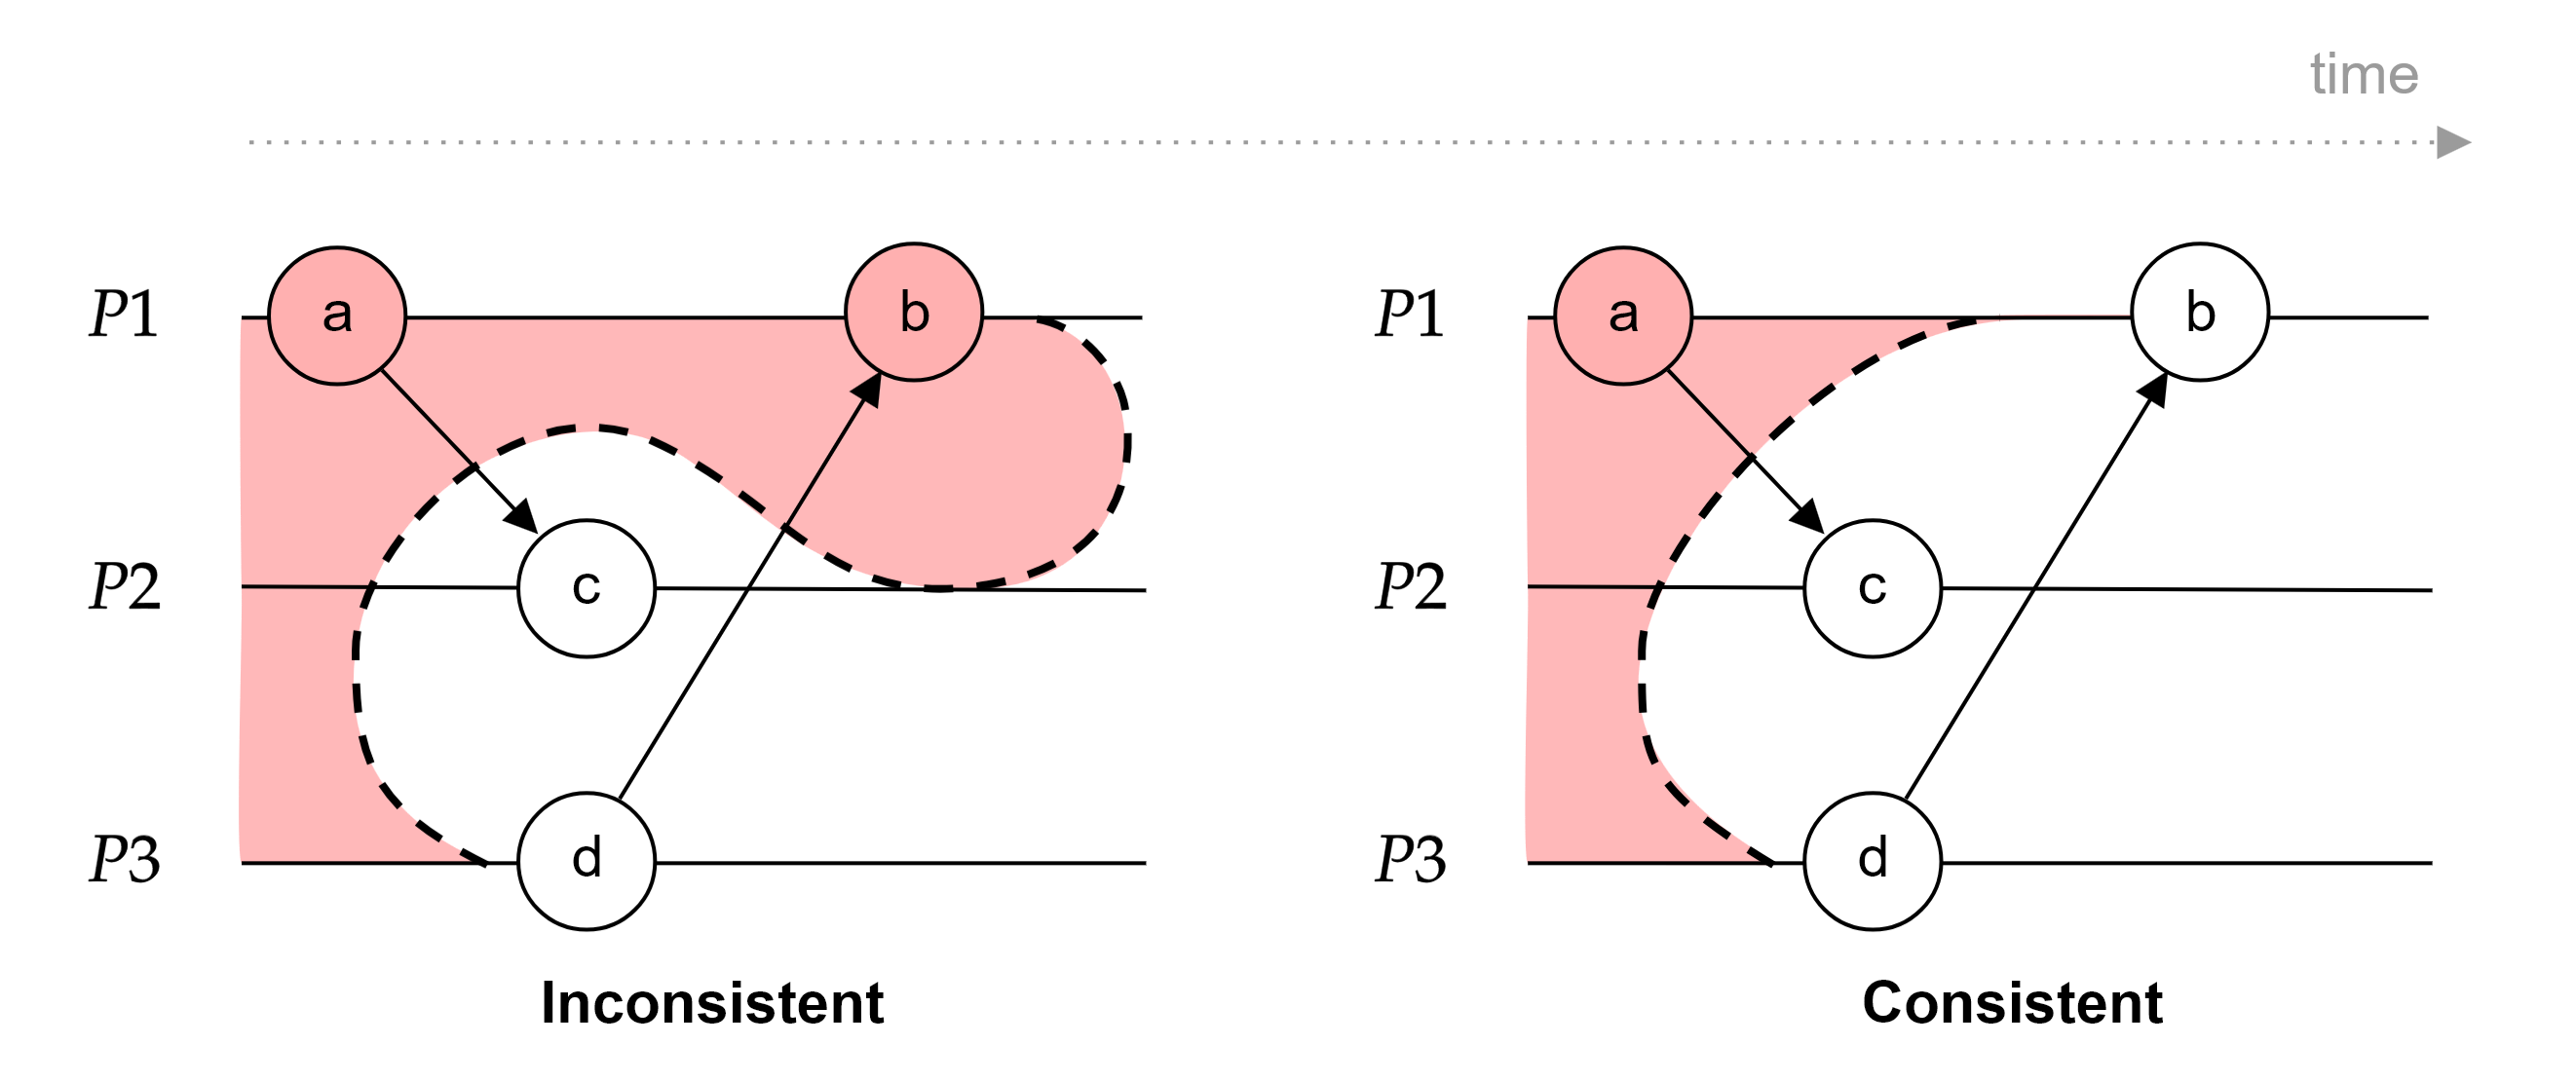
\includegraphics[width=.9\textwidth]{Sections/snap/snap.png}
    \caption{Inconsistent vs. Consistent Snapshots (pre-snapshot highlighted in red)}
\end{figure}

\noindent 
Here, in the inconsistent snapshot, $b$ is included without $d$, its causally preceding event. In the consistent snapshot, only $a$ is 
included. In this snapshot $c$ and $d$ could be added without violating causality.

\newpage 

\noindent 
There are many snapshot protocols, but we will focus on the \textbf{Chandy-Lamport Algorithm}.
\begin{Def}[Chandy-Lamport Algorithm]

    The \textbf{Chandy-Lamport Algorithm} is a snapshot algorithm that is used in distributed systems for
    recording a consistent global state of an asynchronous system. In this protocol:
    \begin{itemize}
        \item The snapshot procedure does not disrupt other processes.
        \item Each process records its local state.
        \item Any process can initiate the snapshot.
    \end{itemize}
    \noindent
    This model requires: 
    \begin{itemize}
        \item \textbf{No Failures}: No failures during the snapshot.
        \item \textbf{First in, First out Channels (FIFO)}: no lost or duplicated messages.
        \item \textbf{Strongly Connected Network}: All processes can reach every other process.
        \item \textbf{Single Initiator}: Only one process can initiate the snapshot.
    \end{itemize}
    
    \noindent 
    The initiator then:
    \begin{itemize}
        \item Sends a \textbf{Marker} message to all outgoing channels.
        \item Records local and incoming channel data.
    \end{itemize}
    Recipients of the marker message:
    \begin{itemize}
        \item Designates the channel which the marker arrived as \textbf{empty}.
        \item Records their local state and all other incoming channels \underline{except the empty one}.
        \item Sends the marker to all outgoing channels.
    \end{itemize}
    \noindent
    \textbf{Completion}: When all processes have received and sent a marker, the snapshot is complete. This 
    means every processes incoming channel is empty, hence the conclusion of the snapshot.
\end{Def}

\begin{Tip} Leslie Lamport recalls the Chandy-Lamport Algorithm's creation as follows:\\
    ``The distributed snapshot algorithm described here came
    about when I visited Chandy, who was then at the
    University of Texas in Austin. He posed the problem to me
    over dinner, but we had both had too much wine to think
    about it right then. The next morning, in the shower, I came
    up with the solution. When I arrived at Chandy's office, he
    was waiting for me with the same solution.''\\

    \noindent
    - \href{https://lamport.azurewebsites.net/pubs/chandy.pdf}{https://lamport.azurewebsites.net/pubs/chandy.pdf}
\end{Tip}

\newpage 

\noindent 
Observe the following illustration of the Chandy-Lamport Algorithm given processes $p_1, p_2, p_3$:
\begin{figure}[h] 
    \centering
    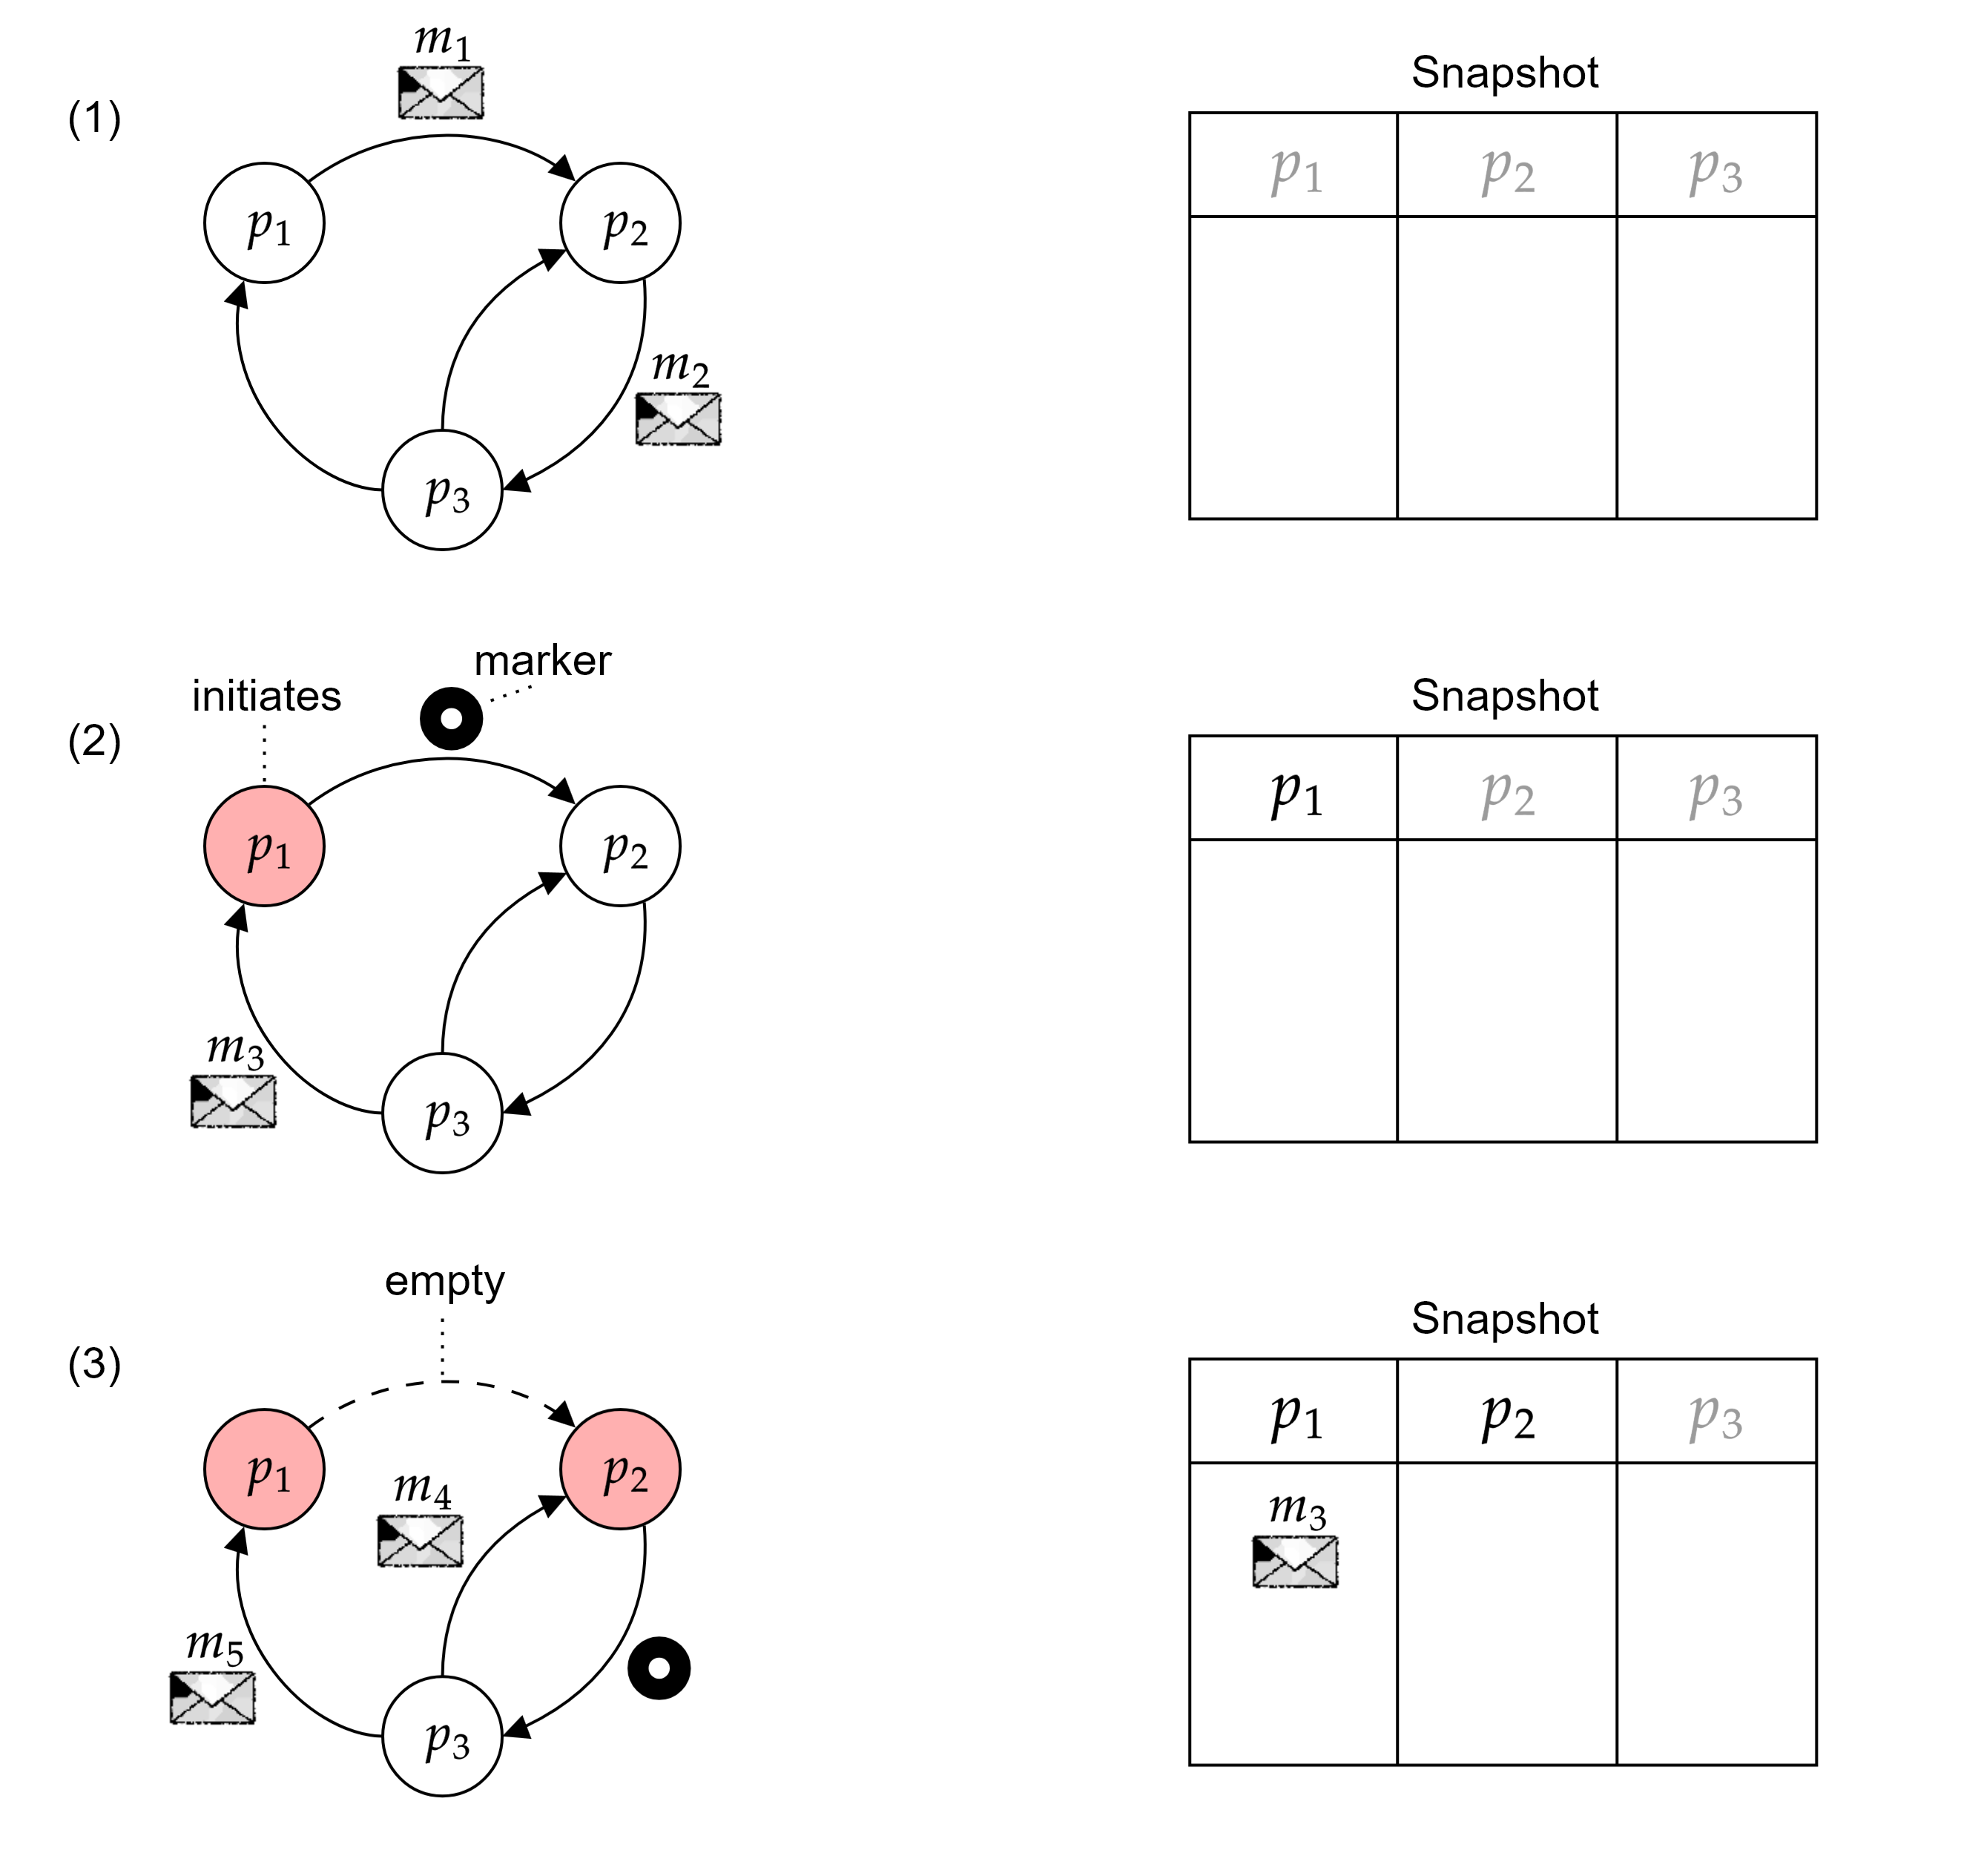
\includegraphics[width=1\textwidth]{Sections/snap/snap_exe.png}
\end{figure}

\noindent
Examining these first three steps: (1) The system before the snapshot. (2) $p_1$ initiates the snapshot sending a marker to $p_2$ and recording its local and incoming channel's state. 
(3) $p_2$ receives the marker, designating the incoming channel from $p_1$ as empty, sends the marker on outgoing channels, and begins recording. We also see, $p_1$ has recorded an incoming message $m_3$ from (2).\\

\noindent
We continue on the next page.

\newpage 

\noindent
We continue the snapshot process with the following steps:
\begin{figure}[h] 
    \centering
    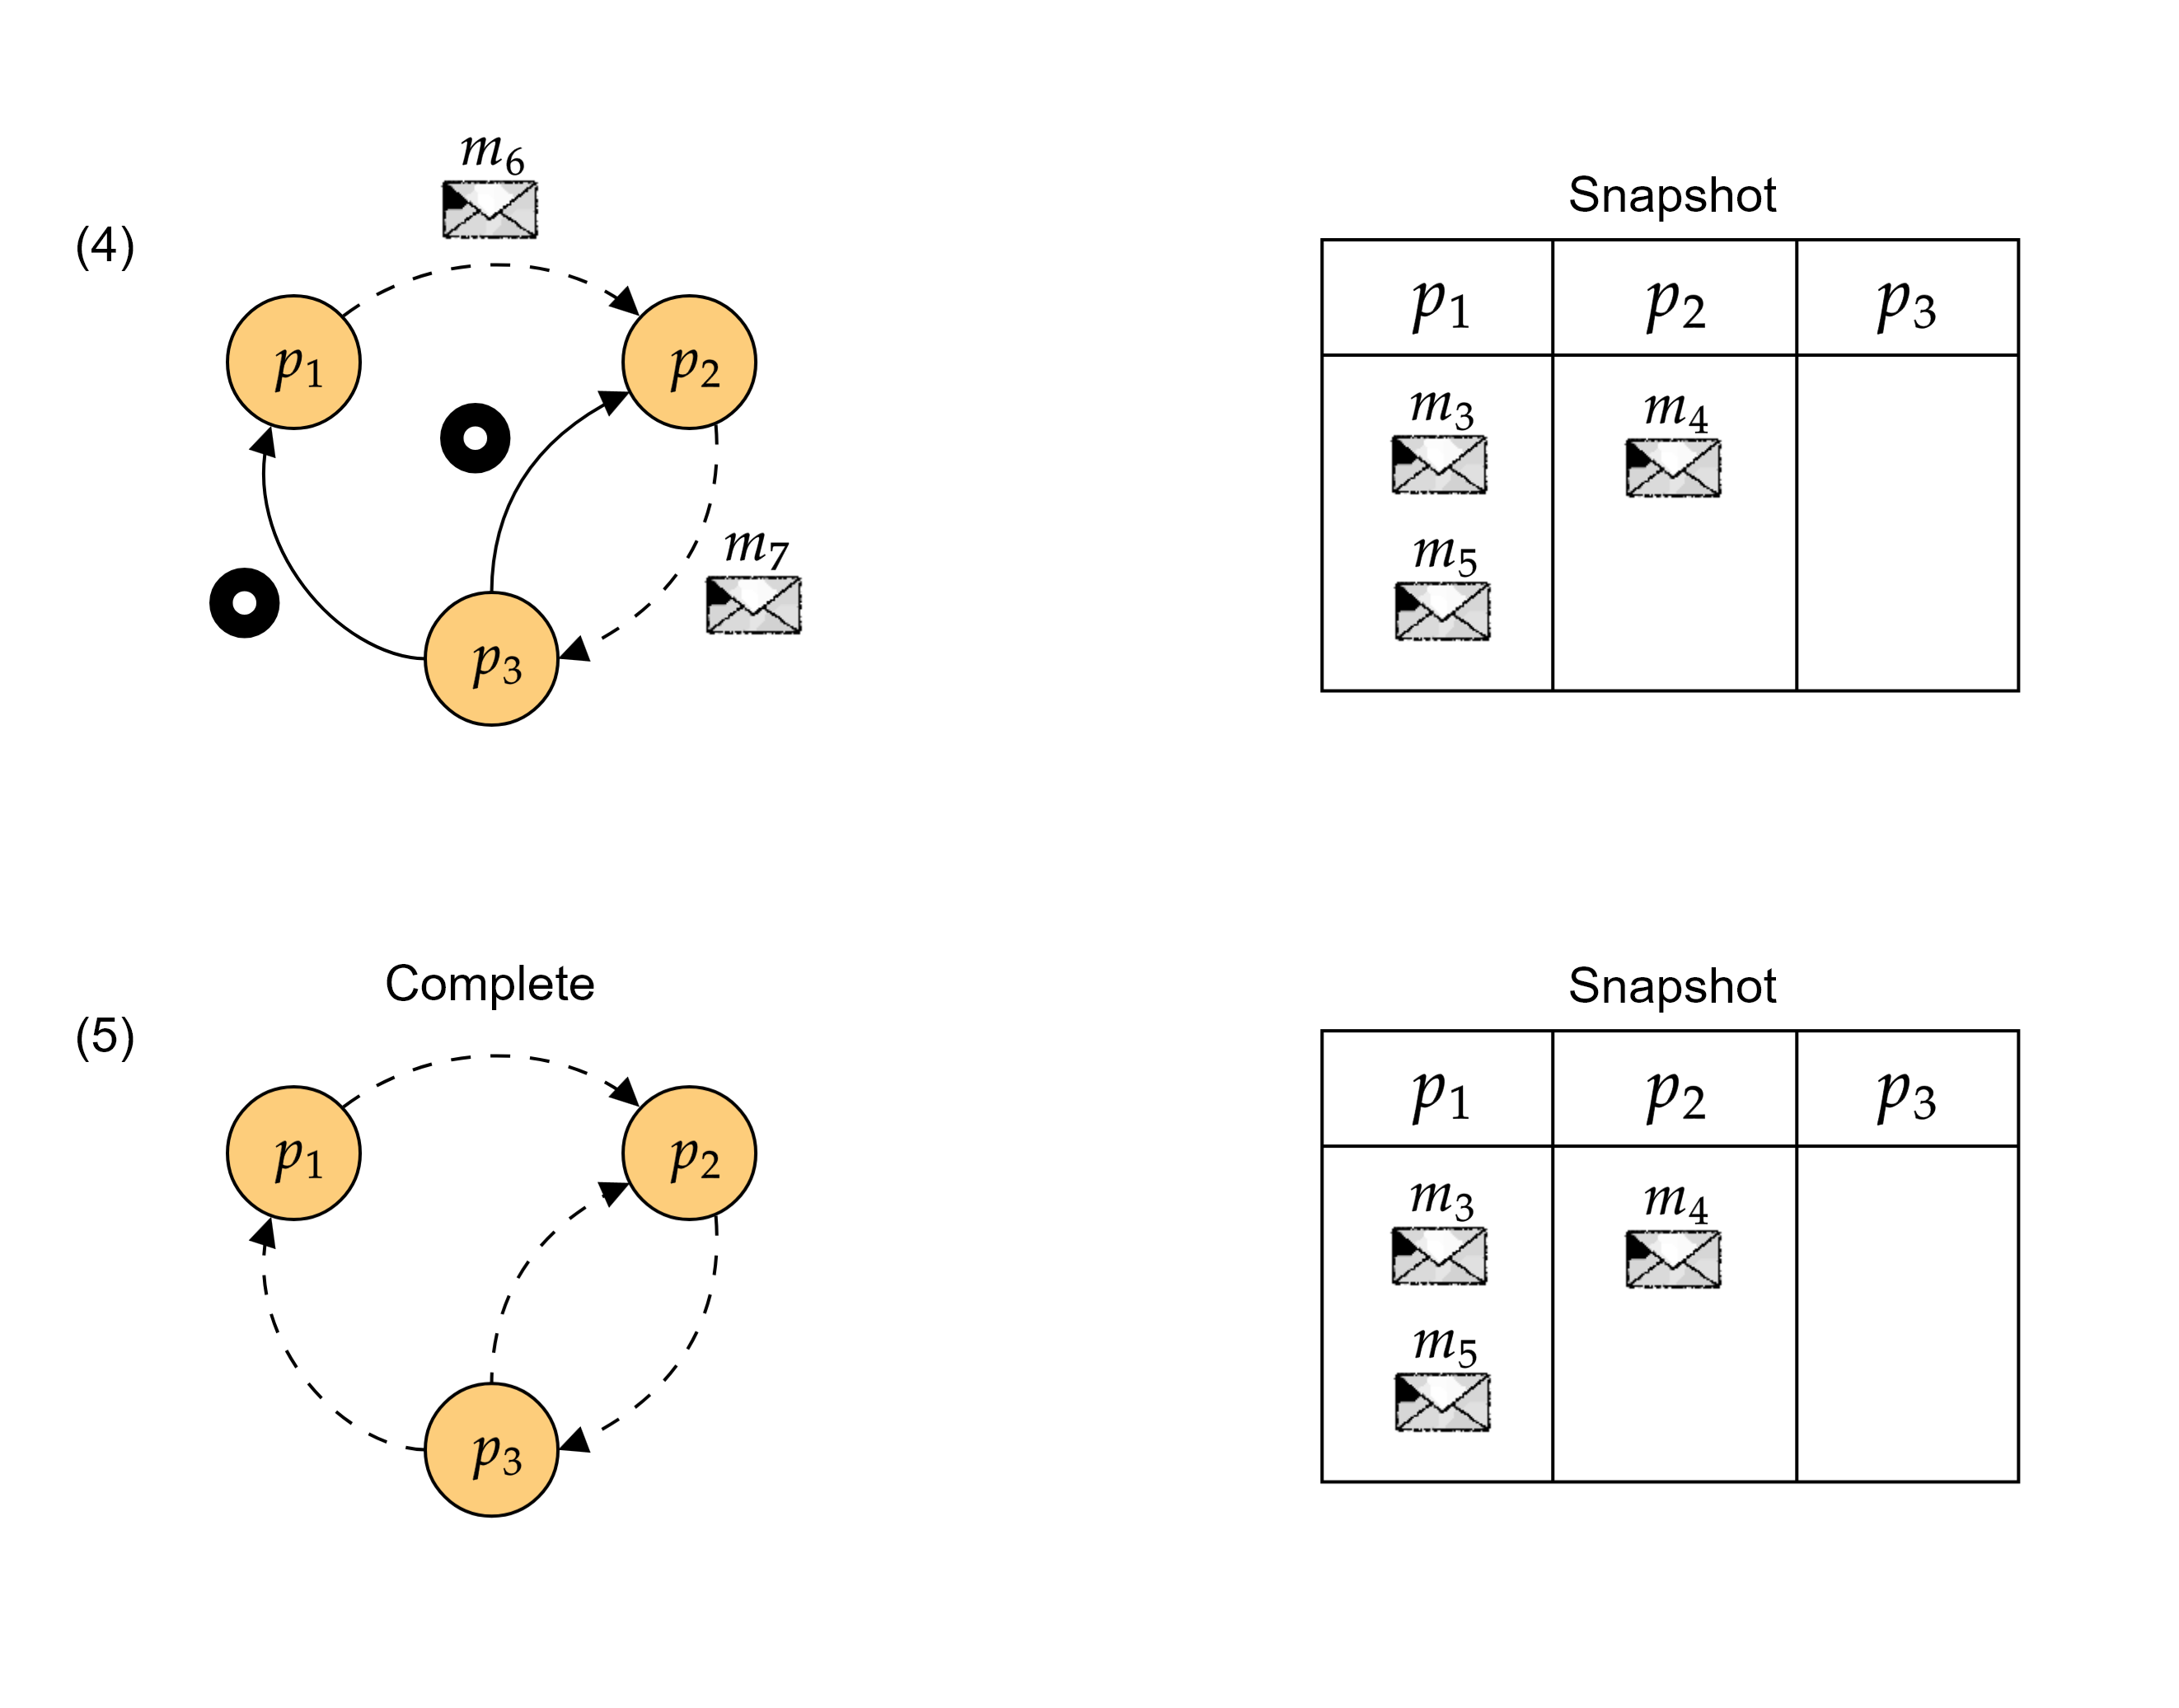
\includegraphics[width=1\textwidth]{Sections/snap/snap_exe_2.png}
\end{figure}

\noindent
(4) $p_3$ received the marker from $p_2$, and designates that incoming channel as empty. It begins recording state, sending out the marker to $p_1$ and $p_2$.
Take notice that messages $m_4$ and $m_5$ have been recorded from (3).
(5) All channels are now empty, concluding the snapshot. Take note that $m_6$ and $m_7$ were not recorded as they were sent on empty channels.
% \newpage
\section{Replication: Synchronizing State}

This section discusses replicating state across distributed systems.

\begin{Def}[Replication]

    \textbf{Replication} is the process of maintaining multiple copies of the same data on different nodes (machines). 
    This is done for fault-tolerance, load balancing, and data locality.
\end{Def}

\noindent
\textbf{Problem Space:}\\
Consider we are running a money transfer service, from which Alice and Bob interact with:
\begin{figure}[h]
    \centering
    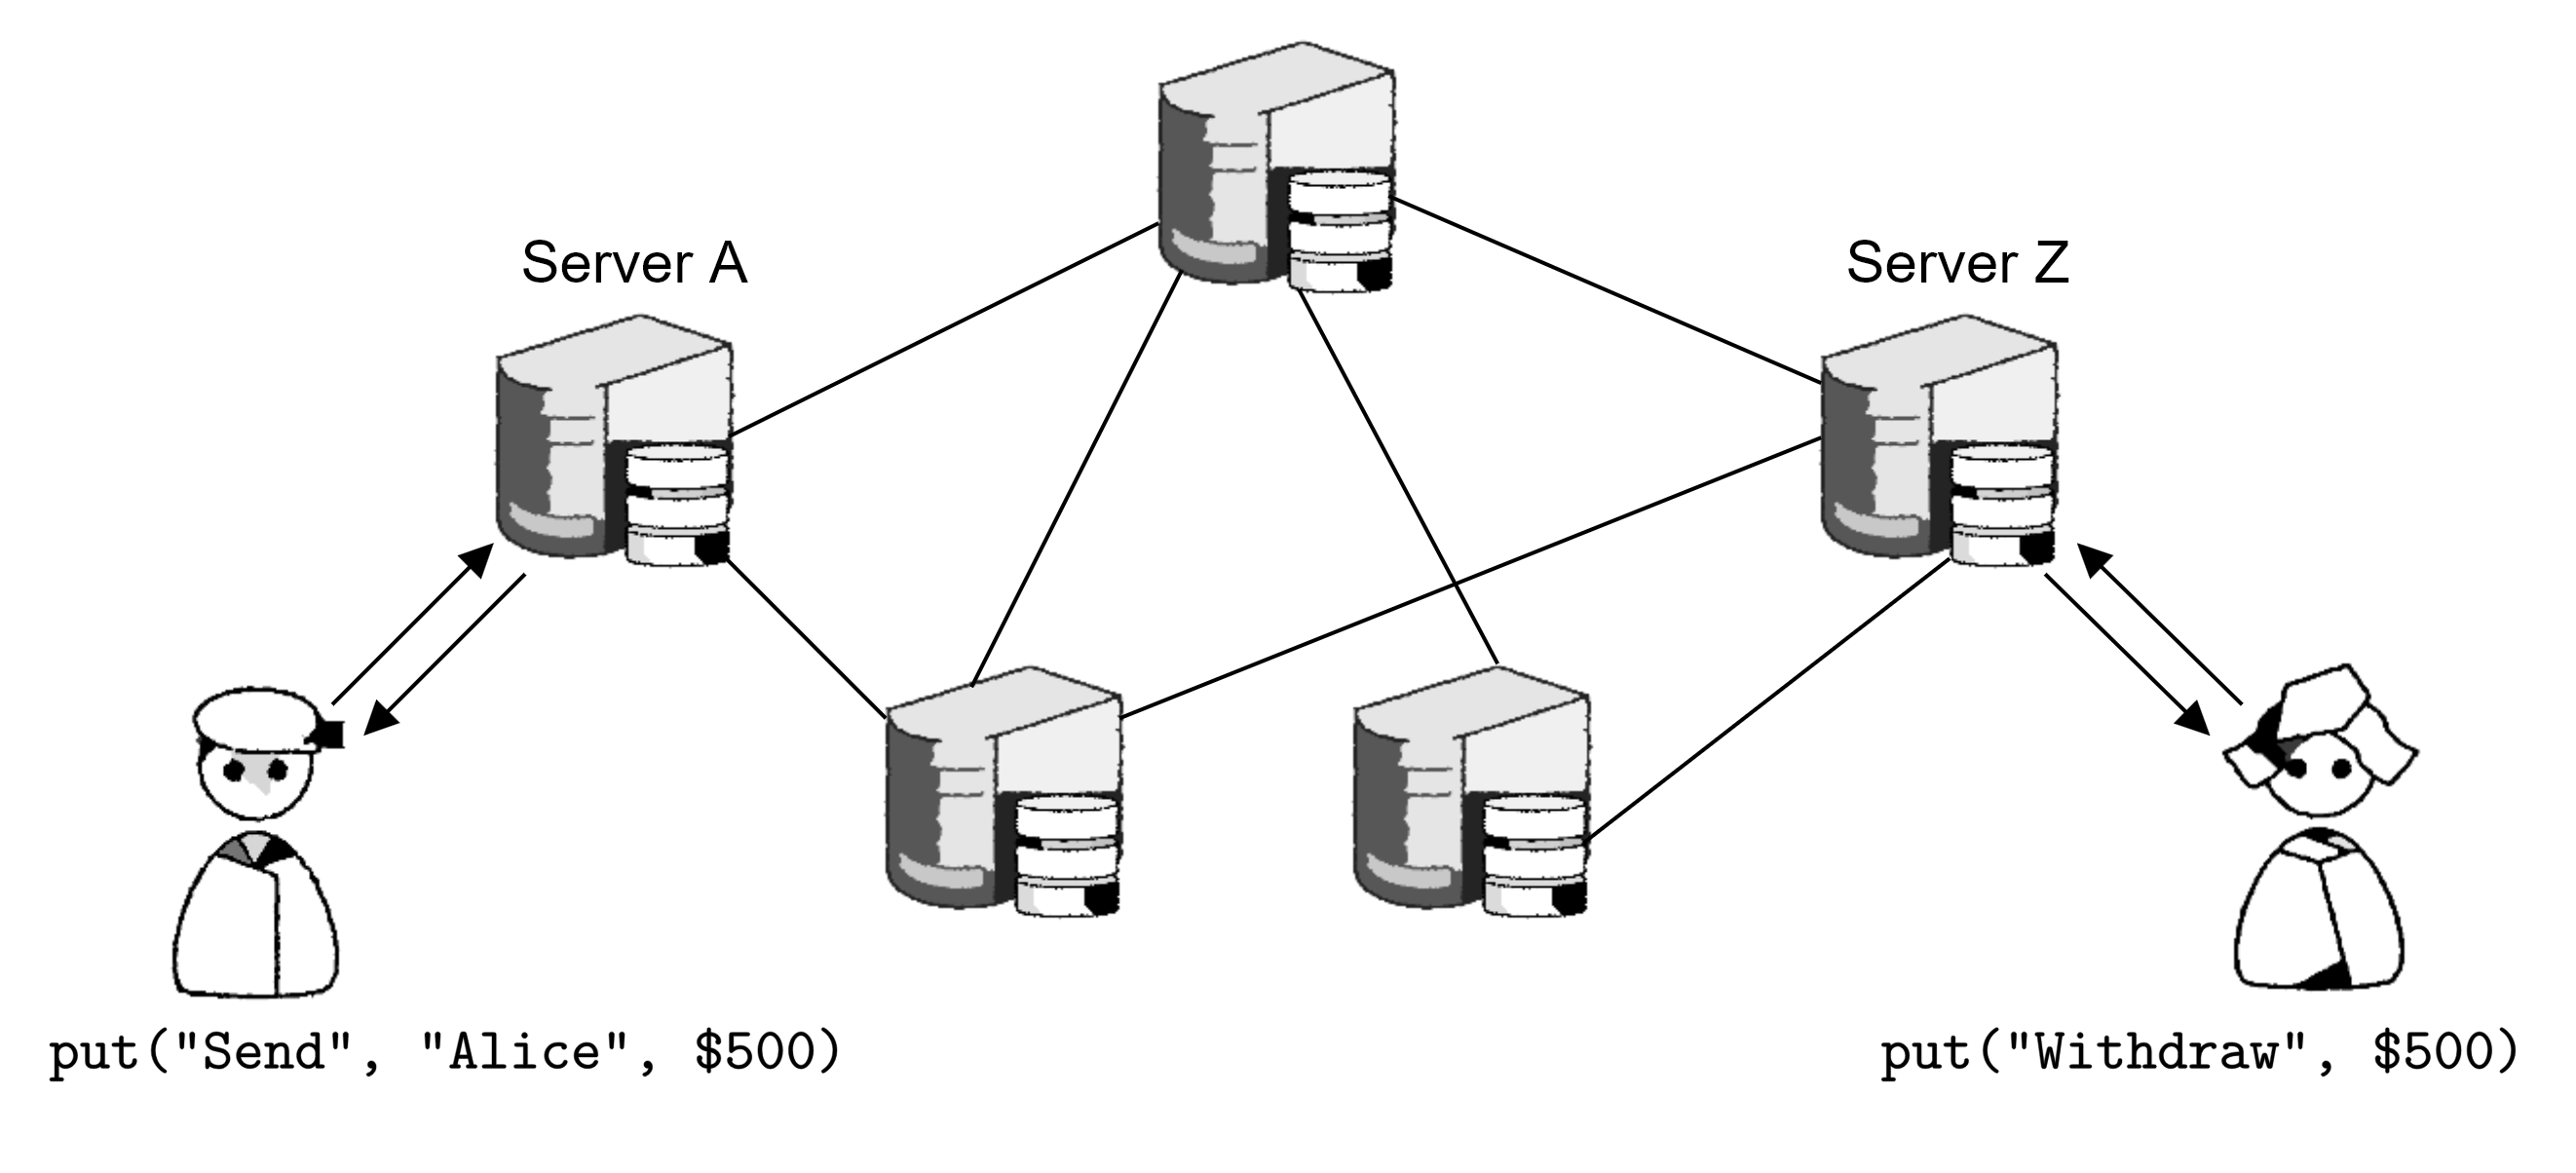
\includegraphics[width=.9\textwidth]{Sections/rep/intro.png}
    \caption{Bob sending money to Alice, while she withdraws money on two different servers.}
\end{figure}

\noindent
In this scenario Many problems can arise: What if,
\begin{itemize}
    \item The respective servers crash while or after Alice or Bob make requests?
    \item Alice and Bob share the same account, how do we ensure consistency?
\end{itemize}

\noindent
In all, wow do we ensure the propagation and synchronization of state across multiple servers?
We consider two models:
\begin{Def}[Active vs. Passive Replication]

    \textbf{Active Replication}: Client sends requests to all servers at the same time and waits for acknowledgments. This method must ensure that all 
    requests are processed in the same order (expensive).\\
    
    \noindent
    \textbf{Passive Replication}: Client sends requests to a primary server, which then forwards the request to backup servers.
\end{Def}

\newpage 

\noindent
We'll be move forward with \textbf{Passive Replication} as the preferred choice in this section.
Though it is less expensive than active replication, it still has its challenges:
\begin{itemize}
    \item \textbf{Consistency}: How do we ensure all backups are consistent?
    \item \textbf{Failure Handling}: What if the primary server fails?
    \item \textbf{Performance}: How do we ensure that the system is performant as we scale backups?
\end{itemize}

\noindent
We consider two methods of replication:
\begin{Def}[State vs. Request Replication]

    \textbf{State Replication}: Forward the entire state to backups. This results in large message sizes, but is relatively simple depending on the system.\\

    \noindent 
    \textbf{Request Replication}: Forward only requests to backups. This results in smaller message sizes, but adds complexity when requests are not deterministic (e.g., random number generation).
\end{Def}

\noindent
Still again, we run into the following problem:
\begin{figure}[h]
    \centering
    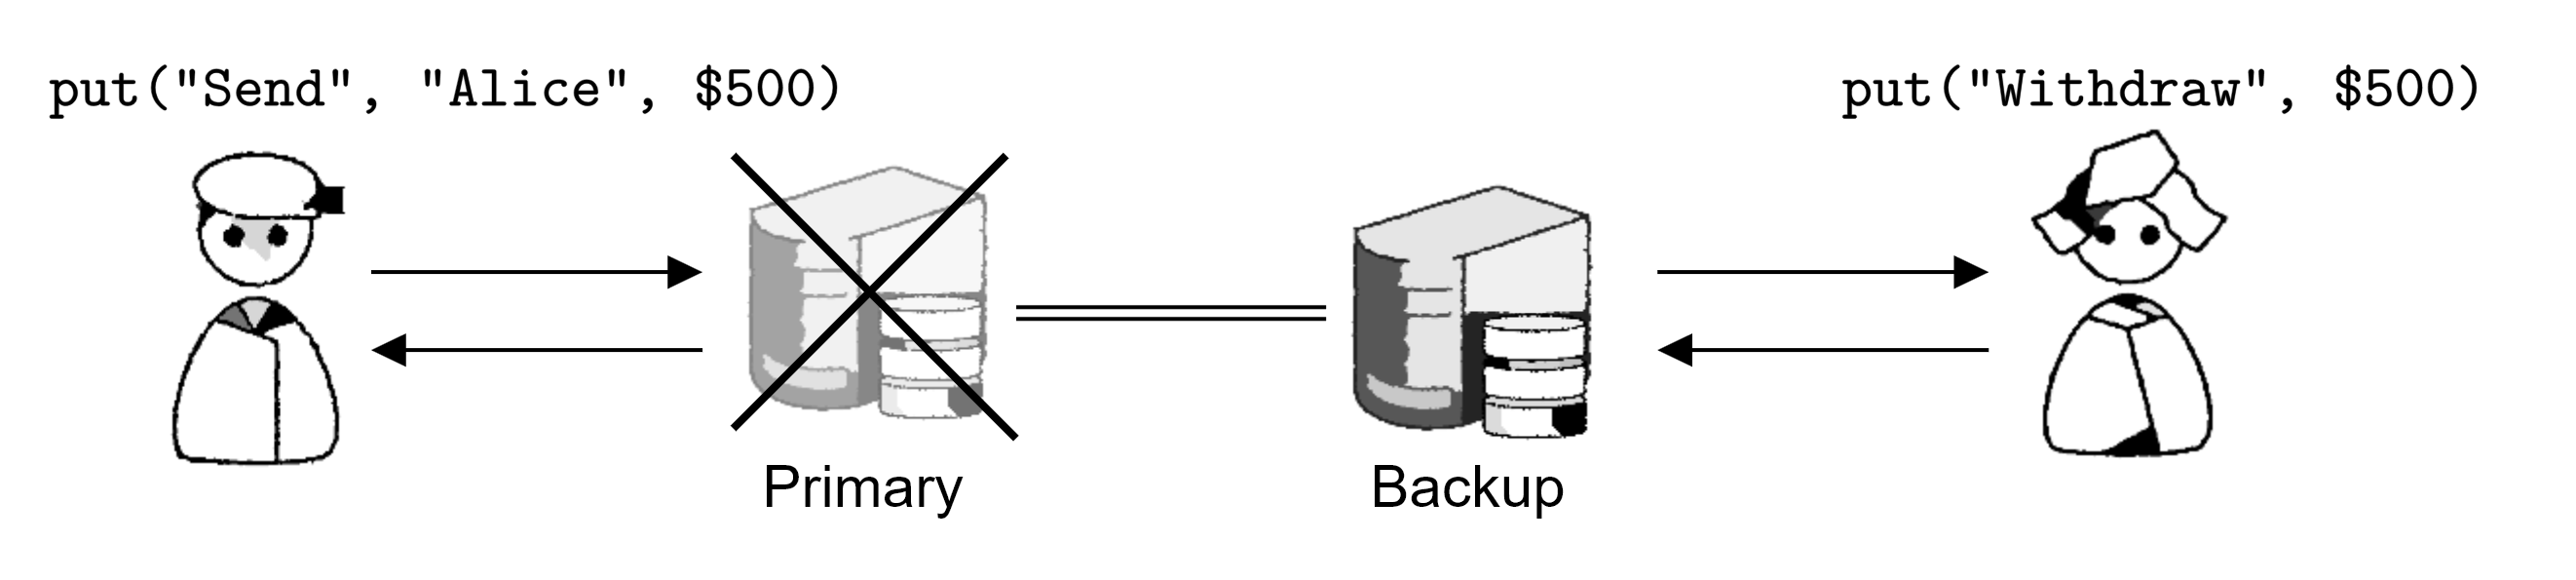
\includegraphics[width=.9\textwidth]{Sections/rep/primary.png}
    \caption{Bob's primary server failing, as Alice accesses the backup server.}
\end{figure}

\noindent
How do we ensure both parties receive consistent feedback, even when the primary server fails?
\begin{Def}[Commit Point]

    The point at which the client is committed to a transaction, goes as follows:
    \begin{enumerate}
        \item The client sends a request to the primary server and waits for an acknowledgment.
        \item The primary server forwards the request to the backup servers.
        \item The backup servers process the request and send an acknowledgment to the primary server.
        \item The primary server sends an acknowledgment to the client.
    \end{enumerate}

    \noindent
    Step 4 is considered the \textbf{commit point}.
\end{Def}

\newpage 

\noindent
The following Figure illustrates the commit point in action:
\begin{figure}[h]
    \centering
    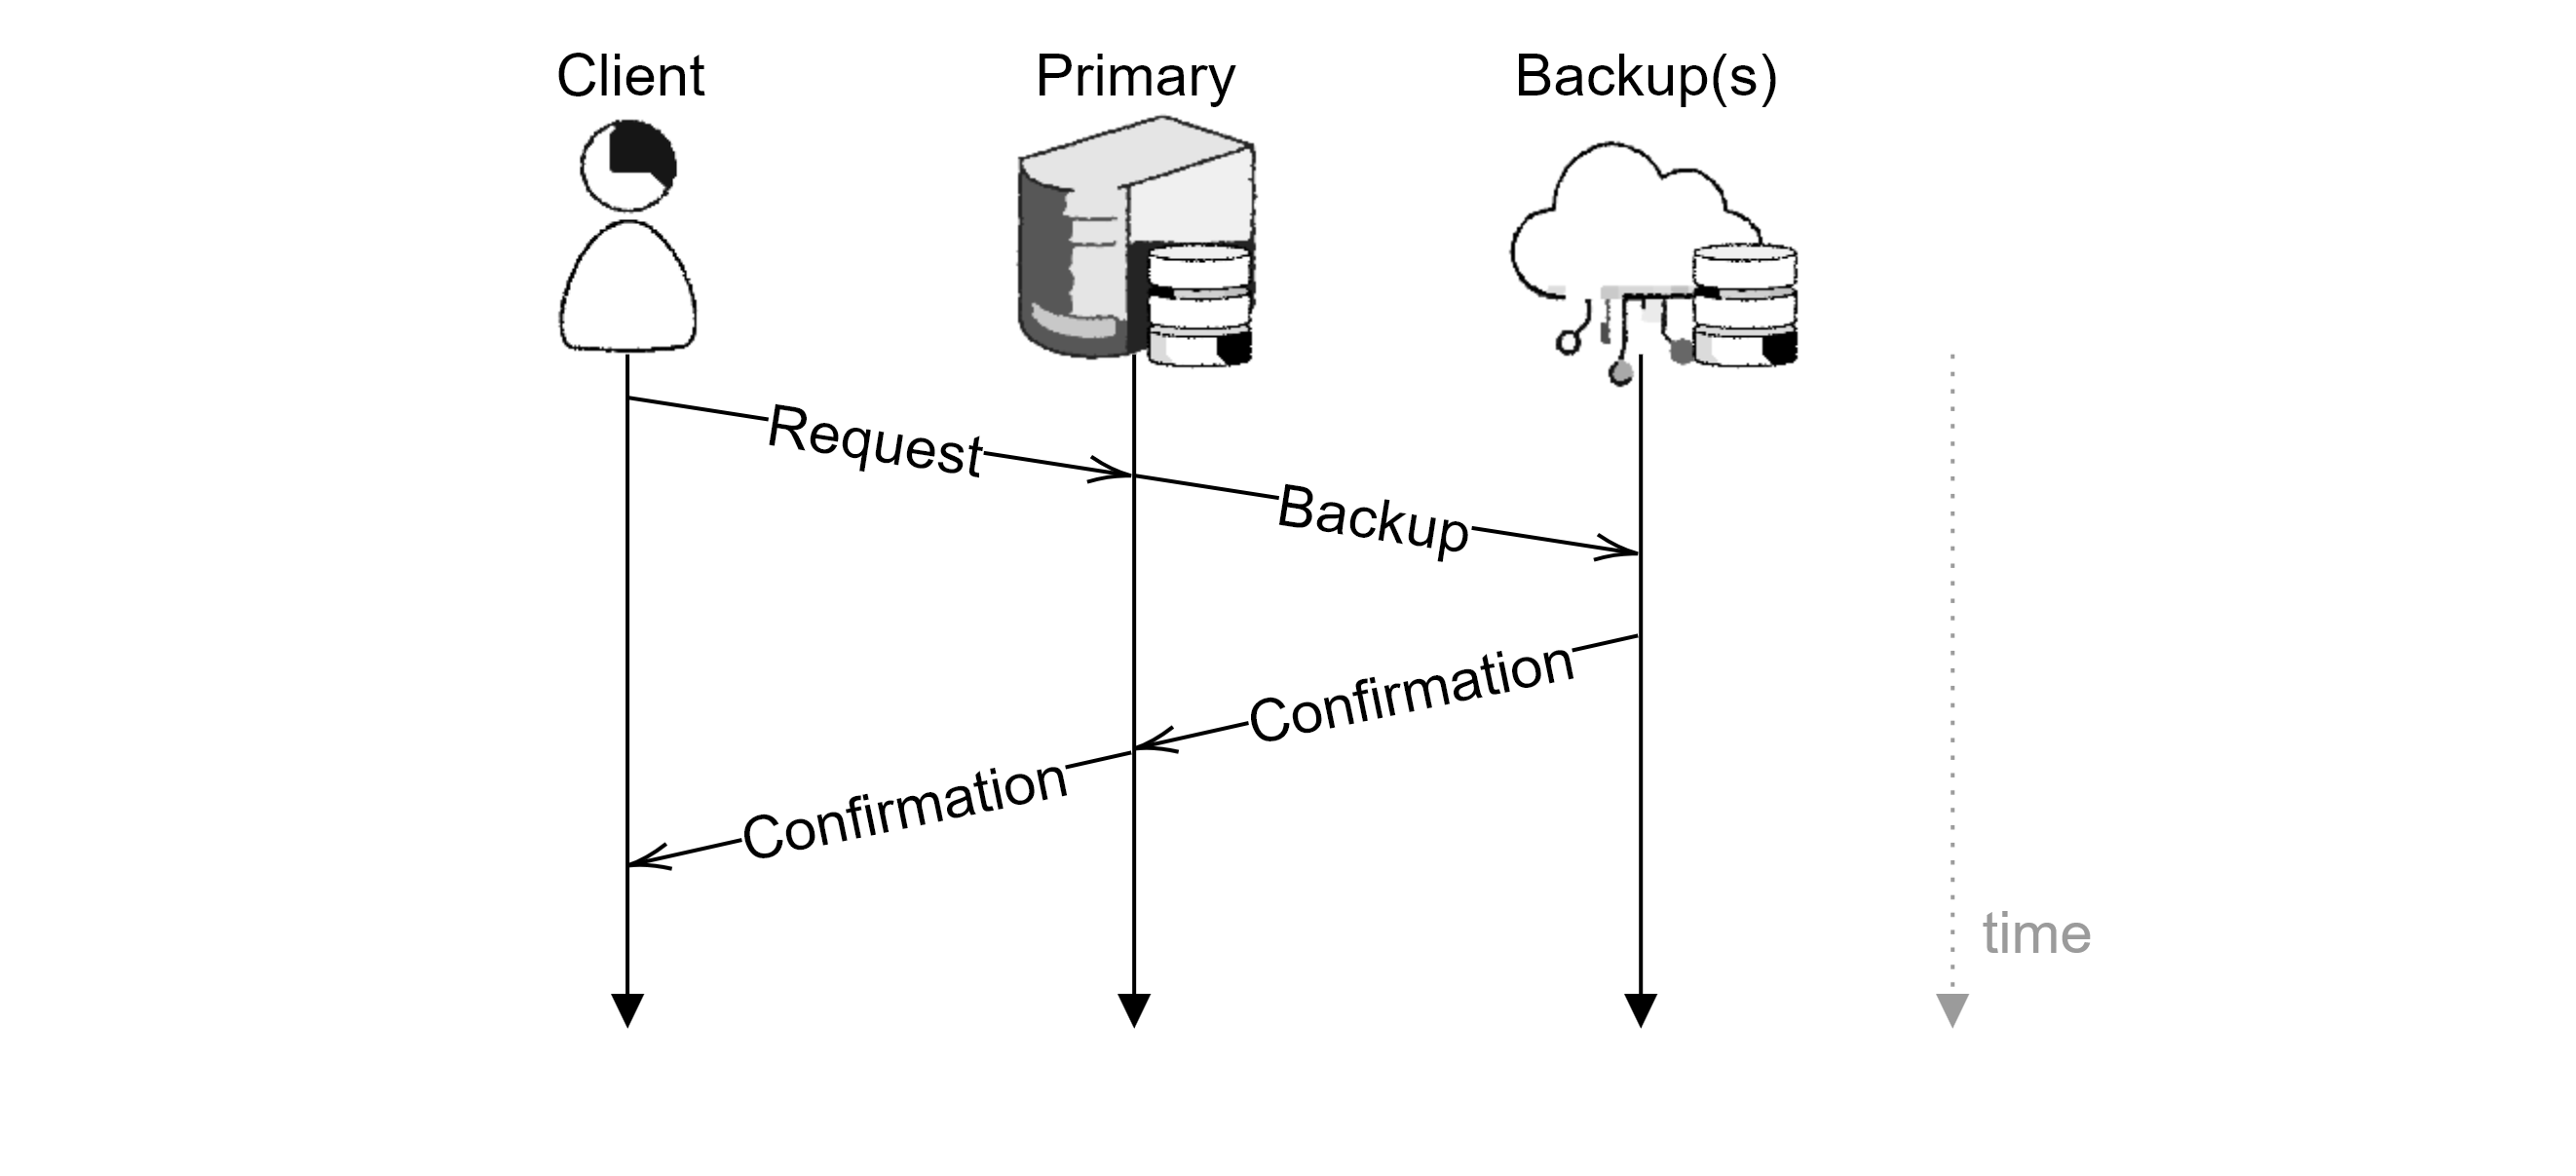
\includegraphics[width=1\textwidth]{Sections/rep/commit.png}
    \caption{Client's requests propagating through the primary and backup sever.}
\end{figure}


\input{Sections/consensus/consensus}
\section{Replication Consensus Algorithm: Raft}
As we've discussed so far, replication consistency is crucial and a 
difficult task. The next strategy, \textbf{Raft}, deals with such problem.
There are other solutions, however, Raft is considered safe and easier to 
implement correctly than other solutions. First we must familiarize ourselves with the following terms:
\begin{Def}[State Machines in Distributed Systems]
    
    A \textbf{State Machine} processes \underline{deterministic} sequence of inputs from a \textbf{log} and saves them
    in state.
    \textbf{Replicated state machines} are implemented via \textbf{replicated logs} across multiple servers
    utilizing a \textbf{Consensus Algorithm}, which validates log order.
\end{Def}

\vspace{-1em}
\begin{figure}[h]
    \centering
    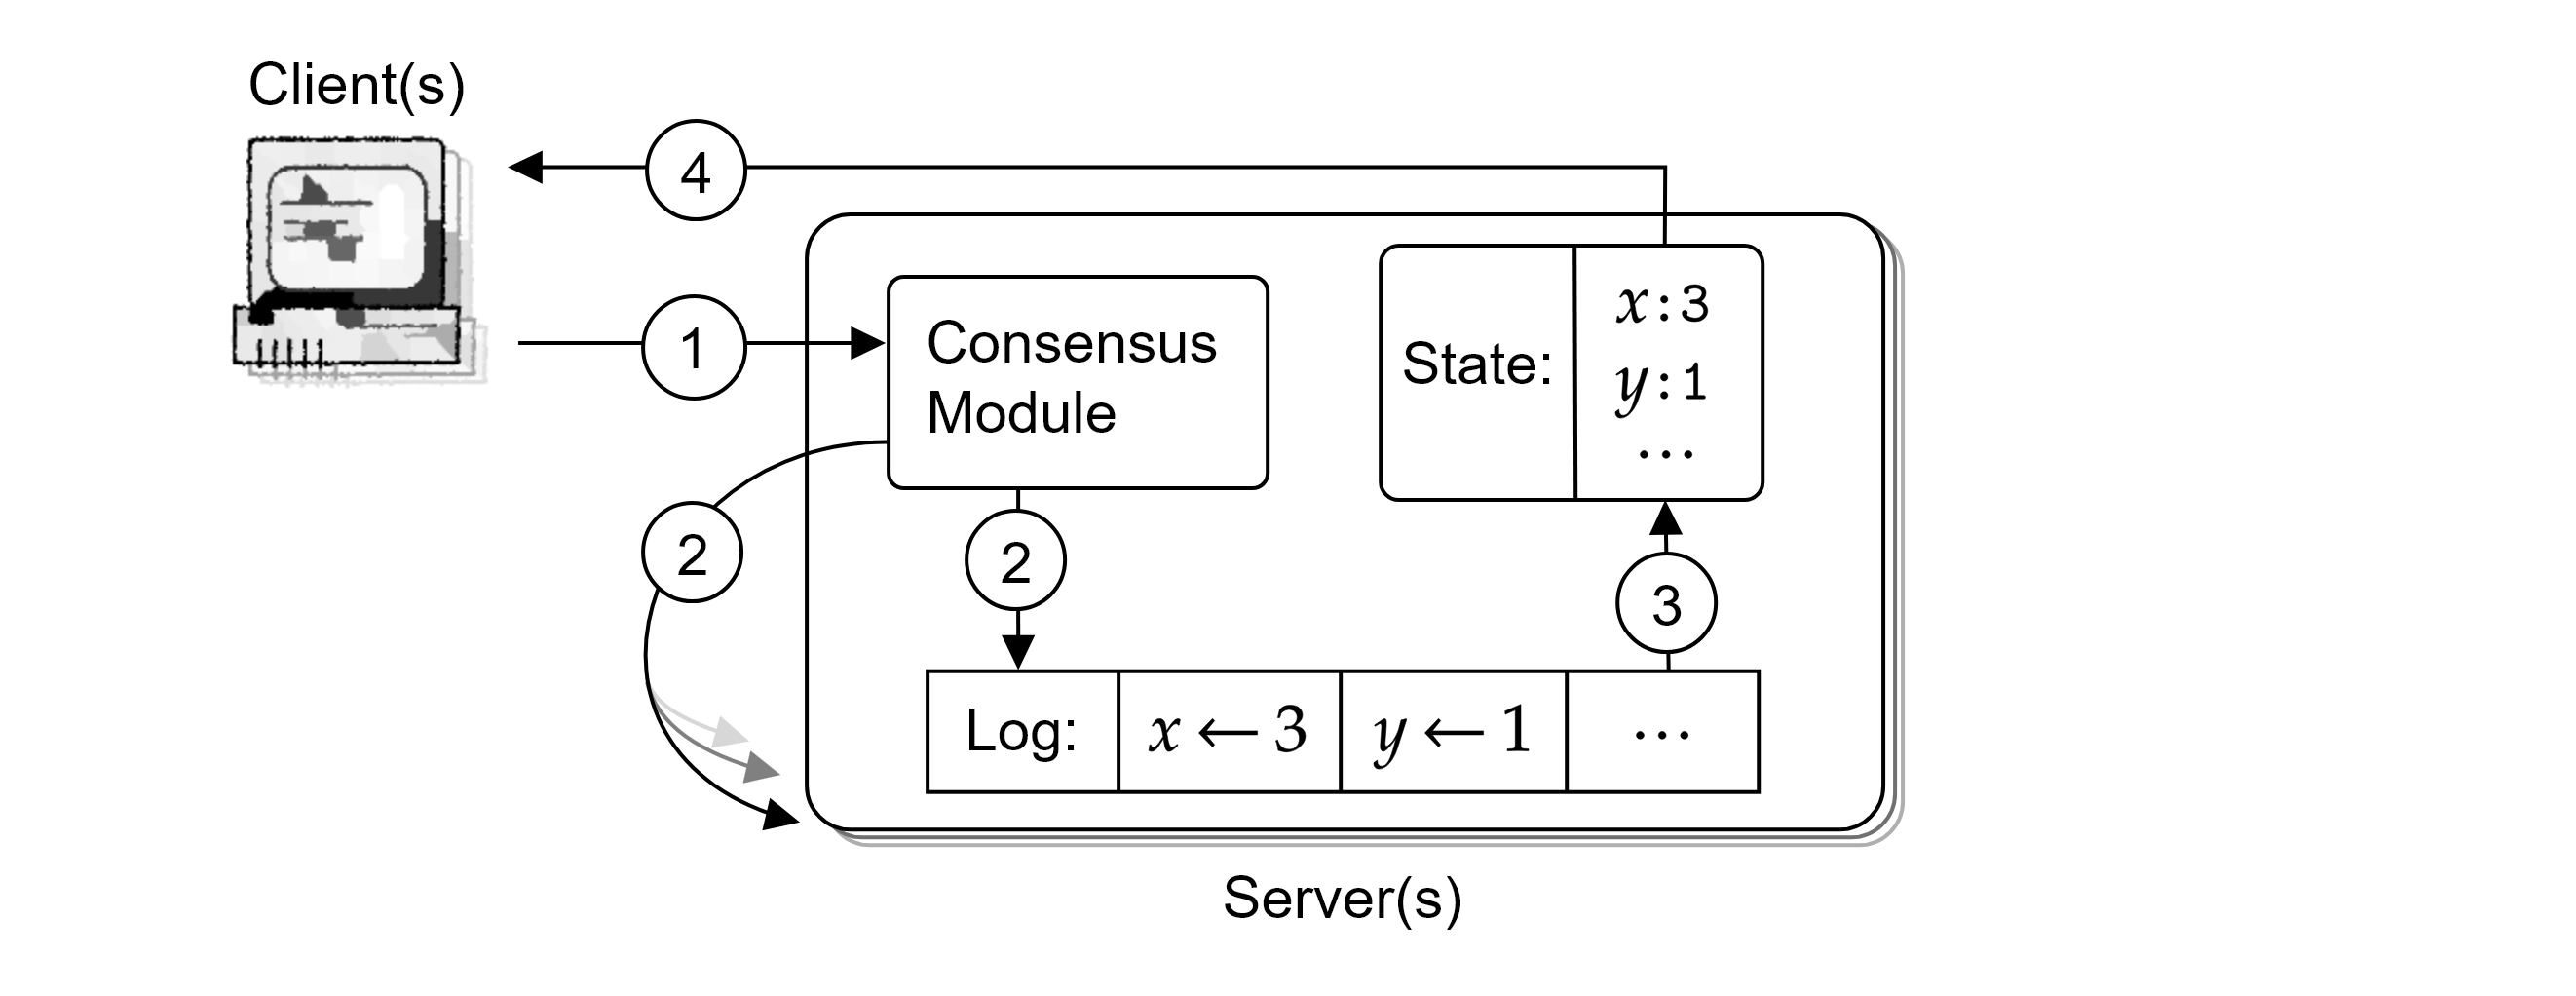
\includegraphics[width=1\textwidth]{Sections/raft/state.png}
    \caption{High-level framework for replicated state machines.}
\end{figure}
\noindent
In the above the \textbf{Consensus Module} communicates with other servers to serve consistent logs. 

\newpage 

\noindent
Now to define the parts which make up a consensus algorithm:
\begin{Def}[Consensus Algorithm Components]

    A \textbf{Consensus Algorithm} involves the following components:
    \begin{itemize}
        \item \textbf{Safety}: Always returns correct results in spite, network delays, partitions, duplications, and reorderings.
        \item \textbf{Liveness}: A \textbf{Cluster} (group of servers) must tolerate a subset of server failures (e.g., A cluster of 5 servers can tolerate 2 failures). Offline 
        servers may later recover and rejoin the cluster.
        \item \textbf{Time Agnostic}: The algorithm must not rely on synchronized clocks.
        \item \textbf{Majority Rule}: A majority of servers must agree on a value before it is committed. Minority slow servers must not block the system.
    \end{itemize}
\end{Def}

\noindent
At a high level, The Raft Algorithm:
\begin{Def}[Raft Abstract]

    The Raft Algorithm involves three main components:
    \begin{itemize}
        \item \textbf{Leader Election}: A leader $\ell$ is elected to manage the replication process of backups $\beta$.
        \item \textbf{Heartbeats}: Where $\ell$ and $\beta$ exchange consistent pulses of data to ensure liveliness.
        \item \textbf{Assurance}: Commit points (\ref{def:commit}) are established between the client, $\ell$, and $\beta$. 
    \end{itemize}
\end{Def}
\noindent
In Raft, servers are given roles to manage the replication process.
\begin{Def}[Raft Server States]

    A Raft server can be in one of the following states:
    \begin{itemize}
        \item \textbf{Follower}: A server that listens to the leader.
        \item \textbf{Candidate}: A server that is running for leader.
        \item \textbf{Leader}: A server that is managing the replication process.
    \end{itemize}
    \textbf{Followers are passive} and simply listen to the leader. \textbf{Clients interact with the leader}. Followers that are contacted \textbf{will redirect} the request to the leader.
\end{Def}

% \newpage 
\section{Failure Models}
\subsection{Defining Failures}
This section discusses, what to do or how to classify when failures occur.

\begin{Def}[Failure Model]

    A \textbf{Failure Model} is a set of assumptions about the types of failures that can occur in a distributed system.
    Such failures may be \textbf{Correlated} or \textbf{Independent}. Processes that do not fail are considered \textbf{Correct}.
\end{Def}

\noindent
In particular, we are concerned with the following types of failures:
\begin{itemize}
    \item Crash and or omission of responses, and how we might recover from them.
    \item Deviation protocol, arbitrarily or maliciously.
\end{itemize}
\begin{Def}[Crash-Stop Failure]
    
    \label{def:crash-stop}
    A \textbf{Crash-Stop Failure} occurs when a process halts and does not resume (e.g., power failure, software crash). The failure is not explicitly detectable by other processes.
    \textbf{Permanent hardware failures} typically fall under category of crash-stop failures.\\
\end{Def}

\noindent

\begin{Def}[Fail-Stop Failure]
    
    A \textbf{Fail-Stop Failure} is a detectable crash-stop failure (e.g., timeouts, heartbeats).
\end{Def}


\begin{Def}[Omission Failure]

    An \textbf{Omission Failure} can be categorized into two types:

    \begin{itemize}
        \item \textbf{Send Omission}: The process fails to send messages according to the protocol.
        \item \textbf{Receive Omission}: The process fails to receive messages that were sent by other processes.
    \end{itemize}

    \noindent
    \textbf{In particular}, The process itself may still be operational but unable to correctly communicate (e.g., network disruptions, software errors, or buffer overflows).
\end{Def}

\newpage 

\begin{Def}[Crash-Recovery Failure]

    A \textbf{Crash-Recovery Failure} occurs when a process halts due to a crash but retains the \textbf{ability to recover} and resume execution. 

    \begin{itemize}
        \item \textbf{Crash Phase}: The process halts in some way (e.g., stops sending or receiving messages).
        \item \textbf{Recovery Phase}: The processes may recover to the last correct state via snapshot (\ref{sec:snap}). Certain types of memory may persist through the crash:
        \begin{itemize}
            \item \textbf{Volatile memory} is lost during a crash (e.g, mid-execution variables).
            \item \textbf{Stable storage} is retained through a crash (e.g., disk storage, assuming no disk failure).
        \end{itemize}
    \end{itemize}

    \noindent
    \textbf{However,} if the processes crashes indefinitely, it is considered a \textbf{Crash-Stop} failure (\ref{def:crash-stop}).
\end{Def}

\begin{Def}[Byzantine Failure]

    A \textbf{Byzantine Failure} occurs when a process exhibits arbitrary or malicious behavior, leading to unpredictable system behavior.

    \begin{itemize}
        \item \textbf{Arbitrary Behavior}: The process deviates from the expected protocol, such as:
        \begin{itemize}
            \item Sending corrupted or inconsistent messages to different nodes.
            \item Updating its state in an unintended or unpredictable manner.
        \end{itemize}

        \item \textbf{Malicious Behavior}: The process actively attempts to disrupt the system, such as:
        \begin{itemize}
            \item Exploiting protocol vulnerabilities to manipulate outcomes (e.g., double-spending in a blockchain).
        \end{itemize}
    \end{itemize}

    \noindent
    In short, these failures occur due to \textbf{bugs} (unintentional) or \textbf{attacks} (intentional).
\end{Def}

\begin{Tip} The term \textbf{Byzantine} in computer science comes from the \textit{Byzantine Generals Problem}, introduced by Leslie Lamport in 1982. It describes a scenario where generals must coordinate an attack but cannot trust all messengers—some may be traitors sending conflicting information.

    The name \textit{Byzantine} is inspired by the Byzantine Empire, which was historically known for its complex and often deceptive political intrigues. While the term is widely used in distributed systems, some argue it unfairly portrays Byzantine history.

    In computing, a \textbf{Byzantine failure} refers to a system component acting unpredictably, whether due to bugs, faults, or malicious intent, making consensus difficult.

\end{Tip}

\newpage

\subsection{Failures Model Hierarchy}

As we compare failure models as extensions of each other. Here we will omit \textbf{fail-stop} as it is more of a detection mechanism.
To quickly recap:
\begin{itemize}
    \item \textbf{Crash-Stop}: Process halts and cannot resume (undetectable).
    \item \textbf{Omission}: Process fails to properly communicate.
    \item \textbf{Crash-Recovery}: Process halts but can recover and resume.
    \item \textbf{Byzantine}: Process exhibits arbitrary or malicious behavior.
\end{itemize}

\begin{theo}[Failure Model Hierarchy]

    The failure models can be arranged in a hierarchy, where each model is an extension of the previous one. 
    The hierarchy is as follows:
    \begin{center}
        \textbf{Crash-Stop} $\subset$ \textbf{Omission} $\subset$ \textbf{Crash-Recovery} $\subset$ \textbf{Byzantine}
    \end{center}
    In particular, 
    \begin{itemize}
        \item \textbf{Crash-Stop} $\subset$ \textbf{Omission}, as a crash-stop failure is stricter, meaning a full crash, rather than a partial communication failure.
        \item \textbf{Omission} $\subset$ \textbf{Crash-Recovery}, as during recovery the last correct state, volatile memory lost may exhibit omission-like behavior. Meaning some messages are lost, due to ``\textbf{amnesia}.''
        \item \textbf{Crash-Recovery} $\subset$ \textbf{Byzantine}, as a process may recover and exhibit arbitrary or malicious behavior. Moreover, a Byzantine failure may mean \textbf{any type of failure}.
    \end{itemize}
\end{theo}

\begin{figure}[h]
    \centering
    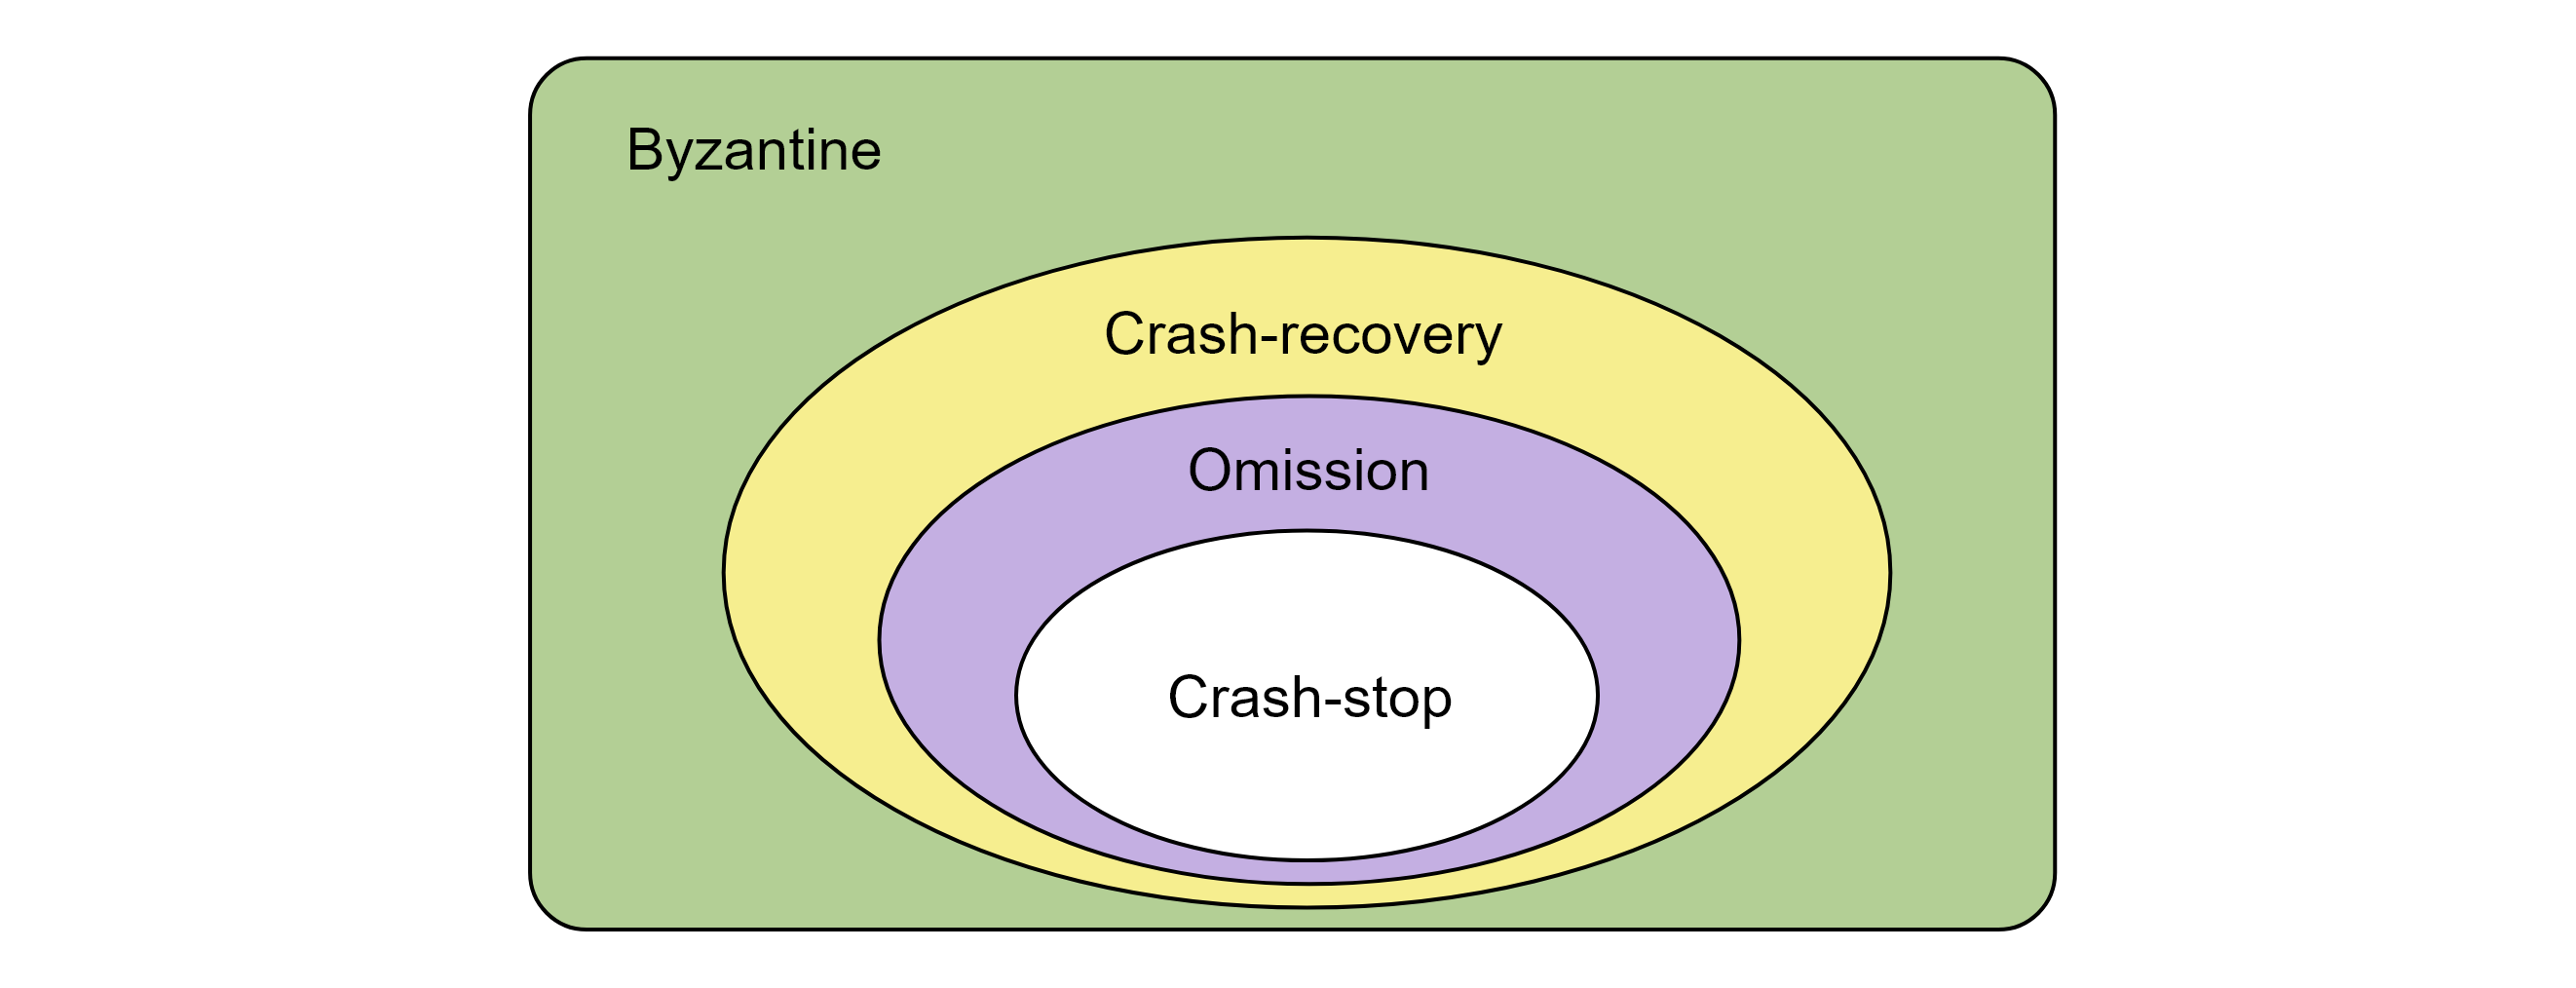
\includegraphics[width=\textwidth]{Sections/crash/fail.png}
    \caption{Failure Hierarchy depicting: Crash-stop $\subset$ Omission $\subset$ Crash-Recovery $\subset$ Byzantine}
\end{figure}





\bibliographystyle{plain} % We choose the "plain" reference style
\bibliography{refs} % Entries are in the refs.bib file



\end{document}
